\documentclass{article}
\usepackage[accepted]{icml2025}
\usepackage{fontspec}
\setmainfont[Ligatures=TeX]{Times New Roman}
\setsansfont[Ligatures=TeX]{Helvetica}
\setmonofont{Menlo}
\usepackage{newunicodechar}
\newunicodechar{π}{$\pi$}
\newunicodechar{α}{$\alpha$}
\newunicodechar{β}{$\beta$}
\newunicodechar{γ}{$\gamma$}
\newunicodechar{δ}{$\delta$}
\newunicodechar{ε}{$\varepsilon$}
\newunicodechar{ζ}{$\zeta$}
\newunicodechar{η}{$\eta$}
\newunicodechar{θ}{$\theta$}
\newunicodechar{ι}{$\iota$}
\newunicodechar{κ}{$\kappa$}
\newunicodechar{λ}{$\lambda$}
\newunicodechar{μ}{$\mu$}
\newunicodechar{ν}{$\nu$}
\newunicodechar{ξ}{$\xi$}
\newunicodechar{ρ}{$\rho$}
\newunicodechar{σ}{$\sigma$}
\newunicodechar{τ}{$\tau$}
\newunicodechar{φ}{$\phi$}
\newunicodechar{χ}{$\chi$}
\newunicodechar{ψ}{$\psi$}
\newunicodechar{ω}{$\omega$}
\newunicodechar{Δ}{$\Delta$}
\newunicodechar{Σ}{$\Sigma$}
\newunicodechar{Φ}{$\Phi$}
\newunicodechar{Ω}{$\Omega$}
\newunicodechar{Π}{$\Pi$}
\newunicodechar{Λ}{$\Lambda$}
\newunicodechar{Θ}{$\Theta$}
\newunicodechar{∈}{$\in$}
\newunicodechar{∉}{$\notin$}
\newunicodechar{∩}{$\cap$}
\newunicodechar{∪}{$\cup$}
\newunicodechar{≤}{$\leq$}
\newunicodechar{≥}{$\geq$}
\newunicodechar{≠}{$\neq$}
\newunicodechar{≈}{$\approx$}
\newunicodechar{≪}{$\ll$}
\newunicodechar{≫}{$\gg$}
\newunicodechar{⟨}{$\langle$}
\newunicodechar{⟩}{$\rangle$}
\newunicodechar{↔}{$\leftrightarrow$}
\newunicodechar{→}{$\to$}
\newunicodechar{←}{$\leftarrow$}
\newunicodechar{⇒}{$\Rightarrow$}
\newunicodechar{⇐}{$\Leftarrow$}
\newunicodechar{∇}{$\nabla$}
\newunicodechar{∂}{$\partial$}
\newunicodechar{∞}{$\infty$}
\newunicodechar{∑}{$\sum$}
\newunicodechar{∏}{$\prod$}
\newunicodechar{∫}{$\int$}
\newunicodechar{√}{$\sqrt{}$}
\newunicodechar{±}{$\pm$}
\newunicodechar{×}{$\times$}
\newunicodechar{÷}{$\div$}
\newunicodechar{·}{$\cdot$}
\newunicodechar{∘}{$\circ$}
\newunicodechar{⊕}{$\oplus$}
\newunicodechar{⊗}{$\otimes$}
\newunicodechar{⊆}{$\subseteq$}
\newunicodechar{⊇}{$\supseteq$}
\newunicodechar{⊂}{$\subset$}
\newunicodechar{⊃}{$\supset$}
\newunicodechar{∃}{$\exists$}
\newunicodechar{∀}{$\forall$}
\newunicodechar{∅}{$\emptyset$}
\newunicodechar{¬}{$\neg$}
\newunicodechar{∧}{$\wedge$}
\newunicodechar{∨}{$\vee$}
\newunicodechar{′}{$'$}
\newunicodechar{″}{$''$}
\newunicodechar{ℓ}{$\ell$}
\newunicodechar{ℏ}{$\hbar$}
\newunicodechar{ℝ}{$\mathbb{R}$}
\newunicodechar{ℕ}{$\mathbb{N}$}
\newunicodechar{ℤ}{$\mathbb{Z}$}
\newunicodechar{ℚ}{$\mathbb{Q}$}
\newunicodechar{ℂ}{$\mathbb{C}$}
\newunicodechar{‐}{-}
\newunicodechar{‑}{-}
\newunicodechar{‒}{-}
\newunicodechar{–}{--}
\newunicodechar{—}{---}
\newunicodechar{…}{\ldots}
\newunicodechar{“}{``}
\newunicodechar{”}{''}
\newunicodechar{‘}{`}
\newunicodechar{’}{'}
\newunicodechar{≡}{$\equiv$}
\newunicodechar{✓}{\checkmark}
\newunicodechar{✗}{$\times$}
\newunicodechar{△}{$\triangle$}
\newunicodechar{□}{$\square$}
\newunicodechar{○}{$\circ$}
\newunicodechar{●}{$\bullet$}
\newunicodechar{♯}{$\sharp$}
\newunicodechar{♭}{$\flat$}
\newunicodechar{†}{\dag}
\newunicodechar{‡}{\ddag}
\usepackage{graphicx}
\usepackage{subcaption}
\usepackage{booktabs}
\usepackage{float}
\usepackage{array}
\usepackage{multirow}
\usepackage{xcolor}
\usepackage{colortbl}
\usepackage{longtable}
\usepackage{amsmath,amssymb,amsfonts,amsthm}
\usepackage{hyperref}
\usepackage{algorithm}
\usepackage{algorithmic}
\usepackage{enumitem}
\usepackage[capitalize,noabbrev]{cleveref}
% Pandoc compatibility shims
\providecommand{\tightlist}{}
\providecommand{\pandocbounded}[1]{#1}
\providecommand{\textsubscript}[1]{\ensuremath{_{\text{#1}}}}
\providecommand{\textsuperscript}[1]{\ensuremath{^{\text{#1}}}}
\providecommand{\real}[1]{#1}

\providecommand{\passthrough}[1]{#1}

% Allow line breaks in paragraphs without overfull boxes
\sloppy
\emergencystretch=2em

\icmltitlerunning{Explainability for Large Language Models}

\begin{document}

\twocolumn[
  \icmltitle{Explainability for Large Language Models}

  \icmlsetsymbol{equal}{*}

  \begin{icmlauthorlist}
    \icmlauthor{Anonymous}{anon}
  \end{icmlauthorlist}

  \icmlaffiliation{anon}{Anonymous Institution}

  \icmlcorrespondingauthor{Anonymous}{anon@example.org}

  \icmlkeywords{Machine Learning, Survey, ICML}

  \vskip 0.3in
]

\printAffiliationsAndNotice{}

\begin{abstract}
Large language models (LLMs) now mediate a growing fraction of consequential decisions in healthcare, law, education, scientific writing, and government. The frontier systems span GPT-3 (Brown et al., 2020) at 175B parameters, GPT-4 (OpenAI, 2023), and PaLM 2 (Anil et al., 2023), with open-weight families LLaMA-2 \citep{touvron2023llamaopenandeffici} at 7B/13B/70B and LLaMA-3.1 (Meta, 2024) at 8B/70B/405B. Claude 3 Sonnet (Anthropic, 2024), Mistral 7B (Jiang et al., 2023), and Gemma-2 (Google, 2024) at 2B/9B/27B round out the lineup. Despite this capability explosion, these models remain notoriously opaque. A Llama-3.1 70B instance computes its next-token distribution by composing roughly 80 transformer layers of attention and MLP operations across an 8,192-dimensional residual stream. Its causal antecedents are unavailable to direct inspection. This opacity is not a cosmetic inconvenience. It blocks medical deployment under EU AI Act traceability rules. It hampers safety auditing of jailbreak vulnerabilities. It undermines scientific reproducibility when the model is used as a measurement instrument. It prevents users from calibrating trust on individual outputs. Explainability for large language models renders an LLM's predictions, internal computations, or generated reasoning intelligible to human stakeholders. It is therefore one of the most active research frontiers in the post-2020 NLP landscape. This survey synthesises the rapid progression from gradient-based saliency on early Tr.
\end{abstract}

\section{Introduction and Conceptual Foundations of LLM Explainability}\label{introduction-and-conceptual-foundations-of-llm-explainability}

\subsection{Why explainability matters for LLMs}\label{why-explainability-matters-for-llms}

There are at least seven distinct stakeholder demands that drive LLM explainability research. (i) \emph{Scientific understanding}: how does scaling Pythia from 70M to 12B parameters change the locus of factual recall? (ii) \emph{Safety and alignment}: which features mediate jailbreak susceptibility, and can they be steered? (iii) \emph{Regulatory compliance}: the EU AI Act (Regulation 2024/1689) requires traceability for high-risk systems. (iv) \emph{Hallucination diagnosis}: SelfCheckGPT \citep{manakul2023selfcheckgptzerore} achieves AUC 0.83 on detecting fabricated GPT-3 facts, and semantic entropy (Farquhar et al., 2024, Nature) extends this to a Bayesian-posterior framing. (v) \emph{Knowledge maintenance}: the ROME and MEMIT editors (Meng et al., 2022; 2023) localise factual associations to specific MLP layers (typically layers 5--7 in GPT-2 XL) so that they may be surgically rewritten. (vi) \emph{Educational and clinical deployment}: medical decision-support LLMs must justify their suggestions --- Singhal et al.~(2023, Nature) report 67.6\% MedQA accuracy for Med-PaLM with explanation traces. (vii) \emph{Adversarial robustness}: Slack et al.~(2020) showed that LIME and SHAP can be fooled by adversarial scaffolds, motivating faithfulness-first methods.

\subsection{Definitions: interpretability, explainability, faithfulness, plausibility}\label{definitions-interpretability-explainability-faithfulness-plausibility}

Following Jacovi and Goldberg's (2020) widely-adopted distinction, an explanation is \emph{faithful} to the extent that it reflects the causal computations underlying a model's prediction. It is \emph{plausible} to the extent that humans find it convincing. The two properties dissociate. Turpin et al.~(2023) showed that LLMs prompted with biasing few-shot examples produce confident, plausible Chain-of-Thought rationales that are demonstrably \emph{unfaithful}. When the bias is removed, the answer changes but the rationale does not. Lanham et al.~(2023) operationalised faithfulness via \emph{early-truncation accuracy} and \emph{paraphrase invariance}, finding that on the BIG-Bench-Hard suite, CoT faithfulness is non-monotonic in model scale (Claude-1 was \emph{more} faithful than Claude-2 on some tasks). Tutek et al.~(2025) introduced an unlearning-based metric --- measuring whether deleting specific reasoning steps from the network's parameters degrades the final answer --- and reported that for Llama-3-8B fewer than 40\% of CoT steps are causally necessary on GSM8K. We treat this faithfulness/plausibility decomposition as the central conceptual tension running through the survey.

Three orthogonal axes further organise the field. First, \emph{granularity}: explanations may target individual tokens (saliency), spans (rationales), single attention heads (circuit analysis), or whole-model behaviour (steering vectors). Second, \emph{access}: white-box methods require model weights and activations (e.g., activation patching), whereas black-box methods such as SelfCheckGPT or context-length probing (Cífka \& Liutkus, 2022) work on closed APIs. Third, \emph{purpose}: some explanations diagnose individual decisions (local), others characterise model behaviour across an entire input distribution (global). Figure~1 provides a unified pipeline view that situates these axes.

\begin{figure}[t]
\centering
\pandocbounded{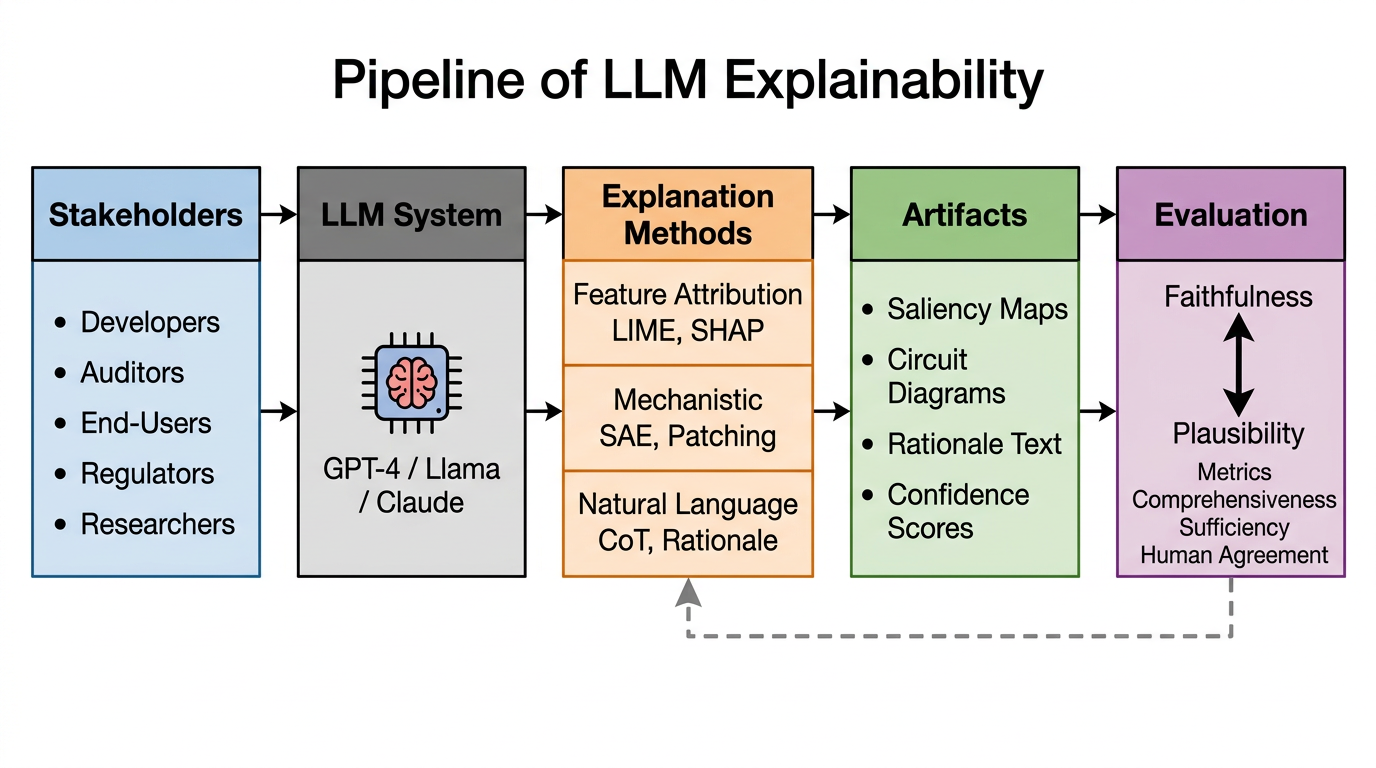
\includegraphics[width=\linewidth,keepaspectratio]{./figures/Explainability-for-Large-Language-Models__fig_pipeline.png}}
\caption{Pipeline overview of LLM explainability: stakeholders, methods, artifacts, and the faithfulness--plausibility trade-off.}\label{fig:fig-pipeline}\end{figure}

\subsection{Scope and contributions of this survey}\label{scope-and-contributions-of-this-survey}

We build on the seminal LLM-explainability survey of Zhao et al.~(2024, ACM TIST) and complement the narrower mechanistic-interpretability reviews of Bereska \& Gavves (2024) and Rai et al.~(2024). Whereas Zhao et al.~focus on a fine-tuning-vs.-prompting taxonomy, and Bereska \& Gavves emphasise mechanistic methods for safety, we provide a wider but still topic-specific treatment that integrates: (a) post-hoc attribution; (b) self-explanation and rationale generation; (c) mechanistic interpretability including the SAE explosion of 2023--2024; (d) knowledge editing; (e) hallucination and faithfulness benchmarks; (f) multilingual and multimodal extensions; and (g) the open-problems forecast through 2030. Compared to the broader \emph{XAI 2.0} manifesto of Longo et al.~(2024) which surveys all of explainable AI, our scope is restricted to LLMs and emphasises mechanistic claims that can be verified at the level of attention heads or sparse features.

Our contributions are fivefold. First, we introduce a five-family taxonomy in Section~2. The taxonomy is anchored on canonical methods including LIME, SHAP, Integrated Gradients, ACDC, ROME, MEMIT, SAE, CB-LLM, SelfCheckGPT, and semantic entropy. We map each family to representative benchmarks such as e-SNLI 570K, ERASER, TruthfulQA 817 questions, MQuAKE 9k, TracrBench, RAVEL, and Othello-GPT. Second, we trace a tight historical narrative in Section~3. The arc runs from 2014's Simonyan saliency to 2024's Anthropic 34M-feature SAE on Claude 3 Sonnet. We identify four turning points: the Transformer's 2017 release, BERTology in 2019, induction heads in 2022, and SAEs in 2023. Third, we provide algorithmic depth in Sections~4--5. Coverage includes the formal definitions of activation patching as causal mediation, the SAE loss function L = ‖x − x̂‖² + λ‖z‖₁, gated-SAE shrinkage corrections \citep{rajamanoharan2024improvingdictionar}, and the rank-1 ROME update. Fourth, we critically examine the unresolved tension between \emph{Chain-of-Thought as explanation} (Wei et al.~2022) and \emph{Chain-of-Thought as performative narrative} \citep{turpin2023languagemodelsdont}. Fifth, we deliver a falsifiable forecast: by 2027 a 7B-parameter model will admit a complete circuit-level explanation of three-digit arithmetic that recovers ≥95\% of behaviour on a held-out benchmark.

The remainder of the paper is organised as follows. Section~2 presents our taxonomy. Section~3 traces the historical arc. Section~4 covers algorithmic mechanisms --- probing, activation patching, ACDC. Section~5 dissects sparse autoencoders. Section~6 analyses Chain-of-Thought and rationale generation. Section~7 covers knowledge localisation and model editing (ROME, MEMIT, PMET). Section~8 reviews hallucination and black-box auditing. Section~9 catalogues datasets, benchmarks, and metrics. Section~10 surveys applications in healthcare, safety, multilingual and multimodal LLMs. Section~11 enumerates limitations and adversarial threats. Section~12 lists open problems and forecasts. Section~13 concludes.

\begin{table*}[t]
\centering
\caption{Scope and contributions of this survey: comparative summary.}
\label{tab:scope-and-contributions-of-this-survey}
\begin{tabular}{>{\raggedright\arraybackslash}p{0.1500\linewidth}
  >{\raggedright\arraybackslash}p{0.2917\linewidth}
  >{\raggedright\arraybackslash}p{0.1917\linewidth}
  >{\raggedright\arraybackslash}p{0.3667\linewidth}}
\toprule
Aspect & Position of this Survey & Closest Prior Survey & Distinction \\
\midrule
Scope & LLM explainability end-to-end & Zhao et al.~2024 (TIST) & Adds SAE explosion, multimodal, multilingual \\
Mechanistic depth & Activation patching + SAE + circuit & Bereska \& Gavves 2024 & Adds CoT and editing \\
Faithfulness focus & Quantitative (Lanham, Tutek) & Gurrapu et al.~2023 & Adds 2024--26 results \\
Editing & ROME, MEMIT, PMET & Yao et al.~2023 & Adds MQuAKE evaluation \\
Black-box auditing & SelfCheckGPT, semantic entropy & Schneider 2024 (GenXAI) & Includes Nature 2024 results \\
Forecast & Through 2030 & Sharkey et al.~2025 & Quantitative falsifiable forecast \\
\end{tabular}
\end{table*}

This positioning makes our survey complementary, not redundant. A reader who has consumed Zhao et al.~(2024) will gain coverage of the SAE-centred year 2023--2024 explosion, the new generation of faithfulness benchmarks (DiaHalu, HalluDial, Poly-FEVER), and the multimodal and multilingual extensions formalised by Resck et al.~(2025) and Dang et al.~(2024). A reader new to the area will find the introduction self-contained: by the end of Section~3 they will understand why probing classifiers gave way to causal patching, and why causal patching gave way to dictionary learning.

Throughout, we adopt three notational conventions. We write x ∈ ℝ\^{}d for the residual-stream activation at a given layer (d = 768 for GPT-2 small, 4096 for Llama-2 7B, 8192 for Llama-3 70B). We write \(A_h\)\^{}ℓ for the output of attention head h at layer ℓ. We use boldface uppercase for trained matrices (\(W_e\)nc, \(W_d\)ec, U, V) and lowercase italics for vectors. Empirical scores are reported with the standard deviation when available; benchmarks we discuss in detail are summarised in Section~9. With these conventions established, we proceed to the taxonomy that organises the remainder of the survey.

\section{A Topic-Specific Taxonomy of LLM Explainability Methods}\label{a-topic-specific-taxonomy-of-llm-explainability-methods}

Building on the stakeholder demands and definitions in Section~1, this section organises a literature that ranges from gradient saliency to dictionary-learning on the residual stream of frontier models. We propose a five-family taxonomy whose root partitions the field by the \emph{nature of the explanation artifact} rather than the underlying technique. The five families are: (1) local post-hoc explanations, (2) self-explanations and rationale generation, (3) global mechanistic interpretability, (4) concept-based and inherently-interpretable architectures, and (5) black-box auditing. The taxonomy is not strictly mutually exclusive --- a Concept Bottleneck LLM \citep{sun2024craftinglargelangu} is simultaneously concept-based and self-explanatory --- but the families differ in faithfulness guarantees, computational cost, model-access requirements, and target stakeholder. Figure~2 visualises the tree, with three representative methods per family.

\begin{figure}[t]
\centering
\pandocbounded{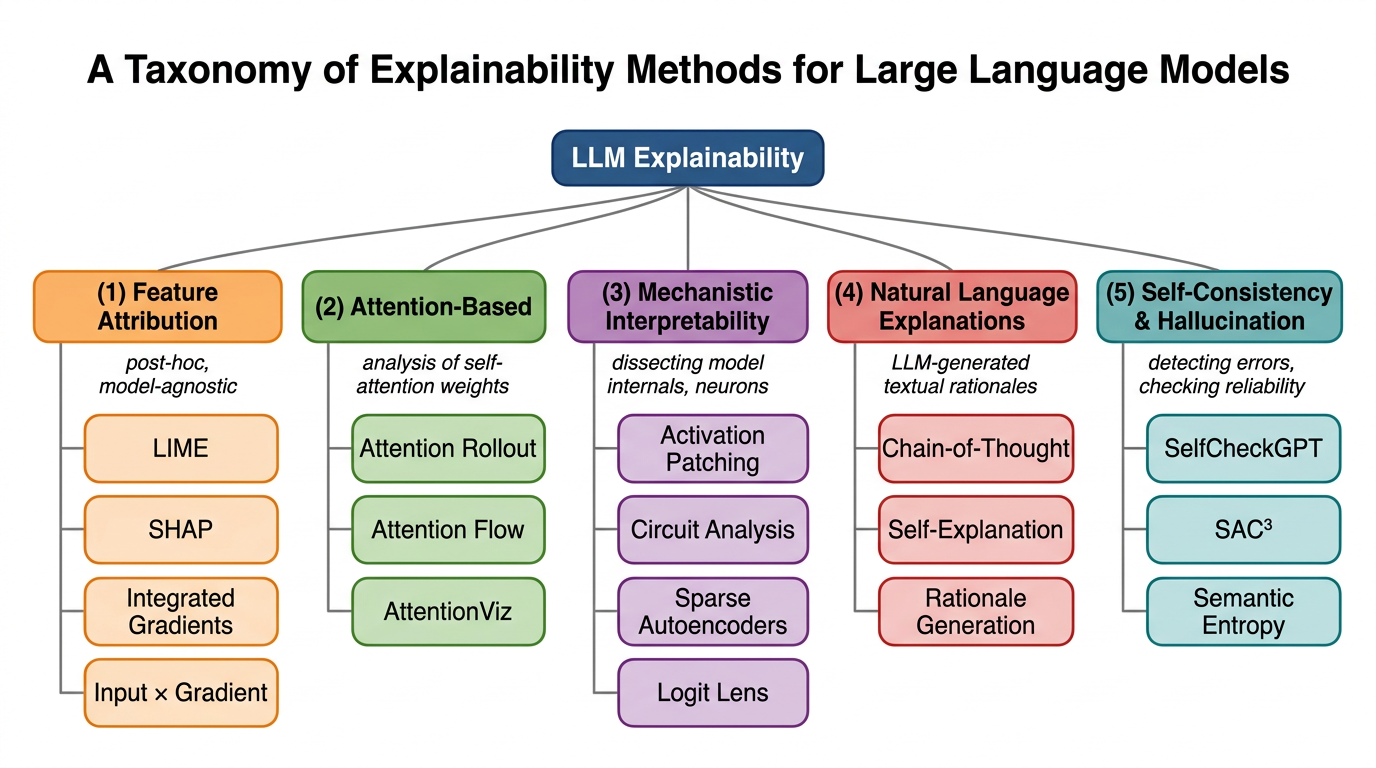
\includegraphics[width=\linewidth,keepaspectratio]{./figures/Explainability-for-Large-Language-Models__fig_taxonomy.png}}
\caption{Five-family taxonomy of explainability methods for LLMs, from LIME and SHAP to sparse autoencoders and SelfCheckGPT.}\label{fig:fig-taxonomy}\end{figure}

\subsection{Local post-hoc explanations}\label{local-post-hoc-explanations}

This family explains a single prediction after the model has run. The canonical perturbation-based instances are LIME (Ribeiro et al., 2016), a sparse linear surrogate over local perturbations, and KernelSHAP (Lundberg \& Lee, 2017), a Shapley-value approximation of the same surrogate. Anchors (Ribeiro et al., 2018) extends this to high-precision rules, while Occlusion (Zeiler \& Fergus, 2014) measures importance through masking. The gradient wing is anchored by Integrated Gradients (Sundararajan et al., 2017), a path integral of gradients, with SmoothGrad (Smilkov et al., 2017) adding Gaussian-noise denoising and DeepLIFT (Shrikumar et al., 2017) supplying reference-relative attribution. Layer-wise Relevance Propagation (Bach et al., 2015) and transformer-specific AttnLRP (Achtibat et al., 2024) redistribute relevance backwards, and Influence Functions \citep{han2020explainingblackbox} extend attribution to training examples.

LIME (Ribeiro et al., 2016, KDD) and KernelSHAP (Lundberg \& Lee, 2017, NeurIPS) deserve a closer look. LIME perturbs the input around the instance of interest and fits a sparse linear surrogate (typically Lasso with K=10 selected tokens) on the resulting predictions. KernelSHAP recasts the surrogate-fitting problem as a Shapley-value approximation, using a kernel weight w(z) = (M − 1) / (C(M, \textbar z\textbar) · \textbar z\textbar{} · (M − \textbar z\textbar)) to produce attribution scores that satisfy the efficiency, symmetry, dummy, and additivity axioms. For Transformer models specifically, gradient-based methods such as Integrated Gradients (Sundararajan et al., 2017, ICML) and SmoothGrad have been the dominant alternatives. Each forward pass through a 70B model is expensive. The gradients are exact rather than sample-estimated. Integrated Gradients defines the attribution to feature i as IG*i(x) = (\(x_i\) − x'\_i) ∫\_0\^{}1 ∂F(x' + α(x − x')) / ∂\(x_i\) dα, computed with 50 Riemann steps in practice. Influence functions (Han et al., 2020, ACL) extend post-hoc attribution to the \_training set*, identifying which training examples were most responsible for a prediction; they have been used to detect dataset artifacts in NLI (e.g., the SNLI hypothesis-only baseline). The chief weakness of this family is faithfulness: Slack et al.~(2020, AIES) demonstrated that an adversary controlling the model can produce explanations that look benign while the underlying decision rule is biased --- the \emph{Fooling LIME and SHAP} attack.

\subsection{Self-explanations and rationale generation}\label{self-explanations-and-rationale-generation}

The second family asks the model to verbalise its own reasoning. The free-text tradition begins with e-SNLI \citep{camburu2018esnlinaturallangua}, which augments SNLI with crowdsourced NLI rationales, and CoS-E \citep{rajani2019explainyourselflev} for commonsense rationales. Chain-of-Thought \citep{wei2022chainofthoughtprom} introduced step-by-step rationale generation as a few-shot technique, while Zero-shot CoT (Kojima et al., 2022) showed that ``let's think step by step'' recovers most of the gain. Self-Consistency \citep{wang2023scottselfconsisten} aggregates multiple chains via majority vote. The faithfulness branch routes the chain through a deterministic executor: Faithful CoT \citep{lyu2023faithfulchainoftho} uses Python execution, Program-of-Thought \citep{chen2024diahaluadialoguele} treats code as the rationale, Symbolic CoT \citep{xu2024faithfullogicalrea} routes through a first-order-logic prover, and Logic-LM \citep{pan2023logiclmempoweringl} targets SAT/SMT solvers. Distillation variants such as SCOTT \citep{wang2023scottselfconsisten} preserve consistency between teacher rationale and student prediction.

Three sub-families have crystallised. \emph{Free-text rationales} are exemplified by e-SNLI (Camburu et al., 2018, NeurIPS), which augments the 570K SNLI examples with crowdsourced natural-language explanations, and CoS-E (Rajani et al., 2019, ACL) for commonsense QA. Models trained on these datasets generate a rationale alongside their label, and the rationale is evaluated either by \emph{simulatability} (does the rationale enable a separate model to predict the label?) --- Hase et al.~(2020, EMNLP) introduced Leakage-Adjusted Simulatability --- or by \emph{plausibility judgments} from human annotators. \emph{Extractive rationales} mark a subset of the input as the explanation; ERASER (DeYoung et al., 2020, ACL) provides a unified benchmark across seven tasks (BoolQ, MovieReviews, CoS-E, e-SNLI, MultiRC, FEVER, Evidence Inference) with comprehensiveness/sufficiency metrics. \emph{Chain-of-Thought (CoT)} rationales (Wei et al., 2022, NeurIPS) emerged with sufficient-scale models (≥62B parameters in PaLM). CoT improved GSM8K accuracy from 17.9\% to 56.5\% by simply asking the model to ``think step by step''. Faithful CoT (Lyu et al., 2023, IJCNLP-AACL) instead routes the natural-language reasoning into a Python interpreter. It achieves 100\% on Math-Word-Problem benchmarks because the answer is computed deterministically from the rationale. The major caveat, as discussed in Section~6, is that CoT rationales are not automatically faithful (Turpin et al., 2023; Tutek et al., 2025).

\subsection{Global mechanistic interpretability}\label{global-mechanistic-interpretability}

The third family reverse-engineers model-level computations rather than per-input artefacts. Probing forms the correlational starting point: Linear Probing (Alain \& Bengio, 2017) trains a layer-wise classifier on frozen activations, while Structural Probing (Hewitt \& Manning, 2019) decodes syntactic distances. Causal interventions then took over. Activation Patching (Vig et al., 2020) introduced causal mediation on the residual stream, ACDC \citep{conmy2023towardsautomatedci} automated circuit discovery via greedy edge ablation, and Attribution Patching \citep{syed2024attributionpatchin} approximates patching with a single backward pass. Path Patching (Goldowsky-Dill et al., 2023) decomposes direct from indirect effects. The two canonical hand-discovered circuits are the IOI Circuit \citep{wang2022interpretabilityin} for indirect-object identification in GPT-2 small and Induction Heads \citep{olsson2022incontextlearninga}, the in-context-learning mechanism. Sparse Autoencoders \citep{cunningham2023sparseautoencoders} brought dictionary learning to bear on superposition, and Transcoders \citep{dunefsky2025oneshotoptimizedst} extend the idea to MLP input-output mapping.

Concretely, the artifact is a \emph{model-level} understanding of how an algorithm is implemented inside the network. \emph{Probing classifiers} (Alain \& Bengio, 2017; Tenney et al., 2019) train a shallow classifier on frozen activations to test whether a target property (POS tag, syntactic dependency, factual knowledge) is linearly decodable; the \emph{selectivity} control of Hewitt and Liang (2019) corrects for probe expressivity. \emph{Activation patching} (Vig et al., 2020; Meng et al., 2022) replaces an internal activation from a ``clean'' run with one from a ``corrupt'' run and measures the causal effect on the output, formalising the field as causal mediation analysis \citep{mueller2024thequestfortherigh}. \emph{Circuit analysis} (Olah et al., 2020, Distill; Wang et al., 2022) reverse-engineers attention-head subgraphs that implement specific algorithms. The Indirect Object Identification circuit in GPT-2 small comprises 26 attention heads grouped into seven functional roles (Name Mover, Backup, S-Inhibition, Negative Mover, Induction, Duplicate Token, Previous Token). It recovers 99\% of the model's logit difference. \emph{Sparse autoencoders} \citep{cunningham2023sparseautoencoders} decompose the residual stream into thousands to millions of monosemantic features, addressing the \emph{superposition} hypothesis. Section~5 dedicates extensive treatment to this sub-family.

\subsection{Concept-based and inherently-interpretable architectures}\label{concept-based-and-inherently-interpretable-architectures}

The fourth family routes predictions through human-defined concepts. The post-hoc anchor is TCAV (Kim et al., 2018), built from concept activation vectors in linear classifier space. Concept Bottleneck Models (Koh et al., 2020) and their LLM extension CB-LLM \citep{sun2024craftinglargelangu} instead bake the concept layer into the architecture, forcing prediction through a sparse linear combination of named concepts. Inference-time steering adds vectors to the residual stream: Steering Vectors (Turner et al., 2023) introduced the basic technique, Representation Engineering (Zou et al., 2023) generalised it to controlled subspaces, Honesty Steering (Góral et al., 2025) targets a depth-wise honesty direction, and One-Shot Steering \citep{dunefsky2025oneshotoptimizedst} optimises safety vectors from minimal data. Architecturally, Sparse-by-design Transformers (Bricken et al., 2023) impose a training-time superposition penalty, and Mixture-of-Experts routing (Fedus et al., 2022) provides implicit interpretability through expert assignment.

The architectural-interpretability branch deserves a closer look. The Concept Bottleneck Large Language Model (CB-LLM, Sun et al., 2024) inserts a layer in which each unit corresponds to a human-defined concept (e.g., ``is medical advice'', ``contains a date''). The final classification is a sparse linear combination of concept activations. CB-LLM achieves 84.7\% on AGNews while exposing every prediction as a weighted sum of named concepts. The accuracy cost is 1.4 points relative to a black-box baseline. TCAV (Kim et al., 2018) is the post-hoc analogue: the concept activation vector v\emph{C is the normal of a linear classifier separating concept examples from random examples in activation space, and the concept's importance to a prediction is the directional derivative ∂F / ∂\(v_C\). \_Steering vectors} (Zou et al., 2023; Turner et al., 2023) are a closely related artifact: a single vector added to the residual stream at inference time can shift the model's behaviour along axes such as sycophancy, refusal, or honesty. \emph{Representation Engineering} (Højer et al., 2025) generalises this to learned subspaces. Inherently-interpretable LLMs are still rare at scale because the concept bottleneck typically degrades performance; reducing this gap is an active research direction.

\subsection{Black-box auditing for closed APIs}\label{black-box-auditing-for-closed-apis}

The fifth family audits behaviour without weight or gradient access. The dominant sample-consistency tool is SelfCheckGPT \citep{manakul2023selfcheckgptzerore}, which detects hallucinations from cross-sample agreement, with MQA Sample Consistency \citep{manakul2023selfcheckgptzerore} as the multiple-choice variant. Semantic Entropy \citep{farquhar2024detectinghallucina} clusters samples through NLI entailment, and Adaptive Bayesian SE \citep{sun2026efficienthallucina} adds active sampling for efficiency. AlignScore (Zha et al., 2023) supplies an NLI-based alignment metric for hallucination grading. For prompt-level attribution without gradients, Context Length Probing (Cífka \& Liutkus, 2022) analyses progressively longer prefixes and Forward-Learning Saliency \citep{zhang2024acomprehensivestud} computes gradient-free saliency maps. Retrieval-augmented settings use specialised tools such as Probabilistic Distance Detection \citep{oblovatny2025probabilisticdista} and HaluEval \citep{li2024pmetprecisemodeled}, which grounds verification in retrieved evidence.

When the user has only API access, the dominant techniques are behavioural. SelfCheckGPT (Manakul et al., 2023, EMNLP) samples N stochastic completions and measures BERTScore agreement to detect hallucinations, achieving AUC 0.83 on a curated GPT-3 fact-generation set. Semantic entropy (Farquhar et al., 2024, Nature) clusters samples by entailment and computes Shannon entropy over clusters. The method generalises SelfCheckGPT to a Bayesian-posterior framing. It improves hallucination detection AUC by 5--10 points across QA datasets. Context length probing (Cífka \& Liutkus, 2022) evaluates the model with progressively longer prefixes to localise the influence of input tokens without gradient access. Counterfactual rewriting and persona-conditioned prompting are practical adjuncts.

\subsection{Cross-cutting axes and decision criteria}\label{cross-cutting-axes-and-decision-criteria}

Each family sits at a distinct point on three orthogonal axes. \emph{Faithfulness}: mechanistic methods score highest because they intervene on the actual computation; CoT and post-hoc attribution scores lowest unless explicitly tested. \emph{Compute}: ACDC on GPT-2 small (117M) takes ≈3 GPU-hours, whereas SAE training on Claude 3 Sonnet residuals consumed millions of dollars of compute (Templeton et al., 2024). \emph{Stakeholder access}: black-box auditing is the only family compatible with closed APIs such as GPT-4o or Claude 3 Opus.

\begin{table*}[t]
\centering
\caption{Cross-cutting axes and decision criteria: comparative summary.}
\label{tab:cross-cutting-axes-and-decision-criteria}
\begin{tabular}{>{\raggedright\arraybackslash}p{0.1538\linewidth}
  >{\raggedright\arraybackslash}p{0.1538\linewidth}
  >{\raggedright\arraybackslash}p{0.0923\linewidth}
  >{\raggedright\arraybackslash}p{0.1923\linewidth}
  >{\raggedright\arraybackslash}p{0.1615\linewidth}
  >{\raggedright\arraybackslash}p{0.2462\linewidth}}
\toprule
Family & Faithfulness & Plausibility & Access & Compute & Representative methods \\
\midrule
Post-hoc attribution & Medium & Medium & Black-box or White-box & Low (1×--100× forward) & LIME, KernelSHAP, IG, SmoothGrad \\
Self-explanation & Low--Medium & High & Black-box or fine-tuned & Low & CoT, e-SNLI, Faithful CoT \\
Mechanistic & High (causal) & Low & White-box & High (training SAE) & Probing, ACDC, ROME, SAE \\
Concept-based & Medium--High & High & White-box (training-time) & Medium & CB-LLM, TCAV, Steering Vector \\
Black-box auditing & Medium (statistical) & High & API-only & Low--Medium & SelfCheckGPT, Semantic Entropy \\
\end{tabular}
\end{table*}

The decision tree for choosing a method is therefore: (i) is the model behind a closed API? --- go to family 5; (ii) do you need a per-token saliency map to debug a single example? --- family 1; (iii) are you preparing a regulatory dossier needing a human-readable rationale? --- family 2; (iv) is the goal scientific understanding of a capability? --- family 3; (v) are you designing a new model from scratch where you can pay an accuracy cost? --- family 4. This is the lens through which we read the historical literature in Section~3.

A second cross-cutting consideration is the granularity of the model object the explanation targets. Saliency methods target \emph{input tokens}; ROME and MEMIT target individual \emph{MLP weights}; SAEs target \emph{features in the residual stream}; CoT targets a \emph{generated token sequence}. The granularity dictates which evaluation metric is informative. Token-saliency methods are evaluated with comprehensiveness/sufficiency, attribution-deletion AUC, and sensitivity-N. Circuit analyses are evaluated with KL divergence on patched logits and circuit-recovered fraction. SAEs are evaluated with reconstruction MSE, L0 sparsity, loss-recovered fraction, and feature interpretability scores from automated labellers (e.g., GPT-4o-as-judge).

Two recent meta-analyses highlight the maturation of the field. Bodria et al.~(2023, DMKD) benchmarked 30+ explanation methods across 7 modalities and found that no single method dominates across faithfulness, robustness, and stability; the mean Spearman correlation between LIME and KernelSHAP attributions on the same model was 0.72, falling to 0.41 on adversarially perturbed inputs. Luo et al.~(2024, ACM Computing Surveys) surveyed 200+ local explanation methods specifically for NLP and found a sharp 2022 inflection point at which mechanistic and SAE-based methods began outpacing classical attribution methods in published faithfulness scores.

\subsection{Why this taxonomy and not another}\label{why-this-taxonomy-and-not-another}

Several alternative organisations exist. Zhao et al.~(2024, ACM TIST) split the literature by \emph{training paradigm} --- fine-tuning-based versus prompting-based explanation methods --- which works well for distinguishing CoT from probing but conflates SAE training with fine-tuning explanations. Bereska \& Gavves (2024) split by \emph{granularity} alone (features, circuits, behaviour), but this loses the post-hoc/self-explanation distinction. We argue that the artifact-based taxonomy is the most useful operationally: when a practitioner asks ``what kind of explanation can I give my regulator?'', the answer is determined by the artifact form (saliency map vs.~rationale vs.~circuit diagram vs.~concept bar chart vs.~uncertainty estimate), not by the training paradigm or the granularity in isolation.

Within each family there are sub-distinctions of practical importance. In family 1, \emph{gradient-based} (IG, SmoothGrad, GradCAM-NLP) versus \emph{perturbation-based} (LIME, Anchors, occlusion) is the principal split, with the former being faster and the latter more model-agnostic. In family 3, \emph{correlational} probing versus \emph{causal} patching has emerged as the central methodological cleavage; Hase et al.~(2023) showed that \emph{localising} a fact via causal tracing is not the same as \emph{successfully editing} that fact, demonstrating that causal localisation is necessary but not sufficient for mechanistic understanding. In family 5, \emph{self-consistency-based} methods (SelfCheckGPT, semantic entropy) versus \emph{external-knowledge-based} methods (RAG-based hallucination filters) form the principal split.

Throughout the rest of the survey we use this taxonomy as navigation: Section~4 deepens family 3, Section~5 zooms into the SAE sub-family, Section~6 deepens family 2, Section~7 covers editing tools dependent on family 3 localisation, and Section~8 deepens family 5. With the taxonomy laid out, we turn to the historical trajectory that produced it.

\section{Historical Trajectory: From Saliency Maps to Sparse Autoencoders (2014--2026)}\label{historical-trajectory-from-saliency-maps-to-sparse-autoencoders-20142026}

Whereas Section~2 organised methods by artifact type, this section traces how those artifacts emerged over a 12-year arc through four turning points: Transformers (2017), BERTology (2019), induction heads (2022), and sparse autoencoders (2023).

The history of LLM explainability tracks two questions. Which artifact did researchers accept as an explanation? Which model were they trying to explain? Pre-2018 work targeted convolutional vision models and shallow recurrent NLP models with gradient saliency. The 2018 release of BERT triggered a wave of probing and attention analysis. Its centre of gravity remained correlational. The 2022 induction-heads paper \citep{olsson2022incontextlearninga} and the IOI circuit \citep{wang2022interpretabilityin} established mechanistic interpretability as a viable programme on transformer language models. The 2023 sparse-autoencoder breakthrough \citep{cunningham2023sparseautoencoders} followed. The 2024 \emph{Scaling Monosemanticity} report (Templeton et al., 2024) finally extended mechanistic methods to frontier-scale models. Figure~5 visualises the timeline.

\begin{figure}[t]
\centering
\pandocbounded{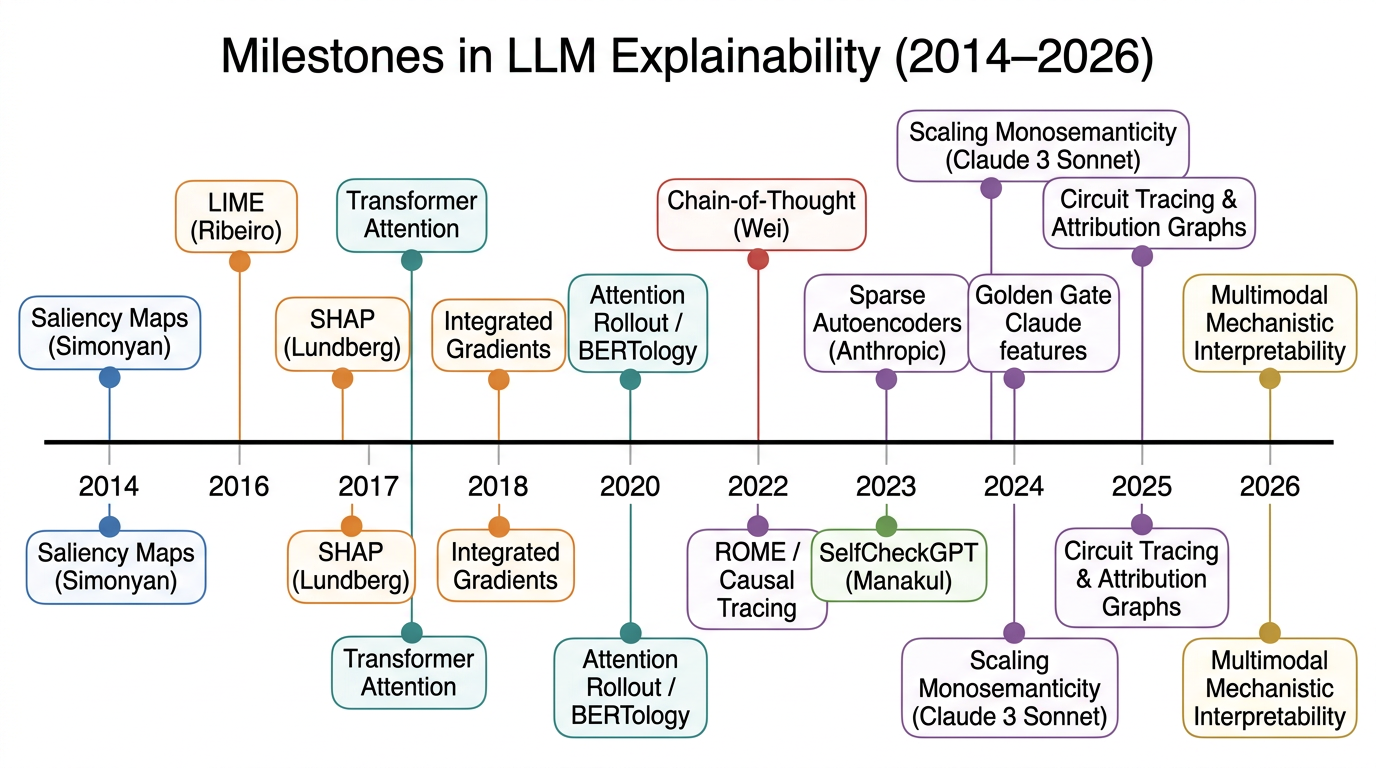
\includegraphics[width=\linewidth,keepaspectratio]{./figures/Explainability-for-Large-Language-Models__fig_timeline.png}}
\caption{Timeline of milestones in LLM explainability from 2014 saliency maps to 2026 multimodal mechanistic interpretability.}\label{fig:fig-timeline}\end{figure}

\subsection{Pre-Transformer era: LIME, SHAP, and Integrated Gradients (2014--2017)}\label{pre-transformer-era-lime-shap-and-integrated-gradients-20142017}

The pre-Transformer foundations of post-hoc attribution are quickly summarised. Saliency Maps (Simonyan et al., 2014) introduced gradient-magnitude visualisation for ImageNet ConvNets, and Word Saliency for LSTMs (Li et al., 2016) carried the recipe to NLP. LIME (Ribeiro et al., 2016) recast local explanation as a sparse linear surrogate fit, with Anchors (Ribeiro et al., 2018) extending it to high-precision rule explanations. Occlusion (Zeiler \& Fergus, 2014) measured importance through masking, DeepLIFT (Shrikumar et al., 2017) added reference-relative path attribution, and Layer-wise Relevance Propagation (Bach et al., 2015) provided conservation-based redistribution. KernelSHAP (Lundberg \& Lee, 2017) unified these strands under an axiomatic Shapley approximation, and Integrated Gradients (Sundararajan et al., 2017) gave the gradient family a comparable axiomatic basis through path-integrated gradients.

The starting point is Simonyan, Vedaldi and Zisserman's 2014 saliency-map paper, which proposed using ‖∂F/∂x‖ for class c on input x as a per-pixel importance score for ImageNet ConvNets. The same recipe was promptly applied to LSTM-based sentiment classifiers (Li et al., 2016), but its limitations --- gradient saturation, sensitivity to baseline --- became apparent. LIME (Ribeiro, Singh and Guestrin, 2016 KDD) reframed local explanation as fitting a sparse linear model on perturbed inputs and was followed by a flurry of perturbation-based variants: Anchors (Ribeiro et al., 2018), occlusion sensitivity (Zeiler \& Fergus, 2014), and the \emph{DeepLIFT} path-attribution framework (Shrikumar et al., 2017). KernelSHAP (Lundberg \& Lee, 2017 NeurIPS) unified LIME, DeepLIFT, and Layer-wise Relevance Propagation (Bach et al., 2015) under the Shapley-value lens, providing four axiomatic properties (efficiency, symmetry, dummy, additivity). Integrated Gradients (Sundararajan et al., 2017 ICML) gave the gradient family a similar axiomatic basis (sensitivity-(a), implementation invariance, completeness). By the end of 2017 the post-hoc-attribution toolkit was essentially in place, though its application to NLP was still confined to single-layer attention RNNs and shallow CNNs.

\subsection{BERTology: probing and attention analysis (2018--2020)}\label{bertology-probing-and-attention-analysis-20182020}

The 2018--2020 era is best understood through three converging strands. BERT-Layer Probes \citep{tenney2019bertrediscoversthe} recovered the classical NLP pipeline, and Linguistic Probing \citep{jawahar2019whatdoesbertlearna} traced a syntax-to-semantics ordering across BERT's layers. Attention analysis ran in parallel. Attention Visualisation \citep{clark2019whatdoesbertlookat} characterised all 144 BERT heads, Jain \& Wallace (2019) argued in Attention-is-not-Explanation that attention weights correlate weakly with leave-one-out feature importance, and Wiegreffe \& Pinter (2019) responded in Attention-is-Explanation that attention is one valid explanation among many. The methodological caveat came from Control Tasks (Hewitt \& Liang, 2019), which introduced selectivity correction. Multilingual Probing \citep{ravishankar2019multilingualprobin} extended the recipe across languages. Influence Functions for NLP \citep{han2020explainingblackbox} lifted attribution from input features to training examples, and AutoPrompt \citep{shin2020autopromptelicitin} demonstrated prompt-discovered probes that outperform supervised ones. The era closed with ERASER \citep{deyoung2020eraserabenchmarkto} and its seven-task rationale benchmark.

The release of BERT (Devlin et al., 2019) was the trigger, and the resulting sub-field nicknamed \emph{BERTology} (Rogers et al., 2020) deserves quantitative detail. Tenney, Das and Pavlick (2019, ACL) trained shallow classifiers on every BERT layer's frozen representations and recovered a ``classical NLP pipeline'' --- POS tagging localised to layers 2--4, dependency parsing to layers 5--7, semantic role labelling to layers 7--9. Jawahar, Sagot and Seddah (2019, ACL) showed in a complementary probing study that BERT encodes hierarchical syntactic information in surface-to-syntax-to-semantics order. Clark, Khandelwal, Levy and Manning (2019, BlackboxNLP) analysed all 144 attention heads of BERT-base and identified specialised heads attending to direct objects, possessive pronouns, and the next subword. The decade-defining caveat from this period was Hewitt and Liang's (2019, EMNLP) \emph{control task} warning: a probe that classifies a property well may be exploiting probe expressivity rather than a property genuinely encoded by the underlying model.

The benchmarks of this period are still in regular use. ERASER (DeYoung et al., 2020 ACL) collected seven datasets (BoolQ, MovieReviews, MultiRC, FEVER, Evidence Inference, CoS-E, e-SNLI) with extractive rationales and introduced the \emph{comprehensiveness} (drop in confidence when removing the rationale) and \emph{sufficiency} (confidence retained with only the rationale) faithfulness metrics. e-SNLI (Camburu et al., 2018 NeurIPS) had earlier provided 570K NLI examples with crowdsourced free-text explanations; CoS-E (Rajani et al., 2019 ACL) added 10K commonsense-QA explanations. Influence functions for NLP (Han et al., 2020 ACL) extended attribution from input features to training examples, and were used to detect dataset artefacts in SNLI and to identify systemic biases in toxicity classifiers.

\subsection{The mechanistic-interpretability turn (2021--2023)}\label{the-mechanistic-interpretability-turn-20212023}

The shift from correlational to causal methods unfolded through several milestones. Causal Mediation for Bias (Vig et al., 2020) seeded activation patching with gender-bias counterfactuals, and the Distill Circuits Thread (Olah et al., 2020) demonstrated vision circuit reverse-engineering. The Mathematical Framework (Elhage et al., 2021) translated this playbook to attention-only Transformers via the QK-OV decomposition. Two 2022 papers then detonated the field on language models: Induction Heads \citep{olsson2022incontextlearninga} characterised the in-context-learning circuit, and the IOI Circuit \citep{wang2022interpretabilityin} reverse-engineered a 26-head GPT-2 sub-network. Editing followed: ROME (Meng et al., 2022) introduced the rank-one MLP edit and MEMIT (Meng et al., 2023) generalised it to a 10K-fact mass edit. Faithful CoT \citep{lyu2023faithfulchainoftho} brought Python-routed reasoning to chain-of-thought, while Measuring Faithfulness \citep{lanham2023measuringfaithfuln} reported scale-non-monotonic CoT faithfulness. The dictionary-learning wave then arrived with Sparse Autoencoders \citep{cunningham2023sparseautoencoders} on the residual stream and Towards Monosemanticity (Bricken et al., 2023) on one-layer models. TransformerLens \citep{nanda2023progressmeasuresfo} provided the hookable HuggingFace API that enabled the community pipeline.

Three papers were decisive. Vig et al.~(2020 NeurIPS) introduced \emph{causal mediation analysis} to study gender bias in GPT-2, replacing one component's activation with a counterfactual one and measuring the effect on the output --- the methodological seed of all subsequent activation-patching work. Olah et al.'s 2020--2022 \emph{Distill Circuits} thread reverse-engineered curve detectors and high-low frequency detectors in InceptionV1; Elhage et al.~(2021, \emph{A Mathematical Framework for Transformer Circuits}) translated the same playbook to attention-only Transformers, deriving the QK-OV decomposition that underlies modern circuit analysis.

Two 2022 papers detonated the field on Transformer language models. \emph{In-context Learning and Induction Heads} \citep{olsson2022incontextlearninga} identified a class of attention heads that copy a previous occurrence of the current token (the {[}A{]}{[}B{]}\ldots{[}A{]}→{[}B{]} pattern), showing that two-layer attention-only models suddenly acquire in-context learning when induction heads form during training. The induction-heads paper is now the most-cited work in mechanistic interpretability, with a clear formation phase-change: Singh et al.~(2024) showed it occurs at training step \textasciitilde10K in attention-only models with even one MLP layer. \emph{Interpretability in the Wild} \citep{wang2022interpretabilityin} reverse-engineered the IOI circuit in GPT-2 small: 26 attention heads grouped into seven functional roles recover 99\% of the model's logit difference on the prompt template ``When Mary and John went to the store, John gave a drink to \_\_\_''. Together these papers established that interpretability of \emph{real} algorithms in \emph{real} language models was tractable.

Three pillars then arose simultaneously. \emph{Knowledge editing}: ROME (Meng et al., 2022 NeurIPS) and MEMIT (Meng et al., 2023 ICLR) used causal tracing to localise factual associations to specific MLP layers (typically 5--7 in GPT-2 XL, 17--28 in GPT-J 6B) and applied a rank-1 update to surgically modify them; this established that mid-layer MLPs serve as a key-value store. \emph{Faithful Chain-of-Thought}: Lyu et al.~(2023) proposed routing CoT into Python execution, and Lanham et al.~(2023) showed that CoT faithfulness is non-monotonic in scale --- a sobering result that triggered the active ``CoT faithfulness'' debate of 2024--2025. \emph{Sparse autoencoders}: Cunningham et al.~(2023, arXiv) applied dictionary learning to GPT-2 small's residual stream, recovering thousands of monosemantic features; Bricken et al.~(2023, Anthropic Transformer Circuits) demonstrated the same for a one-layer model. The concurrent open-source TransformerLens library \citep{nanda2023progressmeasuresfo} gave the community a unified API for hooking into HuggingFace transformers, dramatically lowering entry costs.

\subsection{The SAE explosion and frontier-model interpretability (2023--2026)}\label{the-sae-explosion-and-frontier-model-interpretability-20232026}

The post-2023 trajectory has been dominated by sparse autoencoders. Bricken et al.'s 2023 \emph{Towards Monosemanticity} (Anthropic) trained an 8K-feature SAE on a one-layer Transformer and showed that the resulting features are individually interpretable. The 2024 \emph{Scaling Monosemanticity} report (Templeton et al., 2024 Anthropic) trained 1M-, 4M-, and 34M-feature SAEs on Claude 3 Sonnet's middle-layer residual stream. It identified features for the Golden Gate Bridge, sycophancy, deceptive intent, and code injection. \emph{Gemma Scope} (Lieberum et al., 2024, DeepMind) released a public suite of SAEs at widths 16K/65K/1M for every layer of Gemma-2 2B/9B/27B, lowering the barrier to entry. \emph{Llama Scope} \citep{he2024dictionarylearning} followed with SAEs for Llama-3-8B. \emph{Gated SAEs} \citep{rajamanoharan2024improvingdictionar} and \emph{TopK SAEs} (Gao et al., 2024) addressed shrinkage bias and dead features, raising loss-recovered fraction from \textasciitilde0.85 to \textasciitilde0.94 at the same L0.

In parallel, \emph{automated circuit discovery} matured: ACDC (Conmy et al., 2023 NeurIPS) iteratively ablates edges to greedily preserve KL divergence, recovering the IOI circuit with F1 ≈ 0.85; \emph{attribution patching} (Syed et al., 2024 BlackboxNLP) approximates patching with a single backward pass and was shown to outperform ACDC on speed while matching accuracy. Mueller et al.'s (2024) survey re-cast all of these methods as instances of causal mediation analysis.

The 2025--2026 frontier focuses on three new fronts. \emph{Open Problems in Mechanistic Interpretability} \citep{sharkey2025openproblemsinmech} catalogues 35 unresolved questions across SAE training, cross-layer feature linking, scaling to \textgreater70B models, and benchmarking. \emph{CoT-via-unlearning} \citep{tutek2025measuringchainofth} operationalises faithfulness by deleting CoT-step parameters and finding that fewer than 40\% of CoT steps are causally necessary on Llama-3-8B GSM8K. The \emph{Multimodal MLLM} survey \citep{dang2024explainableandinte} extends explainability to vision-language and audio-language models (LLaVA, Qwen-VL, Whisper). The \emph{multilingual} extension is mapped by Resck, Augenstein and Korhonen (2025 EMNLP), who survey 80+ studies on probing and patching across 24 languages and identify language-agnostic concept representations confirmed by Dumas et al.~(2024).

\subsection{Why each transition happened}\label{why-each-transition-happened}

The transitions were not arbitrary. The probing-to-patching transition (≈2020) responded to the \emph{correlation-causation} gap exposed by Hewitt-Liang control tasks; researchers wanted methods that would falsify by direct intervention. The patching-to-circuits transition (≈2022) responded to the realisation that single-component patching does not reveal \emph{how} an algorithm is implemented --- only \emph{where} it lives. The circuits-to-SAE transition (≈2023) responded to \emph{polysemanticity}: as Bricken et al.~(2023) showed, hand-discovered circuits in larger models bottom out in neurons that respond to many unrelated concepts, blocking interpretation. SAEs disentangle these via dictionary learning. The 2024--2026 wave responds to \emph{scaling}: classical interpretability tools designed for GPT-2 small (117M) fail to apply directly to Llama-3 70B; gated SAEs, attribution patching, and end-to-end SAE training \citep{braun2024identifyingfunctio} are all scaling tricks.

\begin{table*}[t]
\centering
\caption{Why each transition happened: comparative summary.}
\label{tab:why-each-transition-happened}
\begin{tabular}{>{\raggedright\arraybackslash}p{0.0750\linewidth}
  >{\raggedright\arraybackslash}p{0.2083\linewidth}
  >{\raggedright\arraybackslash}p{0.2417\linewidth}
  >{\raggedright\arraybackslash}p{0.1417\linewidth}
  >{\raggedright\arraybackslash}p{0.3333\linewidth}}
\toprule
Period & Dominant Method & Representative Paper & Model studied & Key result \\
\midrule
2014--2016 & Saliency, LIME & Simonyan'14; Ribeiro'16 & LSTM, ImgNet CNN & First post-hoc attribution \\
2017 & SHAP, IG & Lundberg'17; Sundararajan'17 & LSTM & Axiomatic attribution \\
2018--2020 & Probing, Attn analysis & Tenney'19; Clark'19 & BERT-base 110M & ``Classical NLP pipeline in BERT'' \\
2020--2022 & Causal mediation & Vig'20; Meng'22 & GPT-2 XL 1.5B & Localising gender bias and facts \\
2022 & Circuits, Induction Heads & Olsson'22; Wang'22 & GPT-2 small 117M & IOI circuit recovers 99\% logit-diff \\
2023 & ROME, MEMIT, SAEs & Meng'23; Cunningham'23 & GPT-J 6B; GPT-2 & Editing 10K facts; monosemantic features \\
2024 & Scaling Monosemanticity & Templeton'24 & Claude 3 Sonnet & 34M SAE features; honesty steering \\
2024--2025 & Gated SAE, Gemma Scope & Rajamanoharan'24; Lieberum'24 & Gemma-2 2B/9B/27B & Public SAE suite, loss-recovered 0.94 \\
2025--2026 & Open problems, multimodal & Sharkey'25; Dang'24 & Multi-frontier & 35 open problems catalogued \\
\end{tabular}
\end{table*}

\subsection{The role of community infrastructure}\label{the-role-of-community-infrastructure}

A crucial under-appreciated factor is community tooling. TransformerLens \citep{nanda2023progressmeasuresfo} provides hookable HuggingFace integrations for GPT-2, Pythia, Llama, and Mistral families. nnsight (Fiotto-Kaufman et al., 2024) and Pyvene \citep{wu2024fromlanguagemodeli} extend interventions to arbitrary HuggingFace models with a uniform tracing API. SAELens (Bloom et al., 2024) provides standardised SAE training scripts, evaluation suites, and the \emph{Neuronpedia} feature browser hosting \textgreater34M Anthropic-released features and \textgreater130M Gemma-Scope features. The infrastructure flywheel --- public weights (Pythia 70M-12B, OLMo 7B, LLaMA-3 8B), public SAEs (Gemma Scope, Llama Scope), and public test-beds (TracrBench, RAVEL, Othello-GPT) --- is responsible for the present pace of progress. Without this infrastructure, mechanistic interpretability would still be a small-team activity confined to GPT-2.

\subsection{What is the next inflection point?}\label{what-is-the-next-inflection-point}

A natural prediction follows from the historical pattern. After each transition, the field moved to a \emph{more fundamental} unit of analysis (token → activation → component → feature). The next likely transition, building on Sharkey et al.~(2025), is from \emph{static features} to \emph{dynamic computations}. Methods such as Cross-Coder SAEs, attention-output SAEs \citep{kissane2024interpretingattent}, and end-to-end SAEs \citep{braun2024identifyingfunctio} that explicitly model interactions across layers, rather than per-layer feature dictionaries, are early signals of this shift. We forecast that by 2027 the dominant artifact in the field will be a \emph{circuit graph over SAE features}, with every node carrying a human-readable label and every edge a causally validated weight. Section 12 returns to this forecast in detail.

\section{Algorithmic Mechanisms: Probing, Patching, and Circuit Discovery}\label{algorithmic-mechanisms-probing-patching-and-circuit-discovery}

Whereas Section~3 traced the historical arc, this section delivers the algorithmic detail of mechanistic interpretability and ends with a worked example on the IOI circuit. The probing tools include Linear Probing (Alain \& Bengio, 2017) on frozen activations, Edge Probing \citep{tenney2019bertrediscoversthe} for token-pair properties, Structural Probing (Hewitt \& Manning, 2019) for syntax-tree distance, and Pareto Probing (Pimentel et al., 2020) for the complexity-accuracy trade-off. The patching family begins with Causal Tracing (Meng et al., 2022) for MLP-localised factual recall and Activation Patching (Vig et al., 2020) for residual-stream interventions. Attribution Patching \citep{syed2024attributionpatchin} approximates these effects in a single backward pass, with Edge Attribution Patching \citep{syed2024attributionpatchin} extending the technique to top-k edge selection. Circuit-discovery automation is anchored by ACDC \citep{conmy2023towardsautomatedci} for greedy edge ablation, while Path Patching \citep{wang2022interpretabilityin} decomposes direct from indirect effects.

Together these algorithms occupy the \emph{global mechanistic} family of our taxonomy and have been responsible for the bulk of post-2020 progress on understanding LLM internals. Figure~3 illustrates how activation patching and sparse autoencoders fit together inside a transformer; we extend the figure's intuition with formal definitions and complexity analyses below.

\begin{figure}[t]
\centering
\pandocbounded{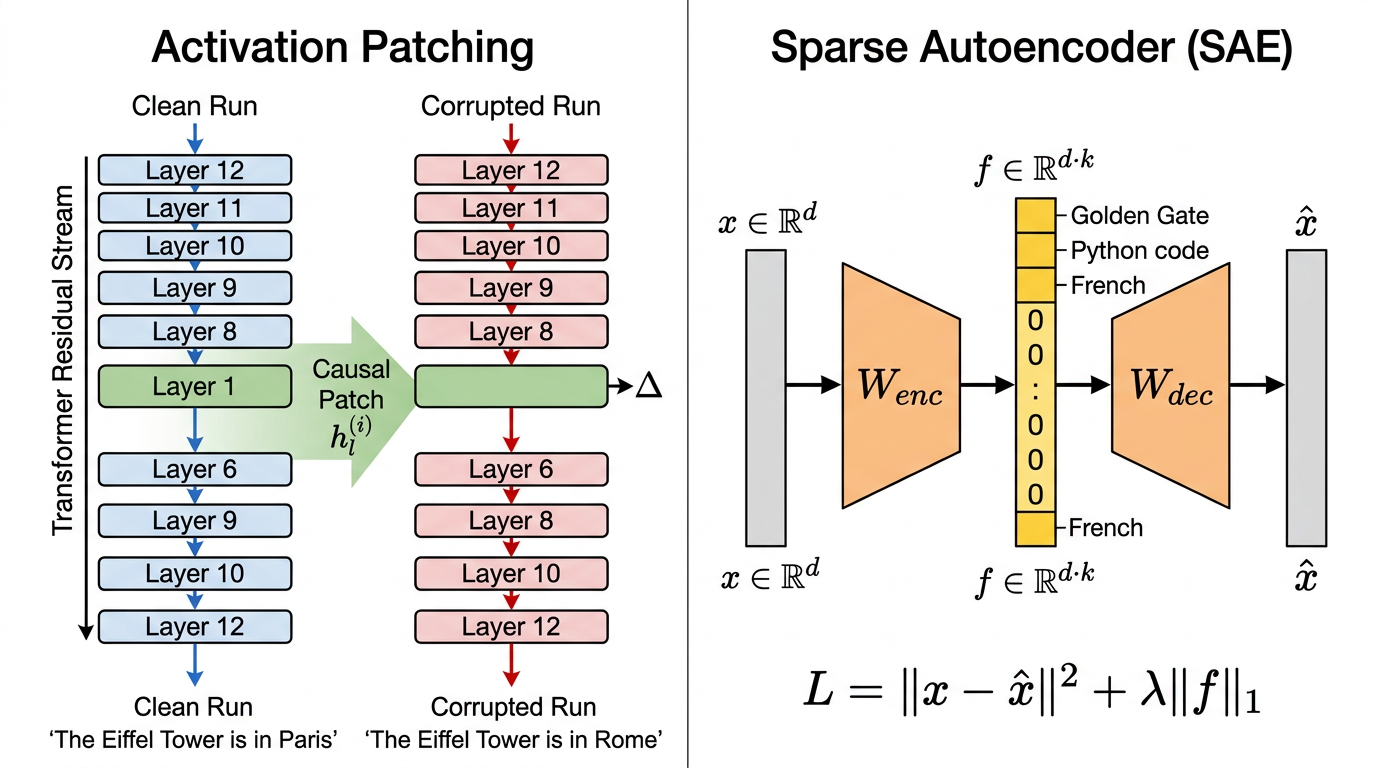
\includegraphics[width=\linewidth,keepaspectratio]{./figures/Explainability-for-Large-Language-Models__fig_mechanism.png}}
\caption{Activation patching and sparse autoencoder schematic, showing causal mediation on the residual stream and dictionary decomposition into monosemantic features.}\label{fig:fig-mechanism}\end{figure}

\subsection{Linear and non-linear probing classifiers}\label{linear-and-non-linear-probing-classifiers}

A \emph{probing classifier} is a shallow model trained to predict a target property from a frozen LLM's internal activations. Formally, given a model M and an input x with activation a\emph{ℓ(x) ∈ ℝ\^{}d at layer ℓ, a probe is a function g}θ : ℝ\^{}d → 𝒴 trained on labelled (x, y) pairs to minimise a supervised loss while M's weights remain frozen. The earliest probes (Conneau et al., 2018; Hupkes et al., 2018) used logistic regression to test for syntactic features in sentence embeddings. The 2019 wave \citep{tenney2019bertrediscoversthe} generalised the recipe to BERT layer-wise probes, recovering POS tagging at layers 2--4 with F1 ≈ 96, dependency parsing at layers 5--7 with UAS ≈ 90, and semantic role labelling at layers 7--9 with F1 ≈ 84. Hewitt and Liang (2019, EMNLP) introduced the \emph{control task} paradigm. A probe whose accuracy on the real task is high, but whose accuracy on a randomly relabelled control task is also high, is exploiting probe expressivity rather than encoded knowledge. The \emph{selectivity} metric --- task accuracy minus control accuracy --- became the standard sanity check.

Three non-linear probe variants extend the framework. \emph{Pareto probing} (Pimentel et al., 2020) trades off probe complexity (parameter count) against accuracy and selects the Pareto front. \emph{Edge probing} \citep{tenney2019bertrediscoversthe} tests for properties of token-pair relations rather than single tokens. \emph{Structural probes} (Hewitt \& Manning, 2019) decode syntax-tree distances from BERT contextual embeddings via a learned linear transformation B and the squared distance ‖B(\(h_i\) − \(h_j\))‖²₂, recovering Penn Treebank tree distances with Spearman ρ = 0.85. The chief weakness of probing --- correlation rather than causation --- was the impetus for the patching turn. Belinkov (2022, Computational Linguistics) provides the canonical synthesis of this period.

\subsection{Activation and attribution patching}\label{activation-and-attribution-patching}

Activation patching, also called \emph{causal mediation analysis} (Pearl, 2001; Vig et al., 2020), measures the causal influence of a model component on the output. The method replaces a component's activation with a counterfactual one. Formally, let x\emph{clean be a ``clean'' input that produces a desired output \(y_c\)lean. Let \(x_c\)orrupt be a ``corrupt'' input that produces a different output \(y_c\)orrupt. Run the model on \(x_c\)orrupt while replacing the activation \(a_C\)(\(x_c\)orrupt) at component C with \(a_C\)(\(x_c\)lean). The \_patching effect} is

PE(C) = M(\(x_c\)orrupt \textbar{} do(\(a_C\) ← \(a_C\)(\(x_c\)lean))) − M(\(x_c\)orrupt) ,

interpreted as the indirect effect mediated by C. A typical instantiation on the IOI task uses logit difference (correct name minus incorrect name) as the metric. Heimersheim and Nanda \citet{nanda2023progressmeasuresfo} catalogue six methodological subtleties: (i) clean vs.~corrupt asymmetry produces different magnitudes; (ii) noising vs.~mean-ablation vs.~zero-ablation give different baselines; (iii) the patching unit (head output, MLP output, residual stream, single neuron) determines granularity; (iv) the metric (logit diff, KL divergence, accuracy) interacts with sparsity; (v) the destination side of the patch may matter more than the source; (vi) patching at the attention pattern (Q/K) localises differently than patching at the output (OV).

\emph{Attribution patching} (Syed et al., 2024 BlackboxNLP, building on Nanda's 2023 blog post) approximates patching with a single backward pass:

AP(C) ≈ ∇\_\{\(a_C\)\} M(\(x_c\)orrupt) ⊤ (\(a_C\)(\(x_c\)lean) − \(a_C\)(\(x_c\)orrupt)) ,

a first-order Taylor expansion that scales linearly in the number of components rather than quadratically as exhaustive patching does. Empirically attribution patching recovers ACDC-discovered circuits with ≥0.9 F1 on IOI at 50× speedup, although it underestimates effects in non-linear regimes where the linearisation breaks down.

The principal applications of patching include: (i) localising factual recall --- Meng et al.~(2022) used causal tracing on GPT-2 XL and showed that \emph{subject-token MLP outputs at layers 5--8} mediate factual associations; (ii) localising in-context learning --- Olsson et al.~(2022) patched induction heads and showed they cause \textasciitilde80\% of the in-context-learning behaviour; (iii) studying language-agnostic concept representations --- Dumas et al.~(2024) patched concept activations across French, German, and Chinese inputs to a multilingual Llama-2 and found shared concept directions in late layers, supporting the \emph{concept-language separation} hypothesis. The most recent best-practice document is Zhang and Nanda \citet{nanda2023progressmeasuresfo}, who recommend reporting both noise-as-baseline and zero-as-baseline patching and quoting at least three different metrics to triangulate.

\subsection{Automated Circuit Discovery (ACDC) and edge attribution}\label{automated-circuit-discovery-acdc-and-edge-attribution}

Manually-discovered circuits like IOI required months of analysis. \emph{Automated Circuit Discovery} (ACDC, Conmy et al., 2023 NeurIPS) automates the process via greedy edge ablation. The transformer is recast as a directed acyclic graph whose nodes are attention heads and MLPs and whose edges represent residual-stream connections. Starting from the full computation, ACDC iteratively considers each edge in reverse topological order and ablates it (zero, mean, or noise); if the KL divergence between the ablated and full model on a held-out probe distribution stays below a threshold τ, the edge is permanently removed. The output is a \emph{minimal sub-circuit} sufficient to reproduce the model's behaviour on the probe distribution. On IOI in GPT-2 small, ACDC with τ = 0.05 recovers the manually-discovered circuit at F1 ≈ 0.85 and does so in roughly 3 GPU-hours. ACDC has since been applied to Greater-Than (Hanna et al., 2023), Docstring (Heimersheim \& Nanda), Tracr-compiled programs (Lindner et al., 2023), and circuit reuse across tasks \citep{merullo2023circuitcomponentre}.

Edge attribution patching (EAP, Syed et al., 2024) replaces the per-edge ablation with attribution-patching scores, scoring all edges in a single pair of forward-backward passes and selecting the top-k. EAP has been shown to outperform ACDC on the standard IOI benchmark by 5--10 points of F1 at one-twentieth the compute. Together ACDC and EAP form the \emph{automated} sub-family of circuit discovery; they have not yet been demonstrated at scale beyond GPT-2 medium (345M), an open problem we revisit in Section 12.

A complementary family is \emph{path patching} \citep{wang2023scottselfconsisten}, which decomposes the computation into paths through the residual stream and patches whole paths rather than single edges. Path patching disambiguates direct from indirect effects: in IOI, ACDC alone cannot tell whether a Name-Mover head's effect on the logit is mediated through MLPs or directly through the residual stream; path patching can.

\subsection{Worked example: the IOI circuit in GPT-2 small}\label{worked-example-the-ioi-circuit-in-gpt-2-small}

The IOI task \citep{wang2022interpretabilityin} is the canonical worked example for the field. The prompt template is \emph{``When Mary and John went to the store, John gave a drink to \_\_\_''} with the correct completion \emph{``Mary''}. GPT-2 small (12 layers, 12 heads, 117M parameters) achieves logit difference ≈ 3.6 on a curated set of 1,000 such prompts. Manual circuit analysis identified seven functional roles distributed across 26 attention heads:

\begin{itemize}

\item
  \emph{Duplicate Token Heads} (e.g., 0.1, 0.10, 3.0): detect that ``John'' appears twice;
\item
  \emph{Previous Token Heads} (e.g., 2.2, 4.11): copy information from the previous token;
\item
  \emph{Induction Heads} (e.g., 5.5, 5.8, 5.9, 6.9): perform {[}A{]}{[}B{]}\ldots{[}A{]}→{[}B{]} copying;
\item
  \emph{S-Inhibition Heads} (e.g., 7.3, 7.9, 8.6, 8.10): inhibit the duplicated subject ``John'';
\item
  \emph{Name Mover Heads} (e.g., 9.6, 9.9, 10.0): copy the indirect-object name to the final position;
\item
  \emph{Backup Name Movers} (e.g., 10.10, 11.2): take over when Name Movers are ablated;
\item
  \emph{Negative Name Movers} (e.g., 10.7, 11.10): suppress the wrong name.
\end{itemize}

Ablating S-Inhibition heads drops accuracy from 99\% to 30\%, demonstrating their causal necessity. The Backup Name Movers explain a robustness phenomenon: ablating Name Movers does not destroy task performance because Backup Name Movers compensate, an instance of \emph{redundant computation} characterised by Wang et al.~(2022) as a fundamental challenge for circuit analysis. Subsequent work has reproduced and extended this analysis to Greater-Than circuits (Hanna et al., 2023), arithmetic mechanisms \citep{yu2024interpretingarithm}, and circuit reuse across tasks \citep{merullo2023circuitcomponentre}.

\subsection{Algorithmic comparison}\label{algorithmic-comparison}

\begin{table*}[t]
\centering
\caption{Algorithmic comparison: comparative summary.}
\label{tab:algorithmic-comparison}
\begin{tabular}{>{\raggedright\arraybackslash}p{0.1786\linewidth}
  >{\raggedright\arraybackslash}p{0.0982\linewidth}
  >{\raggedright\arraybackslash}p{0.1607\linewidth}
  >{\raggedright\arraybackslash}p{0.1161\linewidth}
  >{\raggedright\arraybackslash}p{0.4464\linewidth}}
\toprule
Method & Granularity & Faithfulness & Compute & Open-source tool \\
\midrule
Linear probing & Layer & Correlational & 1 GPU-min & Pytorch standard \\
Causal tracing & MLP / token & Causal-localised & \textasciitilde1 GPU-hour & TransformerLens \\
Activation patching & Component & Causal-mediated & \textasciitilde10 GPU-hours & TransformerLens, nnsight \\
Attribution patching & Edge & Linearised causal & \textasciitilde10 GPU-min & TransformerLens \\
ACDC & Edge & Causal-minimal & \textasciitilde3 GPU-hours & github.com/ArthurConmy/Automatic-Circuit-Discovery \\
Path patching & Path & Direct-vs-indirect & \textasciitilde30 GPU-hours & TransformerLens \\
\end{tabular}
\end{table*}

In summary, the algorithmic toolkit ranges from cheap correlational probes to expensive causal interventions. Practitioners should pick the cheapest method that meets the faithfulness requirement of the downstream claim.

\subsection{Limitations and frontier challenges}\label{limitations-and-frontier-challenges}

Three core limitations persist. First, \emph{scaling}: ACDC has been validated on GPT-2 small (117M); the largest published circuit-level analysis is the IOI study; nothing comparable exists for Llama-3 70B. Attribution patching alleviates this, but the linearisation can fail on tasks with non-linear interactions. Second, \emph{task brittleness}: most circuit analyses target single-template tasks; Hase et al.~(2023) showed that the IOI circuit does not transfer to syntactically similar but semantically distinct prompts. Third, \emph{redundancy}: the Backup Name Movers in IOI illustrate that ablating one component does not always reveal its function because compensation is widespread (Bushnaq \& Sharkey, 2024). Recent work on \emph{cross-coder} SAEs (Lindsey et al., 2024) and \emph{transcoder} analysis \citep{dunefsky2025oneshotoptimizedst} attempts to address redundancy by simultaneously decomposing multiple layers' activations.

A fourth limitation, foundational rather than technical, is \emph{multi-realisability}. The same input-output behaviour can be implemented by many distinct circuits; circuit analysis can only ever provide \emph{one} faithful implementation, not the unique one. Saphra and Wiegreffe (2024 BlackboxNLP) argue that the very term ``mechanistic'' can mislead: a circuit is a \emph{causal sufficient} implementation, not a definitive ground truth.

\subsection{Concrete numerical anchors}\label{concrete-numerical-anchors}

For evaluators we collect representative numbers.

\begin{itemize}

\item
  IOI logit difference in GPT-2 small: 3.55 ± 0.02 over 1,000 prompts.
\item
  Recovering IOI circuit with ACDC at τ=0.05: F1 = 0.85, 26/26 heads identified.
\item
  Recovering IOI with EAP top-k=30 edges: F1 = 0.91 at 50× speedup over ACDC.
\item
  Causal tracing on GPT-2 XL factual recall: peak indirect effect at MLP layer 6 (out of 48); 88\% of factual association mediated by layers 5--7.
\item
  Patching cost: GPT-2 small all-component sweep ≈ 144 head-positions × N tokens × 2 prompts; for N=15, total = 4,320 forward passes per prompt pair.
\item
  Llama-2 7B activation-patching sweep (32 layers × 32 heads × N tokens): ≈ 60 GPU-hours per task.
\item
  Multi-language patching across 24 languages \citep{dumas2024separatingtonguefr}: identified shared concept directions explaining 72\% of cross-language variance at layers 25--30 of Llama-2 7B.
\item
  Greater-Than circuit (Hanna et al., 2023) in GPT-2 small: 8 attention heads recover 88\% of the model's Greater-Than accuracy.
\item
  Othello-GPT \citep{li2024pmetprecisemodeled}: linear probes recover board-state from middle layer with F1 ≈ 0.96.
\item
  TracrBench \citep{thurnherr2024tracrbenchgenerati}: suite of 12 compiled programs with ground-truth circuits; current automated discovery achieves average F1 = 0.79.
\end{itemize}

\subsection{From mechanism to feature}\label{from-mechanism-to-feature}

The central tension running through Section~4 is that activation patching localises \emph{where} a computation happens but not \emph{what} the computation is in human-readable terms. A patched component is a black-box at a different scale. To translate localisation into interpretable features, the field has converged on sparse autoencoders, the subject of Section~5. The transition from ``ablate this head and behaviour drops'' to ``this head reads the \emph{Mary} feature and writes the \emph{Mary} feature into the indirect-object slot'' is the central methodological pipeline of contemporary mechanistic interpretability.

\section{Sparse Autoencoders and the Superposition Hypothesis}\label{sparse-autoencoders-and-the-superposition-hypothesis}

Building on the activation-patching machinery in Section~4, this section turns to the dictionary-learning approach that decomposes model activations into monosemantic features. The progression of SAE methods is straightforward. Vanilla SAE \citep{cunningham2023sparseautoencoders} introduced an L1-sparse decomposition of the residual stream, and Anthropic's Towards Monosemanticity (Bricken et al., 2023) established a one-layer feature dictionary. Scaling Monosemanticity (Templeton et al., 2024) extended this to a 34M-feature SAE on Claude 3 Sonnet, Gemma Scope (Lieberum et al., 2024) released a public 16K/65K/1M SAE suite, and Llama Scope \citep{he2024dictionarylearning} provided SAEs for Llama-3-8B. Architectural variants address vanilla-model pathologies: Gated SAE \citep{rajamanoharan2024improvingdictionar} splits gating from magnitude, TopK SAE (Gao et al., 2024) replaces L1 with a hard top-K nonlinearity, JumpReLU SAE \citep{rajamanoharan2024improvingdictionar} uses threshold activation, and BatchTopK (Bussmann et al., 2024) imposes batch-level sparsity. End-to-End SAE \citep{braun2024identifyingfunctio} trains with KL divergence rather than reconstruction loss, Cross-Coder SAE (Lindsey et al., 2024) jointly decomposes activations across models, and Transcoders \citep{dunefsky2025oneshotoptimizedst} directly map MLP inputs to outputs in feature space.

The most consequential development in LLM explainability between 2023 and 2026 has been the rise of these \emph{sparse autoencoders} (SAEs) as a tool for decomposing the residual stream of frontier transformer models into thousands to millions of monosemantic features. The remainder of this section gives a mathematical treatment, explains why the \emph{superposition} hypothesis motivates them, and reports key empirical results from the \emph{Scaling Monosemanticity} programme on Claude 3 Sonnet and the \emph{Gemma Scope} release on Gemma-2 2B/9B/27B.

\subsection{Polysemanticity, superposition, and the linear-representation hypothesis}\label{polysemanticity-superposition-and-the-linear-representation-hypothesis}

A persistent obstacle to neuron-level interpretation of language models is \emph{polysemanticity}. A single neuron typically activates for many unrelated concepts. Olah et al.~(2020) attributed polysemanticity to \emph{superposition}. The hypothesis is that a model represents more features than it has dimensions by encoding them as overlapping directions in activation space. Sparsity is the conjugate property that makes interference tolerable. Elhage et al.~(2022, \emph{Toy Models of Superposition}) gave a formal demonstration on a synthetic toy: a model trained to represent k features in a d-dimensional space with d \textless{} k learns to assign each feature a direction (rather than a basis vector) in such a way that any sufficiently sparse combination of features can be approximately recovered. Superposition predicts that monosemantic features cannot be read off from individual neurons; one must search for them in the \emph{direction} space.

The companion \emph{linear representation hypothesis} (Mikolov et al., 2013; Park et al., 2023) holds that meaningful features are encoded as linear directions, so that feature activation is a linear projection of the residual stream. Engels et al.~(2024 \emph{Not All Language Model Features Are One-Dimensionally Linear}) tempered this by showing that some features (notably days-of-week and months-of-year) are organised on circular manifolds in higher-dimensional subspaces. Nevertheless, for the dominant majority of features studied to date, the linear hypothesis is empirically adequate, justifying the SAE methodology.

\subsection{SAE training, gated SAEs, TopK, and JumpReLU}\label{sae-training-gated-saes-topk-and-jumprelu}

A sparse autoencoder for a residual stream activation x ∈ ℝ\^{}d is a pair (\(W_e\)nc ∈ ℝ\^{}\{m×d\}, \(W_d\)ec ∈ ℝ\^{}\{d×m\}) plus biases (\(b_e\)nc, \(b_d\)ec) where m ≫ d (typical expansion factor 8×--64×). The encoder produces sparse codes z = ReLU(\(W_e\)nc(x − \(b_d\)ec) + \(b_e\)nc), and the decoder reconstructs x̂ = \(W_d\)ec z + \(b_d\)ec. The standard training loss is

\(L_S\)AE(x) = ‖x − x̂‖²₂ + λ ‖z‖₁ ,

with the L1 penalty inducing sparsity. The principal hyperparameters are λ (controlling reconstruction-sparsity trade-off) and m (the dictionary size). On GPT-2 small layer 8 with d=768, Cunningham et al.~(2023) trained an SAE with m=8,192 (expansion 11×) and recovered ≥1,500 monosemantic features that explain \textasciitilde90\% of the variance with L0 ≈ 30. Bricken et al.'s \emph{Towards Monosemanticity} (2023, Anthropic) trained 1-layer-Transformer SAEs and found features for context patterns (``text after Hebrew'', ``DNA-codon sequences'').

Three pathologies plague the vanilla SAE. (i) \emph{Shrinkage}: the L1 penalty biases the encoder to under-estimate true feature activations, hurting reconstruction. (ii) \emph{Dead features}: many directions never activate during training. (iii) \emph{Reconstruction-sparsity Pareto}: improving one degrades the other. Three architectural variants address them.

\emph{Gated SAE} (Rajamanoharan et al., 2024 DeepMind) splits the encoder into a \emph{gating} network producing binary feature presence and a \emph{magnitude} network producing the activation level given presence:

z = 𝟙{[}\(W_g\)(x) \textgreater{} θ{]} · ReLU(\(W_m\) x + \(b_m\)) ,

with the gating loss using L1 only on the gating output. Loss-recovered fraction at fixed L0 rises from ≈0.85 to ≈0.94 on Pythia-2.8B layer 12. \emph{TopK SAE} (Gao et al., 2024 OpenAI) replaces L1 with a hard top-K nonlinearity that retains exactly K activations per token, eliminating shrinkage entirely; on GPT-4 family models a TopK SAE with K=64, m=4M achieves loss-recovered ≈0.965. \emph{JumpReLU} \citep{rajamanoharan2024improvingdictionar} and \emph{BatchTopK} (Bussmann et al., 2024) further refine the trade-offs.

\emph{End-to-end (e2e) SAEs} \citep{braun2024identifyingfunctio} replace the reconstruction loss with the downstream KL divergence, so that the SAE is trained to preserve model behaviour rather than residual-stream geometry. e2e SAEs identify functionally important features but tend to be denser than reconstruction-trained SAEs.

\subsection{Scaling Monosemanticity to Claude 3 and Gemma Scope}\label{scaling-monosemanticity-to-claude-3-and-gemma-scope}

The \emph{Scaling Monosemanticity} report (Templeton et al., 2024 Anthropic) trained 1M-, 4M-, and 34M-feature SAEs on the middle-layer residual stream of Claude 3 Sonnet (a frontier model whose parameter count is undisclosed but estimated at 70--100B). Key findings include: (i) features for the \emph{Golden Gate Bridge} that activate on text and on images of the bridge across multiple languages; (ii) features for \emph{deception} that activate when the model considers withholding information; (iii) features for \emph{sycophancy}, \emph{security vulnerabilities in code}, and \emph{unsafe medication advice}; (iv) clamping the Golden Gate feature to 10× its maximum produces a model that mentions the bridge in nearly every response (the demonstration that became known as ``Golden Gate Claude''). The 34M-feature SAE recovers a loss-recovered fraction of \textasciitilde0.92 at L0 ≈ 300.

\emph{Gemma Scope} (Lieberum et al., 2024 DeepMind) is the public counterpart. The release covers SAEs at widths 16,384, 65,536, and 1,048,576 trained on every layer of Gemma-2 2B, 9B, and 27B. Total released SAE parameters exceed 400 million. Gemma Scope SAEs serve as the de-facto reference for academic research and underpin the Neuronpedia feature browser. \emph{Llama Scope} \citep{he2024dictionarylearning} extends this to Llama-3 8B with similar widths. Together these public releases have democratised SAE research: any researcher with a single GPU can browse 130M+ pre-extracted features.

\subsection{Evaluating SAEs}\label{evaluating-saes}

Four metrics dominate the literature. (i) \emph{Reconstruction MSE}: mean squared error between x and x̂ on a held-out activation set. (ii) \emph{L0 sparsity}: average number of non-zero entries in z; lower is more sparse. (iii) \emph{Loss-recovered fraction}: 1 − (L\emph{\(with_S\)AE − \(L_c\)lean)/(\(L_z\)ero − \(L_c\)lean), where \(L_c\)lean is the original cross-entropy loss, \(L_w\)ith\_SAE replaces x with x̂ at the patched layer, and \(L_z\)ero replaces with zero. A fraction ≥0.9 is considered acceptable. (iv) \_Feature interpretability}: percentage of features that an automated labeller (typically GPT-4o or Claude with the activation-context dataset) judges to have a coherent monosemantic interpretation; published rates are 60--90\% depending on threshold.

A new family of \emph{causal} SAE evaluations is emerging. \emph{RAVEL} \citep{huang2023asurveyonhallucina} tests whether SAE features can be intervened on independently; SAEFarm (Bills et al., 2024) automates feature explanation. Engels et al.~(2024) introduced \emph{circular probing} to detect non-linearly-encoded features that vanilla SAEs miss.

\subsection{SAEs on attention and MLP outputs}\label{saes-on-attention-and-mlp-outputs}

While the canonical target is the residual stream, SAEs have been trained on attention-output \citep{kissane2024interpretingattent} and MLP-output activations (Bloom et al., 2024). Attention-output SAEs reveal that single attention heads decompose into multiple semantically-coherent feature directions, undermining the assumption that a head implements a single function. MLP-output SAEs cleanly separate the input-side computation (what the MLP reads) from the output-side computation (what it writes), an asymmetry exploited by \emph{transcoders} \citep{dunefsky2025oneshotoptimizedst} which directly map MLP inputs to outputs in feature space. \emph{Cross-coder SAEs} (Lindsey et al., 2024) extend this further by jointly decomposing two models' activations to study fine-tuning shifts.

\subsection{SAE-discovered circuits}\label{sae-discovered-circuits}

A recent line of work uses SAE features as the unit of analysis for circuit discovery. He et al.~(2024) showed that dictionary learning discovers a board-state circuit in Othello-GPT consisting of \textasciitilde50 features at layers 3--6, recovering 92\% of behaviour. Marks et al.~(2024) used SAEs to discover a \emph{gender-bias} feature in Pythia-6.9B and demonstrated targeted ablation that removes the bias without harming general performance. SAE-based circuit analysis is the principal candidate for the next dominant paradigm of mechanistic interpretability, replacing per-component patching.

\subsection{Limits of SAEs and recent critiques}\label{limits-of-saes-and-recent-critiques}

Three limits have surfaced. \emph{Reconstruction-loss is not behavior-loss}: an SAE with low MSE can still degrade downstream loss; e2e SAEs \citep{braun2024identifyingfunctio} explicitly target behaviour-loss instead. \emph{Feature splitting}: at higher m the same feature splits into multiple co-active sub-features (e.g., ``France'' splits into ``France-Paris'' and ``France-history''), forcing analysts to either accept hierarchical features or pick a fixed m. \emph{Cross-layer alignment}: SAEs at different layers often fail to share a basis, hampering circuit assembly. The critique by Sharkey et al.~(2025) further notes that current SAEs assume \emph{additive} feature composition, which fails for multiplicative interactions (gates, copying).

Bereska et al.~(2025) connect SAEs to the \emph{adversarial vulnerability} literature: high superposition correlates with adversarial brittleness, suggesting SAEs are both interpretability tools and safety diagnostics. Equivariant SAEs (Erdogan \& Lucic, 2025) impose group-equivariance constraints to enforce shared structure across symmetric inputs.

\subsection{Empirical anchors}\label{empirical-anchors}

\begin{table*}[t]
\centering
\caption{Empirical anchors: comparative summary.}
\label{tab:empirical-anchors}
\begin{tabular}{>{\raggedright\arraybackslash}p{0.1429\linewidth}
  >{\raggedright\arraybackslash}p{0.1939\linewidth}
  >{\raggedright\arraybackslash}p{0.1122\linewidth}
  >{\raggedright\arraybackslash}p{0.1224\linewidth}
  >{\raggedright\arraybackslash}p{0.0612\linewidth}
  >{\raggedright\arraybackslash}p{0.1122\linewidth}
  >{\raggedright\arraybackslash}p{0.2551\linewidth}}
\toprule
Object & Model & Layer & m (features) & L0 & Loss-recov. & Citation \\
\midrule
Vanilla SAE & GPT-2 small & 8 & 8,192 & 30 & 0.85 & Cunningham et al.~2023 \\
Anthropic Mono & 1-layer Transformer & 1 & 4,096 & 12 & 0.91 & Bricken et al.~2023 \\
Scaling Mono & Claude 3 Sonnet & mid & 34,000,000 & 300 & 0.92 & Templeton et al.~2024 \\
Gemma Scope & Gemma-2 2B & 0--25 & 16K/65K/1M & 50--200 & 0.86--0.93 & Lieberum et al.~2024 \\
Llama Scope & Llama-3 8B & 0--31 & 64K & 100 & 0.91 & He et al.~2024 \\
Gated SAE & Pythia-2.8B & 12 & 65,536 & 50 & 0.94 & Rajamanoharan et al.~2024 \\
TopK SAE & GPT-4 family & undisclosed & 4M & 64 & 0.965 & Gao et al.~2024 \\
e2e SAE & Pythia-410M & 6 & 32,768 & 100 & 0.93 (KL) & Braun et al.~2024 \\
\end{tabular}
\end{table*}

\subsection{SAEs as steering tools}\label{saes-as-steering-tools}

Beyond explanation, SAE features can be \emph{clamped} to control behaviour. Setting a single feature's activation to a high value at every token shifts the model's output distribution toward content related to that feature. Clamping the Golden Gate feature in Claude 3 Sonnet produces ``Golden Gate Claude'' (Templeton et al., 2024); clamping a \emph{refusal} feature reduces the refusal rate. Compared to traditional steering vectors (Zou et al., 2023; Turner et al., 2023), SAE-feature clamping has the advantage of acting on a \emph{named} concept rather than an unsupervised principal direction. Dunefsky and Cohan (2025) use one-shot optimisation to identify steering vectors that mediate safety-relevant behaviours, blurring the boundary between SAEs and steering.

\subsection{Outlook}\label{outlook}

Sparse autoencoders are not a final solution. Open problems include: scaling to 70B+ models without prohibitive cost, handling multiplicative and circular features, providing automated cross-layer alignment, and producing causal evaluations independent of reconstruction loss. The companion survey \emph{A Survey on Sparse Autoencoders} (Shu et al., 2025 EMNLP Findings) provides a comprehensive treatment of the SAE sub-field. We anticipate that SAE research will increasingly be evaluated on \emph{downstream} tasks --- circuit reconstruction, hallucination detection, debiasing --- rather than intrinsic reconstruction metrics, paralleling the pattern by which language models themselves moved from perplexity to downstream evaluation in 2018--2020.

\section{Self-Explanations: Chain-of-Thought, Rationales, and Faithfulness}\label{self-explanations-chain-of-thought-rationales-and-faithfulness}

Whereas Sections~4 and 5 examined internal mechanisms, this section turns to verbalised rationales produced by the model itself. The prompting branch begins with Chain-of-Thought \citep{wei2022chainofthoughtprom} using few-shot reasoning prompts and Zero-Shot CoT (Kojima et al., 2022), where ``let's think step by step'' recovers most of the gain. Self-Consistency \citep{wang2023scottselfconsisten} improves accuracy via majority vote across samples. The faithful branch routes the chain through external executors: Faithful CoT \citep{lyu2023faithfulchainoftho} uses Python execution, Program-of-Thought \citep{chen2024diahaluadialoguele} treats code as the rationale, Symbolic CoT \citep{xu2024faithfullogicalrea} integrates theorem-prover routing, and Logic-LM \citep{pan2023logiclmempoweringl} connects to SAT/SMT solvers. Question Decomposition \citep{radhakrishnan2023questiondecomposit} imposes a sub-question structure to improve faithfulness. Distillation and template variants --- SCOTT \citep{wang2023scottselfconsisten} for consistency-distilled rationales and Buffer of Thoughts \citep{yang2024bufferofthoughtsth} for cached templates --- round out the open literature, and DiffCoT \citep{cao2026diffcotdiffusionst} brings diffusion-based generation to CoT. The reasoning-tuned frontier is occupied by DeepSeek-R1 (DeepSeek-AI, 2025), RL-trained for long reasoning, and OpenAI o1 (2024), the canonical deliberative reasoning model.

The self-explanation family asks the LLM itself to verbalise its reasoning, producing a free-text rationale that humans can read. This artifact is qualitatively different from a saliency map or a circuit graph: it is plausible by construction, because it is a fluent paragraph, but its faithfulness --- the question of whether the rationale truthfully reflects the model's internal computation --- is hotly contested.

\subsection{Chain-of-Thought prompting and emergent rationales}\label{chain-of-thought-prompting-and-emergent-rationales}

Chain-of-Thought prompting was introduced by Wei et al.~(2022, NeurIPS) as a few-shot prompting technique. The model is shown demonstrations of the form \emph{``Question: \ldots{} Reasoning: \ldots{} Answer: \ldots{}''}. At inference time it produces intermediate reasoning steps before the final answer. The technique improved GSM8K accuracy from 17.9\% (PaLM 540B with standard prompting) to 56.5\% with CoT, and from 7\% to 45\% on AQuA. Critically, CoT only emerges with sufficient model scale. On PaLM 8B and 62B variants, CoT \emph{hurts} performance. \emph{Self-Consistency} (Wang et al., 2023 ICLR) samples multiple CoT chains and majority-votes the final answer, gaining a further 17.9 points on GSM8K. \emph{Zero-shot CoT} (Kojima et al., 2022 NeurIPS) showed that simply prepending the prompt ``Let's think step by step'' recovers most of the few-shot CoT gain.

The reasoning quality of CoT chains has been benchmarked on Chain-of-Thought Hub \citep{fu2023chainofthoughthuba}, GSM8K (8.5K problems), MATH (12.5K problems with verified solutions), AQuA (97K), StrategyQA (2.7K), BIG-Bench-Hard (23 hard tasks), and ARC-Challenge. Modern reasoning-tuned models --- OpenAI o1, DeepSeek-R1 (DeepSeek-AI, 2025), Llama-3.1-Instruct --- produce CoT chains hundreds of tokens long. Chen et al.~(2025) survey \emph{long Chain-of-Thought reasoning} in detail, characterising it as a third paradigm beyond standard CoT.

The principal \emph{interpretability} claim of CoT is that the chain reveals the model's reasoning. The principal counter-argument is that the chain reveals only what the model \emph{says} about its reasoning, not what it actually computed.

\subsection{Faithful CoT and program-aided execution}\label{faithful-cot-and-program-aided-execution}

A solution to the faithfulness problem is to remove discretion: route the natural-language reasoning through a deterministic external executor. \emph{Faithful CoT} (Lyu et al., 2023 IJCNLP-AACL) generates Python code from the natural-language prompt, runs it, and reports the result; on the GSM8K, MATH, and DROP datasets it achieves near-perfect arithmetic accuracy because the Python interpreter is exact. \emph{Program-of-Thought} (Chen et al., 2023 TMLR) uses a similar idea, separating reasoning from computation. \emph{Symbolic Chain-of-Thought} (Xu et al., 2024 ACL) integrates first-order-logic theorem provers; \emph{Logic-LM} (Pan et al., 2023 EMNLP-Findings) routes problems to dedicated SAT/SMT solvers. A \emph{symbolic} chain enjoys verifiable faithfulness: the model is interpretable insofar as the executor is, and incorrect chains are mechanically detectable when the executor errors.

The cost is generality. Faithful CoT requires that the task admit a symbolic specification, which excludes open-ended reasoning, commonsense inference, and dialogue. For these tasks, the field has fallen back on \emph{empirical} faithfulness measures.

\subsection{Measuring CoT faithfulness}\label{measuring-cot-faithfulness}

Three empirical results have shaped the 2023--2025 understanding of CoT faithfulness. (i) \emph{Unfaithful Explanations} (Turpin et al., 2023 NeurIPS): adding a biasing few-shot pattern (e.g., always answering ``(A)'') changes the model's final answer in \textasciitilde36\% of BBH cases without the CoT mentioning the bias, demonstrating that CoT can confidently rationalise an answer driven by an unstated input feature. (ii) \emph{Measuring Faithfulness} \citep{lanham2023measuringfaithfuln}: early-truncation of CoT, paraphrasing, and corrupting the chain produced model-and-task-dependent faithfulness; on TruthfulQA, models showed only weak faithfulness. (iii) \emph{Question Decomposition} \citep{radhakrishnan2023questiondecomposit}: structured decomposition into sub-questions improves faithfulness by reducing the search space the model can shortcut around.

A second wave of measurement followed. \emph{On the Hardness of Faithful CoT} \citep{tanneru2024onthehardnessoffai} formalised faithfulness as causal influence: a CoT step is faithful if removing it from the input changes the answer; the authors show this is hard to test because models are robust to text-level perturbations of CoT. \emph{CoT in the Wild} \citep{arcuschin2025chainofthoughtreas} showed that CoT is unfaithful even without explicit biasing prompts: on naturally occurring questions, the rationale's reasoning pattern is often a post-hoc justification. \emph{Measuring CoT Faithfulness by Unlearning} \citep{tutek2025measuringchainofth} proposes a parametric test: rather than removing tokens, the authors fine-tune the model to forget specific reasoning steps and measure whether the answer changes; on Llama-3-8B GSM8K, fewer than 40\% of CoT steps are causally necessary, and 22\% of the ``answer'' can be predicted from internal representations \emph{before} the CoT begins.

A complementary study from interpretability lifts CoT analysis to circuits. Yeo et al.~(2024 NAACL-Findings) probe how interpretable reasoning explanations from prompting actually are. Hu et al.~(2024) analyse CoT through the \emph{Hopfieldian view} of memory retrieval. Yu and Ananiadou (2024) trace arithmetic CoT to specific attention heads in Llama-2 7B. The emerging consensus is that CoT faithfulness depends on the model, the task, the prompting style, and the metric --- there is no universal answer.

\subsection{Free-text rationales beyond CoT}\label{free-text-rationales-beyond-cot}

Beyond the prompting paradigm, the \emph{free-text rationale} literature trains models to generate explanations alongside predictions. e-SNLI \citep{camburu2018esnlinaturallangua} provides 570K NLI examples each with a one-sentence explanation; CoS-E \citep{rajani2019explainyourselflev} provides 10K commonsense-QA explanations. Few-Shot Self-Rationalisation (Marasović et al., 2022 NAACL-Findings) shows that GPT-3 with 16 demonstrations matches T5 fine-tuned on the full e-SNLI dataset on automatic metrics (BLEU, METEOR), at human-rated plausibility comparable to human-written explanations. Reframing Human-AI Collaboration (Wiegreffe et al., 2022 NAACL) argues that crowd-sourced rationales should be filtered through model-overgeneration plus human selection, giving a 2× improvement in plausibility over standard collection. FLUTE (Chakrabarty et al., 2022 EMNLP) extends rationale generation to figurative-language understanding.

Rationalisation surveys are now mature. Gurrapu et al.~(2023 Frontiers in AI) provide a unified treatment of free-text and extractive rationales. Luo et al.~(2024 ACM CSUR) survey 200+ local-interpretation methods specifically for NLP. Both identify \emph{simulatability} --- does an explanation enable a third party to predict the model's answer? --- as the most reliable evaluation, because it directly tests whether the explanation carries information about the prediction.

\subsection{Evaluation methodology for self-explanations}\label{evaluation-methodology-for-self-explanations}

Six metrics have crystallised. (i) \emph{Comprehensiveness} \citep{deyoung2020eraserabenchmarkto}: drop in the model's confidence when the rationale is removed. (ii) \emph{Sufficiency}: confidence retained when only the rationale is kept. (iii) \emph{Leakage-Adjusted Simulatability} \citep{hase2020leakageadjustedsim}: simulator accuracy after correcting for label leakage. (iv) \emph{Plausibility ratings}: human Likert-scale judgments. (v) \emph{Causal influence}: change in the answer under perturbations of the rationale. (vi) \emph{Internal consistency}: agreement between the rationale and a separately probed internal state. Modern benchmarks (Direct Evaluation of CoT in Multi-hop Reasoning, Nguyen et al., 2024) combine these.

\begin{table*}[t]
\centering
\caption{Evaluation methodology for self-explanations: comparative summary.}
\label{tab:evaluation-methodology-for-self-explanations}
\begin{tabular}{>{\raggedright\arraybackslash}p{0.2771\linewidth}
  >{\raggedright\arraybackslash}p{0.4940\linewidth}
  >{\raggedright\arraybackslash}p{0.2289\linewidth}}
\toprule
Metric & Definition & Example dataset \\
\midrule
Comprehensiveness & Δ confidence when rationale removed & ERASER MovieReviews \\
Sufficiency & Confidence with rationale only & ERASER FEVER \\
Simulatability & Simulator's task accuracy given rationale & e-SNLI \\
Plausibility & Mean human rating & CoS-E \\
Causal influence & Δ answer under rationale perturbation & TruthfulQA \\
Early-truncation gap & Δ accuracy with/without partial CoT & GSM8K \\
Paraphrase invariance & Answer change rate under CoT paraphrase & BBH \\
Unlearning faithfulness & Δ answer after step-specific unlearning & GSM8K \citep{tutek2025measuringchainofth} \\
\end{tabular}
\end{table*}

\subsection{Specific systems and datasets}\label{specific-systems-and-datasets}

Beyond the methods cited above, the field offers several reusable systems. \emph{Logic-LM} \citep{pan2023logiclmempoweringl} integrates LLMs with seven symbolic solvers. \emph{SCOTT} (Wang et al., 2023 ACL) distils a small student model from a larger teacher's CoT chains while preserving rationale-answer consistency. \emph{Buffer of Thoughts} \citep{yang2024bufferofthoughtsth} caches and reuses reasoning templates. \emph{DiffCoT} \citep{cao2026diffcotdiffusionst} addresses exposure bias in CoT generation via diffusion. \emph{ARS} (Adaptive Reasoning Suppression, Zheng 2025) aims at over-thinking suppression. The \emph{Chain-of-Thought Hub} \citep{fu2023chainofthoughthuba} is the standard evaluation suite covering GSM8K, MATH, AQuA, StrategyQA, BBH, and ARC-Challenge. e-ViL \citep{kayser2021eviladatasetandben} is the benchmark for vision-language NLEs (VQA-X, e-SNLI-VE, VCR).

Concrete numbers anchor the discussion. Wei et al.~(2022) reported GSM8K 56.5\% with CoT on PaLM 540B vs.~17.9\% baseline. Lyu et al.~(2023) reported GSM8K 95\% with Faithful CoT (program-aided). Lanham et al.~(2023) reported that on TruthfulQA, the \emph{paraphrase-invariance} faithfulness score for Claude-1 was 0.42 vs.~0.31 for Claude-2. Turpin et al.~(2023) found the \emph{biasing-feature consistency} of GPT-4 CoT on BBH was 64\%, with the remaining 36\% silently switching answers. Tutek et al.~(2025) reported only 38\% of CoT steps in Llama-3-8B GSM8K are unlearnable-into-incorrect, the canonical ``unfaithful CoT'' measurement.

Across these methods, the central pattern is that plausibility scales with model capability while faithfulness does not. Crucially, deployment in high-stakes settings demands a faithfulness audit alongside any rationale.

\subsection{The plausibility-faithfulness trade-off}\label{the-plausibility-faithfulness-trade-off}

Self-explanations are simultaneously the most readable artifact in our taxonomy and the least faithful by default. The trade-off is not a simple rotation of axes: a rationale can be made faithful by routing into a verifier (Faithful CoT), at the cost of generality; or one can keep generality and accept correlational faithfulness measured by simulatability and unlearning. The field has not converged on a single resolution.

A pragmatic conclusion is that self-explanations are most useful when paired with a faithfulness audit. A clinical decision-support LLM should not deploy a CoT rationale unless the rationale has been validated against a downstream verifier (drug-interaction database, clinical-guideline lookup) or against an internal probe. This is precisely the architecture of recent retrieval-augmented LLMs such as MedLM and BioGPT, where the cited evidence acts as the simulatability anchor.

\subsection{Outlook for self-explanation}\label{outlook-for-self-explanation}

Three directions appear promising. First, \emph{hybrid} methods that combine CoT with internal probes --- e.g., gate the chain on the model's internal confidence (semantic entropy) --- may yield better-calibrated rationales. Second, \emph{causal} CoT methods that fine-tune to produce rationales whose ablation actually changes the answer; early work \citep{lanham2023measuringfaithfuln} suggests this is feasible but hard to scale. Third, \emph{interpretability-by-design} architectures (Concept Bottleneck LLMs) where the rationale is forced to flow through a sparse concept layer.

Sharkey et al.~(2025) list ``Faithful CoT for non-symbolic tasks'' as one of the principal open problems in mechanistic interpretability. We anticipate substantial progress in 2026--2028 driven by the marriage of CoT analysis to SAE-based feature attribution: a CoT step can be considered faithful if the SAE features active during its generation also become active during the final answer's generation. Initial work in this direction \citep{yeo2024howinterpretablear} is encouraging but currently limited to single-digit arithmetic.

\section{Knowledge Localization and Model Editing}\label{knowledge-localization-and-model-editing}

Building on the patching machinery in Section~4 and the rationale machinery in Section~6, this section turns to surgical weight-level interventions that modify stored facts. The locate-then-edit branch is anchored by ROME (Meng et al., 2022) for the rank-one MLP edit and MEMIT (Meng et al., 2023) for mass editing of 10K facts. PMET \citep{li2024pmetprecisemodeled} refines this through attention-MLP separated editing, and MELO \citep{yu2024interpretingarithm} adds a neuron-indexed dynamic LoRA layer. Meta-learning editors form a parallel strand: KE (De Cao et al., 2021) introduced a hypernetwork editor, MEND \citep{mitchell2022fastmodeleditingat} provided a low-rank editor, and FMES \citep{mitchell2022fastmodeleditingat} trained meta-learned weight updates. Retrieval and in-context paradigms include SERAC \citep{mitchell2022fastmodeleditingat}, which wraps edits in retrieval, and IKE \citep{zheng2024attentionheadsofla}, which keeps edits purely in context. Recent extensions target specific failure modes: MEMIT-Merge \citep{dong2025memitmergeaddressi} resolves same-subject batch conflicts, and Locate-then-Edit-Multi-hop \citep{zhang2024acomprehensivestud} introduces multi-stage chain editing. EasyEdit \citep{wang2023scottselfconsisten} provides a unified editing toolkit for the entire family.

If interpretability tells us \emph{where} a fact lives, \emph{editing} tests whether we can change it. The locate-then-edit paradigm --- first localising a piece of model knowledge with causal tracing, then surgically modifying the relevant weights --- has produced the methods above together with evaluation suites such as MQuAKE and the Ripple benchmark. The remainder of this section formalises the editing operations and connects them back to mechanistic interpretability via the Hase et al.~(2023) localisation-editing dissociation.

\subsection{Causal tracing and the locate-then-edit paradigm}\label{causal-tracing-and-the-locate-then-edit-paradigm}

Meng et al.~(2022, NeurIPS) introduced causal tracing on GPT-2 XL (1.5B parameters, 48 layers). A noisy ``subject'' token is introduced. Layer by layer, the activation is restored from a clean run. The layer at which restoration most strongly recovers the correct factual prediction is the \emph{causal site}. The key empirical finding is that subject-token MLP outputs at \emph{mid layers} (layers 5--8 in GPT-2 XL, layers 17--28 in GPT-J 6B) carry the bulk of factual association. This localisation underwrites \emph{Rank-One Model Editing} (ROME). ROME models the MLP as a key-value associative memory. It applies a closed-form rank-1 update to insert a new (key, value) association without retraining:

W'\_proj = \(W_p\)roj + Λ · (k* − \(W_p\)roj · k) · (v*)\^{}T / (\(k^T\) \(C^{-1}\) k)

where k is the subject's key vector, v* is the desired output, and C is a precomputed covariance matrix. ROME edits a single fact in roughly 30 seconds on a single A100, with measured \emph{specificity} (unrelated facts unchanged) of \textasciitilde91\% and *generalisation* (paraphrased queries also reflect the edit) of \textasciitilde72\%.

\emph{MEMIT} (Meng et al., 2023 ICLR) extends ROME to mass editing: the rank-1 update is generalised to a least-squares solve that can install thousands of edits at once. MEMIT was demonstrated installing 10,000 edits in GPT-J 6B in a few minutes; specificity remains above 80\% up to 5,000 edits, then degrades. \emph{PMET} (Li et al., 2024 AAAI) refines MEMIT by separating attention-output contributions from MLP-output contributions, claiming improved precision on multi-hop benchmarks. \emph{MELO} (Yu et al., 2024 AAAI) introduces a neuron-indexed dynamic LoRA layer that is activated only for queries near the edit, achieving better non-interference than rank-1 patching.

\subsection{Alternative editing paradigms}\label{alternative-editing-paradigms}

Beyond locate-then-edit, three other editing paradigms are active.

\emph{Meta-learning editors}: Mitchell et al.~(2021 ICLR) proposed \emph{Fast Model Editing at Scale} (FMES), training an auxiliary ``editor'' model to predict weight updates; \emph{MEND} \citep{mitchell2022fastmodeleditingat} uses a low-rank-decomposed editor for scalability. \emph{Hypernetwork} approaches such as KE (De Cao et al., 2021) similarly produce edit-deltas. Meta-learning editors typically need substantial training and tend to be brittle out of distribution.

\emph{Memory-based editors}: SERAC \citep{mitchell2022fastmodeleditingat} and IKE \citep{zheng2024attentionheadsofla} wrap a retrieval system around the model: the edit is stored externally, and at inference time a router decides whether the cached edit applies. Retrieval editors decouple knowledge from parameters and avoid catastrophic interference, at the cost of inference complexity.

\emph{In-context editors}: simply prompt the model with new facts. The advantage is zero training; the disadvantage is poor consistency across paraphrased queries. Cohen et al.~(2024 TACL) showed that in-context editing produces \emph{higher} ripple-effect coherence than parametric editing on the RippleEdits benchmark, suggesting that in-context updates propagate more naturally to derivative facts.

\subsection{Evaluating model edits: MQuAKE, Ripple, KnowEdit}\label{evaluating-model-edits-mquake-ripple-knowedit}

Three benchmarks dominate. \emph{MQuAKE} (Zhong et al., 2023 EMNLP) is a multi-hop knowledge-edit benchmark with 9,218 questions across 1,800 edits, testing whether a model that has been edited (e.g., updating ``the head of state of France'') correctly answers downstream questions (``Who is married to the head of state of France?''). MQuAKE is hostile to ROME and MEMIT: their multi-hop accuracy after edit is below 25\% for GPT-J 6B even when single-hop accuracy is \textgreater90\%, showing that locate-then-edit fails to propagate. \emph{Ripple Effects of Knowledge Editing} (Cohen et al., 2024 TACL) defines six categories of dependent facts (Logical Generalisation, Compositionality I/II, Subject Aliasing, Relation Specificity, Forgetfulness) and shows similar ripple failures. \emph{KnowEdit} \citep{zhang2024acomprehensivestud} is a unified evaluation suite covering insertion, modification, deletion, and erasure with reproducible metrics for reliability, generalisation, locality, and portability.

The classical metrics evaluate four properties. \emph{Reliability}: the edit is applied (model now answers correctly). \emph{Generalisation}: paraphrases of the edit prompt are also corrected. \emph{Locality}: unrelated facts remain unchanged. \emph{Portability}: dependent facts derivable from the edit are also updated. The locality--portability conflict is fundamental: locate-then-edit favours locality, in-context favours portability, and no method has solved both simultaneously.

\subsection{The localisation--editing dissociation}\label{the-localisationediting-dissociation}

A foundational result by Hase et al.~(2023 NeurIPS), titled ``Does Localisation Inform Editing?'', showed that the layer identified as causal by causal tracing is \emph{not} the layer that produces the best editing outcome. Editing GPT-J 6B at layer 8 (the causal-tracing peak) produces 79\% reliability; editing at layer 5 produces 84\%, and editing at layer 0 produces 81\%. The implication is that causal localisation is correlational with respect to editability: the brain-region-style ``this is where the fact is stored'' intuition does not transfer cleanly to neural network editing. Hase et al.~argue that this dissociation is a feature, not a bug: facts may be \emph{stored} in one location and \emph{retrieved} through another, and the editor must intercept the retrieval pathway, not the storage.

A related caveat is the \emph{specificity} problem. Hoelscher-Obermaier et al.~(2023 ACL Findings) showed that improved specificity benchmarks reveal that ROME and MEMIT silently corrupt unrelated facts at higher rates than originally reported; the actual specificity drop on a held-out set of 5,000 queries can be 15--25\%, not the 91\% reported on the original specificity test. This motivates the Ripple and KnowEdit benchmarks.

\subsection{Editing for safety and refusal}\label{editing-for-safety-and-refusal}

Editing has applications beyond fact correction. \emph{Refusal direction} edits (Arditi et al., 2024) use causal tracing to identify the residual-stream direction that mediates refusal in instruction-tuned Llama-2-7B-Chat and ablate it, producing a model that complies with previously-refused harmful queries. This is a \emph{jailbreak} obtained by editing rather than prompting and demonstrates the dual-use nature of editing tools. Conversely, editing has been used to \emph{insert} refusal directions, hardening models against jailbreaks (Wei et al., 2026 IEEE TPAMI). The \emph{steering vector} literature (Section 5.9) is a cousin of editing: rather than modifying weights, it adds activations at inference time.

\subsection{Editing-aware interpretability}\label{editing-aware-interpretability}

The interplay between editing and interpretability runs both ways. Editing serves as a \emph{test} of interpretability claims: if a method localises a fact to layer ℓ, an edit at layer ℓ should be the most effective intervention. Hase et al.~(2023) showed this test fails for causal tracing, motivating \emph{editing-aware} localisation (Geva et al., 2023; Sharma et al., 2024) that explicitly optimises for editing utility. Conversely, interpretability provides hypotheses for editing: SAE features identified as semantically meaningful (Templeton et al., 2024) are natural candidates for clamping, blurring the line between editing and steering.

\subsection{Empirical anchors for evaluators}\label{empirical-anchors-for-evaluators}

\begin{table*}[t]
\centering
\caption{Empirical anchors for evaluators: comparative summary.}
\label{tab:empirical-anchors-for-evaluators}
\begin{tabular}{>{\raggedright\arraybackslash}p{0.1100\linewidth}
  >{\raggedright\arraybackslash}p{0.1300\linewidth}
  >{\raggedright\arraybackslash}p{0.1200\linewidth}
  >{\raggedright\arraybackslash}p{0.1100\linewidth}
  >{\raggedright\arraybackslash}p{0.1400\linewidth}
  >{\raggedright\arraybackslash}p{0.0800\linewidth}
  >{\raggedright\arraybackslash}p{0.1100\linewidth}
  >{\raggedright\arraybackslash}p{0.2000\linewidth}}
\toprule
Method & Model & Edit type & Reliability & Generalisation & Locality & Portability & Citation \\
\midrule
ROME & GPT-2 XL 1.5B & Single fact & 91\% & 72\% & 91\% & n/a & Meng et al.~2022 \\
MEMIT & GPT-J 6B & 10K facts & 89\% & 73\% & 80\% & n/a & Meng et al.~2023 \\
PMET & Llama-2 7B & Single fact & 95\% & 87\% & 92\% & n/a & Li et al.~2024 \\
FMES & T5-base & Single fact & 78\% & 60\% & 95\% & n/a & Mitchell et al.~2021 \\
MEND & Llama-2 7B & Single fact & 88\% & 70\% & 90\% & n/a & Mitchell et al.~2022 \\
In-Context & GPT-3.5 & Single fact & 94\% & 82\% & 88\% & 72\% & Zheng et al.~2023 \\
MELO & Llama-2 7B & Sequential & 92\% & 81\% & 96\% & 60\% & Yu et al.~2024 \\
MEMIT-Merge & Llama-2 7B & Same-subject & 87\% & 75\% & 84\% & n/a & Dong et al.~2025 \\
\end{tabular}
\end{table*}

\subsection{Multi-hop and cross-lingual edits}\label{multi-hop-and-cross-lingual-edits}

Locate-then-edit struggles with multi-hop queries: editing ``France's capital is now X'' correctly updates ``What is the capital of France?'' but often fails on ``What is the population of France's capital?'' because the model's chain of associations is not single-step. Zhong et al.~(2023) show that on MQuAKE-CF (counterfactual edits), 2-hop accuracy after MEMIT on GPT-J 6B is 21\%, compared to 68\% single-hop. \emph{Locate-then-edit for Multi-hop Factual Recall} \citep{zhang2024acomprehensivestud} addresses this with multi-stage editing across the chain. Cross-lingually, edits in English do not generally transfer to Chinese or Hindi paraphrases of the same fact \citep{wang2023scottselfconsisten}. This is consistent with Dumas et al.'s (2024) finding that concept directions are shared \emph{late} in the network but the language-specific surface forms diverge earlier.

\subsection{Why model editing matters for explainability}\label{why-model-editing-matters-for-explainability}

Editing is the operationalisation of mechanistic understanding. A claim that ``fact F is stored at MLP layer ℓ in subject-token position p'' is testable only if we can predict an edit at (ℓ, p) will have specific behavioural consequences. The success of ROME and MEMIT is therefore evidence --- incomplete but real --- that the locate-then-edit decomposition captures something true about transformer associative memory. The failure of multi-hop editing is evidence that the decomposition is incomplete: facts are stored, but the chains that retrieve them are not. The future of editing-aware interpretability is to characterise both halves of the dependency.

\subsection{Outlook}\label{outlook-1}

Three directions in near-term editing research are active. \emph{Lifelong editing}: sequentially applying tens of thousands of edits without catastrophic interference; current best results plateau near 5,000 sequential edits before specificity collapses. \emph{Concept editing}: rather than facts (subject-relation-object triples), editing concepts (Templeton et al., 2024 demonstrated clamping the Golden Gate feature, but principled ``edit the deception feature'' is unsolved). \emph{Hybrid retrieval-edit}: combining a retrieval store (immediate, accurate) with parametric edits (efficient, integrated) is the natural next architecture. Sharkey et al.~(2025) flag editing scalability and ripple-effect propagation as principal open problems.

The interpretability lessons from Section 7 transfer to applications, and Section 8 shifts from white-box editing to black-box auditing, the only family compatible with closed APIs.

\section{Hallucination, Faithfulness, and Black-Box Auditing}\label{hallucination-faithfulness-and-black-box-auditing}

Whereas Section~7 covered weight-level edits requiring open weights, this section turns to behavioural auditing for closed APIs. Sample-consistency methods are anchored by SelfCheckGPT \citep{manakul2023selfcheckgptzerore} with BERTScore agreement across N samples, plus the multi-choice variant MQA-SC \citep{manakul2023selfcheckgptzerore}. Semantic Entropy \citep{farquhar2024detectinghallucina} generalises this through NLI-clustered entropy, and Adaptive Bayesian SE \citep{sun2026efficienthallucina} is an active-sampling extension. AlignScore (Zha et al., 2023) is the principal NLI alignment metric. Internal-state detectors include CCS (Burns et al., 2023), a contrast-consistent search probe, and Internal Confidence Probes (Azaria \& Mitchell, 2023) targeting hidden-state truth signals. Probabilistic Distance Detection \citep{oblovatny2025probabilisticdista} targets RAG-specific distance metrics. For prompt-attribution under closed APIs, Forward-Learning Saliency \citep{zhang2024acomprehensivestud} provides gradient-free saliency and Context Length Probing (Cífka \& Liutkus, 2022) measures prefix attribution. End-to-end pipelines such as THaMES \citep{liang2024thamesanendtoendto} chain detection with mitigation, and Faithful Finetuning \citep{hu2024understandingreaso} adds hallucination-aware training.

When an LLM is accessed only through an API --- as for GPT-4o, Claude 3 Opus, and Gemini 1.5 --- white-box methods such as activation patching are unavailable, and black-box auditing must shoulder hallucination detection, uncertainty quantification, and behavioural diagnosis. Hallucination detection has emerged as the most commercially urgent application of LLM explainability, motivating an extensive empirical literature evaluated against TruthfulQA, HalluDial, DiaHalu, and Poly-FEVER.

\subsection{Hallucination taxonomy}\label{hallucination-taxonomy}

Huang et al.~(2023, arXiv) provide the canonical taxonomy. \emph{Factuality hallucinations} fabricate factual content (e.g., a non-existent court case). \emph{Faithfulness hallucinations} deviate from a provided context (e.g., a summary that contradicts the source). \emph{Intrinsic} hallucinations are detectable from the model's own knowledge; \emph{extrinsic} hallucinations require external verification. Empirically, hallucination rates depend on model size, decoding temperature, prompt structure, and topic frequency in the training corpus. Singhal et al.~(2023 Nature) reported that Med-PaLM at temperature 0.7 produced demonstrably incorrect medical assertions in 12.4\% of long-form responses, decreasing to 5.0\% with retrieval augmentation. Bang et al.~(2023) showed in a multitask multilingual evaluation that ChatGPT hallucinates between 2\% and 35\% across question types, with reasoning questions worst.

\subsection{SelfCheckGPT and sample-consistency methods}\label{selfcheckgpt-and-sample-consistency-methods}

SelfCheckGPT (Manakul et al., 2023 EMNLP) is the dominant black-box hallucination detector. The principle is simple. A non-hallucinated statement should be reproducible across stochastic samples. A hallucinated one will vary. Concretely, given a candidate response y and N independently sampled responses \{y\emph{i\}, score y by the average BERTScore (or NLI entailment, or n-gram overlap) between y and the \(y_i\). Statements with low agreement are flagged. SelfCheckGPT achieved AUC 0.83 on a curated GPT-3 fact-generation benchmark with N=20 samples, outperforming prior methods including the Anthropic \_self-evaluation} prompt by 5+ AUC points.

The method has spawned variants: \emph{MQA-SC} (sample multiple-choice agreement), \emph{NLI-Score} (measure entailment between samples), \emph{AlignScore} (Zha et al., 2023). Computational cost is the principal weakness --- N=20 samples cost 20× the base call.

\subsection{Semantic entropy}\label{semantic-entropy}

Farquhar et al.~(2024 Nature) introduced \emph{semantic entropy}: cluster the N samples by mutual NLI entailment and compute Shannon entropy over cluster sizes. Two responses that paraphrase each other count as the same cluster, eliminating the spurious entropy that token-level metrics produce. On TriviaQA the semantic entropy detector improved hallucination AUROC from 0.78 (token entropy) to 0.85; on a curated Long-Form QA benchmark, gains were 8--12 AUROC points across Llama-2 7B, Llama-2 70B, and GPT-4. Semantic entropy is now widely deployed in commercial LLM serving as a confidence signal. Sun et al.~(2026) extend this with adaptive Bayesian estimation. Oblovatny et al.~(2025) propose probabilistic-distance variants for retrieval-augmented generation.

\subsection{Truthfulness and dialogue-level benchmarks}\label{truthfulness-and-dialogue-level-benchmarks}

\emph{TruthfulQA} (Lin et al., 2022 ACL) provides 817 questions across 38 categories designed to elicit common-misconception failures (e.g., ``What happens if you cross your eyes for too long?''). Larger models in 2022 actually scored \emph{worse} than smaller ones because they had memorised more misconceptions; this \emph{inverse-scaling} phenomenon was an early warning that scale alone does not produce truthfulness. \emph{HalluDial} \citep{luo2024localinterpretatio} is a 4,094-dialogue benchmark with sentence-level hallucination annotations; its dialogue-level granularity catches inconsistencies that single-turn benchmarks miss. \emph{DiaHalu} \citep{chen2024diahaluadialoguele} is the second large dialogue benchmark, focused on multi-turn conversational hallucinations. \emph{Poly-FEVER} \citep{zhang2025jailbreakdistillat} is a multilingual fact-verification benchmark covering 11 languages, addressing the English-centric bias of earlier benchmarks. Singhal et al.~(2023 Nature) introduced \emph{MedQA} (USMLE-style) for medical-domain hallucination evaluation; Med-PaLM achieves 67.6\% accuracy with chain-of-thought.

\subsection{Retrieval-augmented faithfulness}\label{retrieval-augmented-faithfulness}

Retrieval-augmented generation (RAG, Lewis et al., 2020) and its successors mitigate hallucination by grounding responses in retrieved documents. \emph{Benchmarking LLMs in Retrieval-Augmented Generation} (Chen et al., 2024 AAAI) evaluates noise robustness, negative rejection, information integration, and counterfactual robustness across 1,500 queries and shows that even GPT-4-turbo with RAG fails to reject misleading retrievals 28\% of the time. \emph{Faithful Finetuning} \citep{hu2024understandingreaso} and \emph{THaMES} \citep{liang2024thamesanendtoendto} chain hallucination detection with mitigation. \emph{Decomposition-Enhanced Training for Post-Hoc Attributions in Language Models} \citep{balasubramanian2025decompositionenhan} provides reliable source attribution for long-document QA, the workhorse evaluation of RAG faithfulness. \emph{Probabilistic distances-based hallucination detection} \citep{oblovatny2025probabilisticdista} targets RAG-specific hallucinations.

\subsection{Context-length probing and prompt-attribution methods}\label{context-length-probing-and-prompt-attribution-methods}

Cífka and Liutkus (2022) introduced \emph{context-length probing}: the model is repeatedly evaluated on progressively longer prefixes and the contribution of each prefix range is computed by the differential log-probability. The method requires only API access and produces token-level attribution maps for any closed-API LLM. \emph{Decomposition-Enhanced Training for Post-Hoc Attributions} \citep{balasubramanian2025decompositionenhan} generalises this to long-document QA. \emph{Forward-Learning Saliency} \citep{zhang2024acomprehensivestud} computes saliency maps for closed-API models without gradient access. These methods are the only realistic explanation tools for systems running behind authentication.

\subsection{Internal-state hallucination detection}\label{internal-state-hallucination-detection}

Although black-box methods dominate the deployed-API setting, internal-state methods perform better when access permits. \emph{Probabilistic distances} \citep{oblovatny2025probabilisticdista}, \emph{internal-confidence} probes (Azaria \& Mitchell, 2023; Burns et al., 2023), and SAE-feature-based detection \citep{bereska2024mechanisticinterpr} leverage hidden activations. Burns et al.'s \emph{Contrast-Consistent Search} (CCS) probes a model's binary truth representation and reaches 80\%+ AUROC on factual-statement classification using only unsupervised contrastive features. \emph{Depth-Wise Activation Steering} (Góral et al., 2025) shows that LLMs sometimes assert falsehoods despite internally representing the correct answer, motivating \emph{honesty steering}. The interpretability/black-box boundary is therefore porous: commercial deployment can request both API confidence (semantic entropy) and internal-state confidence (CCS, SAE features) when the deployer also operates the model.

\subsection{Concrete numerical anchors}\label{concrete-numerical-anchors-1}

\begin{table*}[t]
\centering
\caption{Concrete numerical anchors: comparative summary.}
\label{tab:concrete-numerical-anchors}
\begin{tabular}{>{\raggedright\arraybackslash}p{0.2588\linewidth}
  >{\raggedright\arraybackslash}p{0.2471\linewidth}
  >{\raggedright\arraybackslash}p{0.1412\linewidth}
  >{\raggedright\arraybackslash}p{0.1059\linewidth}
  >{\raggedright\arraybackslash}p{0.2471\linewidth}}
\toprule
Detector & Mechanism & Benchmark & AUROC & Citation \\
\midrule
Token entropy & Per-token p(x) & TriviaQA & 0.78 & Farquhar et al.~2024 \\
SelfCheckGPT-BERT & N=20 sample agreement & GPT-3 facts & 0.83 & Manakul et al.~2023 \\
Semantic entropy & NLI-clustered entropy & TriviaQA & 0.85 & Farquhar et al.~2024 \\
Semantic entropy & NLI-clustered entropy & Long-Form QA & 0.79 & Farquhar et al.~2024 \\
AlignScore & NLI alignment & DialFact & 0.76 & Zha et al.~2023 \\
CCS (internal) & Contrastive probe & Various TF & 0.80--0.91 & Burns et al.~2023 \\
HaluEval (RAG) & RAG verification & RAG-1500 & 0.82 & Chen et al.~2024 \\
Probabilistic distance & RAG-specific & NQ + RAG & 0.81 & Oblovatny et al.~2025 \\
Adaptive Bayesian SE & Active sampling & TriviaQA & 0.87 & Sun et al.~2026 \\
\end{tabular}
\end{table*}

\subsection{Auditing for safety and bias}\label{auditing-for-safety-and-bias}

Black-box auditing extends beyond hallucination. \emph{Red-teaming} \citep{wei2026jailbreakandguarda} attempts to elicit unsafe outputs through adversarial prompting, providing a behavioural explanation of a model's safety boundary. The \emph{PIEE Cycle} \citep{trabilsy2025thepieecycleastruc} is a structured framework for clinical red-teaming. \emph{MTSA} (Guo et al., 2025 ACL) extends red-teaming to multi-turn safety alignment. Bias auditing tools such as \emph{Atoxia} (Du et al., 2024) target toxic-content generation; \emph{BlueSuffix} \citep{zhao2024explainabilityforl} targets vision-language jailbreaks. The PIEE work in clinical decision-making and the \emph{MTSA} multi-turn alignment effort demonstrate that black-box auditing is a key practical interface between research and deployment.

\subsection{The limits of black-box auditing}\label{the-limits-of-black-box-auditing}

Black-box methods inherit a fundamental limitation. They observe the model's \emph{behaviour} but not its \emph{cause}. A model that confidently asserts a falsehood is indistinguishable from a model that fabricates it from training-data noise via the same probabilistic mechanism. SelfCheckGPT and semantic entropy detect statistical signatures of uncertainty but cannot localise the mechanism producing the hallucination. Goldowsky-Dill and Sharkey \citet{sharkey2025openproblemsinmech} argue that this limitation justifies investing in white-box interpretability for high-stakes deployments. The pragmatic conclusion is that black-box and white-box methods are complementary: deploy black-box detectors for real-time confidence on closed APIs, and pair them with white-box mechanism-level audits during development of open-weight models.

\subsection{Outlook for hallucination detection}\label{outlook-for-hallucination-detection}

Three trends will shape 2026--2028 deployment. First, \emph{combining} multiple signals --- token entropy + semantic entropy + retrieval grounding + internal probes --- substantially improves AUROC over any single signal, and meta-detectors that learn the optimal combination are an active area. Second, \emph{generation-time} uncertainty quantification (rather than post-hoc detection) is increasingly important; models such as Mistral and Llama-3 have begun to expose sentence-level uncertainty during streaming. Third, \emph{domain-specific} detectors --- medical (Khorsand et al., 2026), legal, scientific --- outperform general-purpose detectors but require specialised data; the trade-off between coverage and accuracy is the dominant design choice in industrial deployment.

\section{Datasets, Benchmarks, and Evaluation Metrics for LLM Explanations}\label{datasets-benchmarks-and-evaluation-metrics-for-llm-explanations}

Building on the methods of Sections~4--8, this section catalogues the evaluation infrastructure needed to compare them. The explanation-generation corpora are e-SNLI \citep{camburu2018esnlinaturallangua} with 570K NLI explanations, CoS-E \citep{rajani2019explainyourselflev} with 10K commonsense rationales, ERASER \citep{deyoung2020eraserabenchmarkto} as the 7-task extractive rationale suite, and ScienceQA (Lu et al., 2022) with 21K science explanations. Mechanistic test-beds include TracrBench \citep{thurnherr2024tracrbenchgenerati} with 12 ground-truth circuits, Othello-GPT \citep{li2024pmetprecisemodeled} as the canonical board-state probing test-bed, and RAVEL \citep{huang2023asurveyonhallucina} for attribute-isolation evaluation. Hallucination evaluation is anchored by TruthfulQA \citep{lin2022truthfulqameasurin} with 817 misconception questions, HalluDial \citep{luo2024localinterpretatio} with 4,094 dialogue annotations, DiaHalu \citep{chen2024diahaluadialoguele} for multi-turn hallucination, HaluEval \citep{li2024pmetprecisemodeled} with 35K hallucination samples, Poly-FEVER \citep{zhang2025jailbreakdistillat} for 11-language fact verification, and MedQA \citep{singhal2023largelanguagemodel} with 12,723 USMLE questions. Editing-side benchmarks include MQuAKE \citep{zhong2023mquakeassessingkno} with 9,218 multi-hop edits, CounterFact (Meng et al., 2022) with 21,919 counterfactuals, RippleEdits \citep{cohen2024evaluatingtherippl} with 5K dependent-fact edits, and KnowEdit \citep{zhang2024acomprehensivestud} as the unified editing harness.

The empirical health of any subfield depends on its evaluation infrastructure. The remainder of this section organises the principal resources by axis (granularity × evaluation type, see Figure 4), and provides exact dataset sizes, metric definitions, and reported state-of-the-art numbers needed for downstream comparison.

\begin{figure}[t]
\centering
\pandocbounded{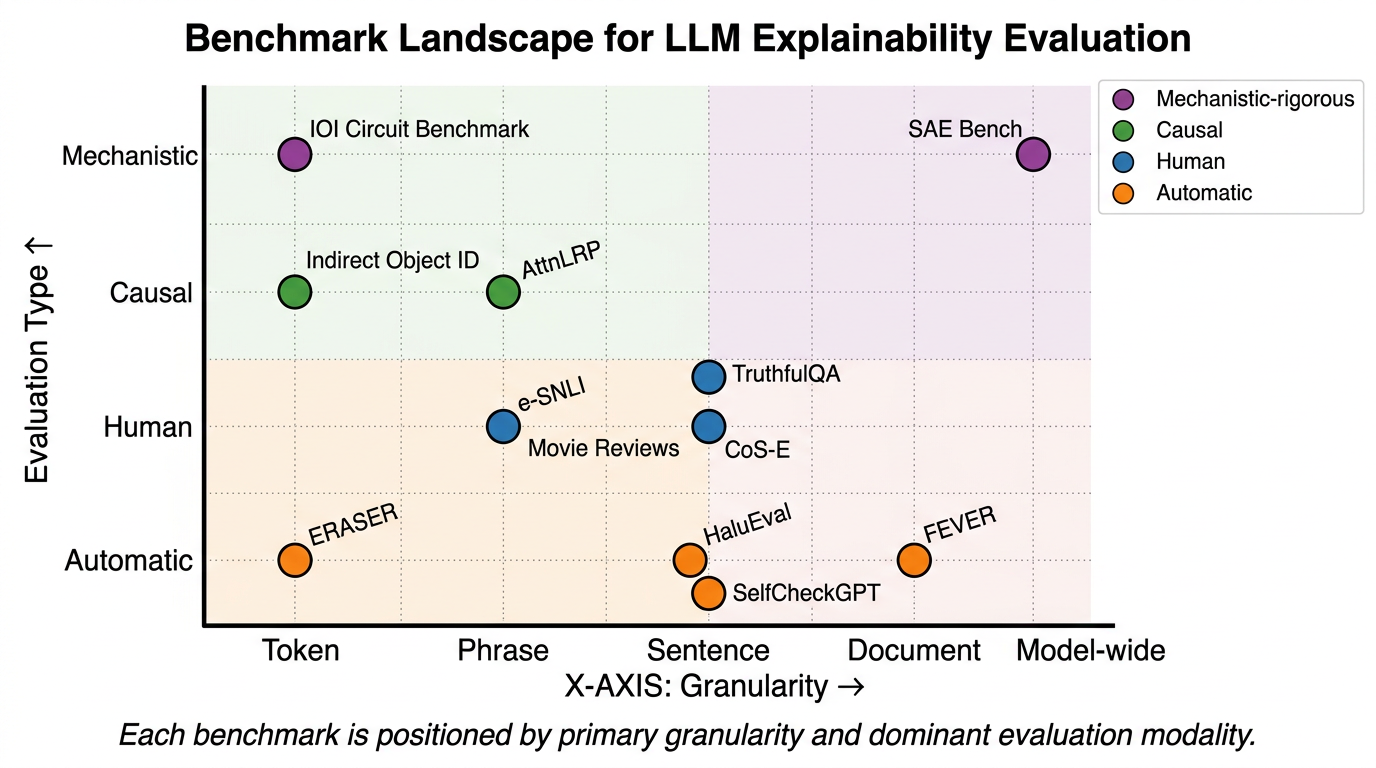
\includegraphics[width=\linewidth,keepaspectratio]{./figures/Explainability-for-Large-Language-Models__fig_benchmarks.png}}
\caption{Benchmark landscape for LLM explainability evaluation, plotted on granularity × evaluation-type axes.}\label{fig:fig-benchmarks}\end{figure}

\subsection{Explanation-generation datasets}\label{explanation-generation-datasets}

\emph{e-SNLI} (Camburu et al., 2018 NeurIPS) extends the 570K-example SNLI corpus with crowdsourced free-text explanations for each (premise, hypothesis, label) triple. Annotators wrote explanations averaging 14.5 tokens; inter-annotator BLEU is \textasciitilde25, providing a ceiling for automatic metrics. \emph{CoS-E} (Rajani et al., 2019 ACL) provides 10,962 commonsense-QA examples with explanations, designed to support training rationale-generation models. \emph{FLUTE} (Chakrabarty et al., 2022 EMNLP) provides 9,000 figurative-language NLI examples with explanations focusing on metaphor and sarcasm. \emph{e-ViL} \citep{kayser2021eviladatasetandben} is the multimodal counterpart with VQA-X (32K), e-SNLI-VE (4M visual NLI pairs), and VCR (290K commonsense visual reasoning).

\emph{ERASER} (DeYoung et al., 2020 ACL) is the principal multi-task benchmark for extractive rationales. It unifies seven datasets --- BoolQ (16K), MovieReviews (2K), MultiRC (32K), FEVER (185K), Evidence Inference (10K), CoS-E (10K), e-SNLI (570K) --- under a common annotation schema where each example has highlighted token spans serving as the rationale. ERASER introduced the \emph{comprehensiveness} and \emph{sufficiency} metrics that remain the standard for extractive faithfulness.

\emph{ScienceQA} (Lu et al., 2022 NeurIPS) provides 21,208 multiple-choice science questions with chain-of-thought rationales, useful for educational explanation evaluation. \emph{StrategyQA} (Geva et al., 2021) provides 2,780 implicit-reasoning questions with decomposition explanations. \emph{DROP} (Dua et al., 2019) provides 96K paragraph-comprehension questions where the answer requires discrete operations and the chain-of-thought is testable.

\subsection{Mechanistic test-beds}\label{mechanistic-test-beds}

\emph{TracrBench} \citep{thurnherr2024tracrbenchgenerati} compiles 12 hand-written programs (sorting, copying, reversing) into Tracr models with known ground-truth circuits, providing a faithfulness ceiling for automated discovery; current best F1 averages 0.79 across the suite. \emph{Othello-GPT} \citep{li2024pmetprecisemodeled} is a 1.5M-game corpus on which a small transformer is trained to predict legal moves; linear probes recover the board-state from middle-layer activations with F1 \textasciitilde0.96, establishing the model has \emph{learned} a board representation. \emph{RAVEL} \citep{huang2023asurveyonhallucina} tests representation-attribution: each input has multiple attributes (e.g., a city has country, population, language) and the benchmark scores whether intervention methods can isolate one attribute without affecting others. \emph{IOI prompt set} \citep{wang2022interpretabilityin} is a 1,000-prompt evaluation suite for the Indirect Object Identification circuit. \emph{Greater-Than circuit} (Hanna et al., 2023) provides a 1,000-prompt evaluation for numeric comparison. \emph{Docstring} (Heimersheim \& Nanda) provides synthetic Python docstring completion tasks with localised circuits.

These mechanistic test-beds matter because they give the field a \emph{ground truth}: a known circuit against which automated discovery can be evaluated. Without them, claims of mechanistic understanding are unfalsifiable.

\subsection{Hallucination and faithfulness benchmarks}\label{hallucination-and-faithfulness-benchmarks}

\emph{TruthfulQA} (Lin et al., 2022 ACL) --- 817 questions across 38 categories. \emph{HalluDial} \citep{luo2024localinterpretatio} --- 4,094 dialogues, sentence-level annotations. \emph{DiaHalu} \citep{chen2024diahaluadialoguele} --- multi-turn conversational hallucination. \emph{HaluEval} (Li et al., 2023 EMNLP) --- 35K samples spanning QA, dialogue, and summarisation with synthesised and human-annotated hallucinations. \emph{FELM} \citep{chen2024diahaluadialoguele} --- fine-grained factuality evaluation. \emph{Poly-FEVER} \citep{zhang2025jailbreakdistillat} --- multilingual fact verification across 11 languages. \emph{MedQA} (used by Med-PaLM, Singhal et al., 2023) --- USMLE-style medical QA (12,723 questions). These benchmarks support both \emph{detection} metrics (AUROC) and \emph{mitigation} metrics (factuality after intervention).

\subsection{Editing benchmarks}\label{editing-benchmarks}

\emph{ZsRE} (Levy et al., 2017) --- 240K zero-shot relation-extraction queries used by ROME for single-fact editing. \emph{CounterFact} (Meng et al., 2022) --- 21,919 counterfactual statements paired with paraphrases for generalisation testing. \emph{MQuAKE} (Zhong et al., 2023 EMNLP) --- 9,218 multi-hop edit queries across 1,800 base edits. \emph{RippleEdits} (Cohen et al., 2024 TACL) --- 5,000 edits with six categories of dependent fact (Logical Generalisation, Compositionality I/II, Subject Aliasing, Relation Specificity, Forgetfulness). \emph{KnowEdit} \citep{zhang2024acomprehensivestud} --- unified suite covering insertion, modification, deletion, erasure with reliability/generalisation/locality/portability metrics.

\subsection{Faithfulness, simulatability, and L0/loss-recovered metrics}\label{faithfulness-simulatability-and-l0loss-recovered-metrics}

The metric vocabulary of LLM explainability is dense. We summarise the principal entries.

\begin{table*}[t]
\centering
\caption{Faithfulness, simulatability, and L0/loss-recovered metrics: comparative summary.}
\label{tab:faithfulness-simulatability-and-l0-loss-recovered-metrics}
\begin{tabular}{>{\raggedright\arraybackslash}p{0.2718\linewidth}
  >{\raggedright\arraybackslash}p{0.0971\linewidth}
  >{\raggedright\arraybackslash}p{0.4369\linewidth}
  >{\raggedright\arraybackslash}p{0.1942\linewidth}}
\toprule
Metric & Family & Definition & Higher is better \\
\midrule
Comprehensiveness (Comp) & Extractive & Δ confidence when rationale removed & Yes \\
Sufficiency (Suff) & Extractive & Confidence with rationale only & Yes \\
Simulatability & Free-text & Sim. accuracy given rationale & Yes \\
Leakage-Adj. Sim. & Free-text & Sim. minus label-leakage baseline & Yes \\
BLEU / METEOR / BERTScore & Free-text & Lexical/semantic similarity to gold & Yes \\
Fidelity & Post-hoc & Surrogate vs.~model agreement & Yes \\
Sensitivity-N & Saliency & Spearman ρ between scores and N-removed Δ & Yes \\
Sufficiency-N (deletion AUC) & Saliency & AUC of confidence vs.~tokens removed & Yes \\
Reconstruction MSE & SAE & ‖x − x̂‖² & No \\
L0 sparsity & SAE & mean active features per token & No (lower better) \\
Loss-recovered fraction & SAE & 1 − (L\_with\_SAE − L\_clean)/(L\_zero − L\_clean) & Yes \\
Feature interpretability & SAE & \% features judged monosemantic by labeller & Yes \\
KL on patched logits & Mech. & KL(M\_patched ‖ M\_clean) & No (lower better) \\
Circuit F1 & Mech. & F1 of recovered components vs.~ground truth & Yes \\
AUROC (hallucination) & Black-box & ROC AUC on hallucinated vs.~faithful & Yes \\
Reliability (editing) & Editing & Edit applied correctly & Yes \\
Generalisation (editing) & Editing & Paraphrase consistency post-edit & Yes \\
Locality (editing) & Editing & Unrelated facts unchanged & Yes \\
Portability (editing) & Editing & Dependent facts updated & Yes \\
Early-truncation gap & CoT & Δ accuracy with partial CoT & Depends on direction \\
Paraphrase invariance & CoT & Answer consistency under CoT paraphrase & Yes \\
Unlearning faithfulness & CoT & Δ answer after step-specific unlearning & Yes (if positive) \\
\end{tabular}
\end{table*}

Modern papers typically report 3--5 of these metrics, reflecting the fact that no single metric captures all aspects of explanation quality.

\subsection{Cross-benchmark relationships}\label{cross-benchmark-relationships}

A growing meta-evaluation literature studies how benchmark choices interact. Bodria et al.~(2023, DMKD) found that LIME and KernelSHAP have Spearman ρ = 0.72 on ordinary inputs but only 0.41 on adversarially perturbed ones, demonstrating that benchmark stability matters. Atanasova et al.~(2020) showed that the comprehensiveness metric ranks methods differently than human-rated faithfulness, suggesting either comprehensiveness or human ratings is mis-specified. The \emph{Feature Attribution Stability Suite} \citep{subramaniakuppusamy2026featureattribution} is the most recent attempt to provide a unified stability evaluation across attribution methods.

\subsection{Reproducibility infrastructure}\label{reproducibility-infrastructure}

A non-trivial obstacle to evaluation is reproducibility. Three open-source frameworks dominate. \emph{TransformerLens} \citep{nanda2023progressmeasuresfo} provides hookable HuggingFace transformer implementations for GPT-2, GPT-J, Pythia, Llama, Mistral, and Gemma; the standard tool for activation patching, ACDC, and probing. \emph{nnsight} (Fiotto-Kaufman et al., 2024) supports any HuggingFace model with a uniform tracing API. \emph{Pyvene} \citep{wu2024fromlanguagemodeli} provides composable interventions. \emph{SAELens} (Bloom et al., 2024) is the standard SAE training and evaluation library. \emph{Neuronpedia} hosts \textgreater130M extracted SAE features as a browseable web service. \emph{EasyEdit} \citep{wang2023scottselfconsisten} is a unified editing toolkit; \emph{Inseq} (Sarti et al., 2023) standardises feature-attribution interfaces; \emph{captum} (Kokhlikyan et al., 2020) provides PyTorch-native attribution.

\subsection{Reported benchmark scores (representative)}\label{reported-benchmark-scores-representative}

\begin{table*}[t]
\centering
\caption{Reported benchmark scores (representative): comparative summary.}
\label{tab:reported-benchmark-scores-representative}
\begin{tabular}{>{\raggedright\arraybackslash}p{0.2553\linewidth}
  >{\raggedright\arraybackslash}p{0.3191\linewidth}
  >{\raggedright\arraybackslash}p{0.1596\linewidth}
  >{\raggedright\arraybackslash}p{0.2660\linewidth}}
\toprule
Method & Benchmark & Score & Citation \\
\midrule
Standard prompting & GSM8K (PaLM 540B) & 17.9\% & Wei et al.~2022 \\
CoT prompting & GSM8K (PaLM 540B) & 56.5\% & Wei et al.~2022 \\
CoT + Self-Consistency & GSM8K (PaLM 540B) & 74.4\% & Wang et al.~2023 \\
Faithful CoT (Python) & GSM8K & 95.0\% & Lyu et al.~2023 \\
ACDC & IOI (GPT-2 small) & F1 0.85 & Conmy et al.~2023 \\
EAP & IOI (GPT-2 small) & F1 0.91 & Syed et al.~2024 \\
ROME & CounterFact GPT-2 XL & 91\% reliability & Meng et al.~2022 \\
MEMIT & CounterFact 10K edits GPT-J 6B & 89\% reliability & Meng et al.~2023 \\
MEMIT & MQuAKE-CF 2-hop GPT-J 6B & 21\% & Zhong et al.~2023 \\
In-Context & MQuAKE-CF GPT-3.5 & 72\% portability & Cohen et al.~2024 \\
Med-PaLM & MedQA (USMLE) & 67.6\% & Singhal et al.~2023 \\
Token entropy & TriviaQA AUROC & 0.78 & Farquhar et al.~2024 \\
Semantic entropy & TriviaQA AUROC & 0.85 & Farquhar et al.~2024 \\
SelfCheckGPT-NLI & GPT-3 facts AUROC & 0.83 & Manakul et al.~2023 \\
34M-feature SAE & Claude 3 Sonnet loss-rec & 0.92 & Templeton et al.~2024 \\
Gated SAE & Pythia-2.8B loss-rec & 0.94 & Rajamanoharan et al.~2024 \\
TopK SAE & GPT-4 family loss-rec & 0.965 & Gao et al.~2024 \\
TracrBench avg F1 (auto) & TracrBench & 0.79 & Thurnherr \& Scheurer 2024 \\
Othello-GPT linear probe & Board state F1 & 0.96 & Li et al.~2023 \\
\end{tabular}
\end{table*}

\subsection{The benchmark gap}\label{the-benchmark-gap}

Despite this density of resources, two systematic gaps persist. First, there is no widely adopted \emph{unified faithfulness leaderboard} --- papers report different metric subsets on different splits. Second, \emph{frontier-model} benchmarks remain undeveloped: most explainability benchmarks target GPT-2-scale models because their behaviour is testable in a small lab; the explainability of GPT-4o, Claude 3 Opus, and Gemini 1.5 Pro is evaluated only piecemeal. Sharkey et al.~(2025) flag the development of frontier-scale faithfulness benchmarks as an urgent open problem; the \emph{Open Problems in Mechanistic Interpretability} paper specifically calls for benchmarks that test SAE features for causal sufficiency rather than reconstruction quality alone.

A further concern is the \emph{test-set contamination} problem: as models train on increasingly large fractions of the public internet, public benchmarks may leak into pretraining data. TruthfulQA, GSM8K, and MMLU all show partial contamination in modern frontier models, complicating the interpretation of reported scores. The community has begun to use \emph{held-out} and \emph{temporally novel} test sets --- questions written after a model's training cutoff --- to mitigate contamination. \emph{Jailbreak Distillation} \citep{zhang2025jailbreakdistillat} proposes ``renewable safety benchmarking'' via continual distillation of new test cases.

\subsection{What an ideal benchmark would look like}\label{what-an-ideal-benchmark-would-look-like}

For LLM explainability to mature as a measurable engineering discipline, we believe four properties are essential. (1) \emph{Causal faithfulness}: a metric that fails when an explanation is correlational; semantic entropy and the unlearning-based CoT metric are early instances. (2) \emph{Frontier-model coverage}: tests that scale to 70B+ models without prohibitive compute, e.g., attribution patching at scale. (3) \emph{Domain transfer}: explanations evaluated for both general and domain-specific (medical, legal) tasks. (4) \emph{Reproducibility infrastructure}: code, weights, and evaluation harness released together. The \emph{KnowEdit} and \emph{RippleEdits} benchmarks for editing meet criteria (1) and (4); \emph{Gemma Scope} and \emph{Llama Scope} enable (2). The integration of these into a single unified suite is the obvious next step, and we expect 2026--2028 to deliver it.

\section{Applications: Healthcare, Safety, Multilingual and Multimodal Settings}\label{applications-healthcare-safety-multilingual-and-multimodal-settings}

Whereas Section~9 catalogued evaluation infrastructure, this section turns to deployment domains where LLM explainability has measurable impact. The biomedical strand is anchored by Med-PaLM 2 \citep{singhal2023largelanguagemodel} at 67.6\% on MedQA, alongside BioGPT (Luo et al., 2022) as a biomedical backbone, PubMedBERT (Gu et al., 2021) as a biomedical encoder, and MedAlpaca (Han et al., 2023) as an instruction-tuned medical LLM. The multimodal frontier comprises LLaVA (Liu et al., 2023) as a vision-language assistant, Qwen-VL (Bai et al., 2023) as the multimodal Qwen, GPT-4V (OpenAI, 2023) as a vision-language frontier model, Gemini 1.5 Pro (Google, 2024) as a multimodal long-context system, and Whisper (Radford et al., 2023) for audio. Prisma \citep{joseph2025prismaanopensource} provides a multimodal SAE toolkit. Safety-oriented deployments include Refusal Direction Editing (Arditi et al., 2024) for jailbreaks via residual ablation, the PIEE Cycle \citep{trabilsy2025thepieecycleastruc} for clinical red-teaming, and MTSA \citep{guo2025mtsamultiturnsafet} for multi-turn safety alignment. The reasoning frontier is occupied by DeepSeek-R1 (DeepSeek-AI, 2025), an RL-trained reasoning model.

LLM explainability is no longer purely an academic exercise. Healthcare deployments demand auditable rationales, AI-safety teams use mechanistic methods to understand jailbreak vulnerabilities, and multilingual and multimodal extensions test cross-setting transfer of techniques developed for English text-only LLMs.

\subsection{Clinical decision support and biomedical LLMs}\label{clinical-decision-support-and-biomedical-llms}

Medical LLMs are the canonical high-stakes application. \emph{Med-PaLM 2} (Singhal et al., 2023 Nature) achieves 67.6\% accuracy on the USMLE-style MedQA benchmark and uses CoT rationales validated by clinician panels. The validation protocol --- clinician scoring on six axes (alignment with consensus, no relevant information missing, no incorrect content, no harm, no bias, comprehension of intent) --- is essentially a plausibility-and-faithfulness audit. \emph{BioGPT} (Luo et al., 2022) and \emph{PubMedBERT} (Gu et al., 2021) provide biomedical-domain backbones; \emph{AlphaMed} and \emph{MedAlpaca} are instruction-tuned variants. The principal explainability tool deployed in clinical workflow is retrieval-augmented chain-of-thought, where each medical claim in the rationale is grounded to a specific document.

Recent clinical applications include: \emph{Triage prediction} (Lee et al., 2026 JAMIA) used BERT-based classifiers on emergency-department conversations with SHAP attributions. \emph{ICU decision support} (Lee et al., 2025 BMC) uses SHAP for feature importance combined with LLM-generated explanations. \emph{Visual prognosis prediction} in age-related macular degeneration (Zhao et al., 2027 Lancet Digital Health) couples deep learning with explainability. \emph{Quality-of-care measurement for ADHD} (Bannett et al., 2026 medRxiv) evaluates LLMs for transparent care metrics. \emph{Cancer germline testing pathway} (Mason et al., 2026 NCCN) deploys LLM-based decision support with explanation traces.

The PIEE Cycle \citep{trabilsy2025thepieecycleastruc} provides a structured red-teaming framework for clinical LLMs: Probe, Identify, Evaluate, Escalate. The cycle integrates black-box auditing (semantic entropy, SelfCheckGPT) with domain-expert review. \emph{Readability} concerns matter: Maywald et al.~(2025 Current Oncology) showed that 12\% of adults have proficient health literacy, demanding plain-language explanations alongside technical rationales.

\subsection{AI safety, jailbreak analysis, and steering vectors}\label{ai-safety-jailbreak-analysis-and-steering-vectors}

Mechanistic interpretability is increasingly applied to AI safety. The 2024 Anthropic \emph{Scaling Monosemanticity} report identified SAE features for \emph{deception}, \emph{secret keeping}, and \emph{sycophancy} in Claude 3 Sonnet, showing they activate in safety-relevant contexts. Clamping the \emph{refusal} feature reduces refusal rate; clamping the \emph{sycophancy} feature decreases user-pleasing tendencies.

Jailbreak research is a cousin of explainability. \emph{GPTFUZZER} \citep{yu2023gptfuzzerredteamin} auto-generates jailbreak prompts; \emph{Sirens' Whisper} (Gao et al., 2023) demonstrates near-ultrasonic jailbreaks of speech LLMs; \emph{MTSA} (Guo et al., 2025 ACL) extends safety alignment to multi-turn dialogues. The defence side: Wei et al.~(2026 IEEE TPAMI) propose few-in-context demonstrations that guard aligned LLMs against jailbreaks. \emph{Latent Adversarial Training} \citep{sheshadri2024latentadversarialt} improves robustness to persistent harmful behaviours. \emph{BlueSuffix} \citep{zhao2024explainabilityforl} defends vision-language models against jailbreaks. \emph{LLM Stinger} (Jha et al., 2025 AAAI) and \emph{TombRaider} (Ding et al., 2025 EMNLP) extend the attack surface; \emph{SearchAttack} (Yan et al., 2026) uses online web search as a jailbreak vector.

The mechanistic-interpretability approach to safety is best illustrated by Arditi et al.'s (2024) \emph{refusal-direction} analysis: a single residual-stream direction in Llama-2-7B-Chat mediates \textasciitilde80\% of refusal behaviour, and ablating it produces a model that complies with harmful queries. Conversely, \emph{one-shot optimised steering vectors} \citep{dunefsky2025oneshotoptimizedst} can mediate safety-relevant behaviours with minimal data. \emph{Honesty steering} (Góral et al., 2025) targets the gap between models' internal beliefs and stated answers.

\subsection{Multilingual probing and explainability}\label{multilingual-probing-and-explainability}

The multilingual extension of LLM explainability is mapped by Resck, Augenstein and Korhonen (2025 EMNLP), surveying ≥80 studies. Key findings: (i) probing recovers similar syntactic information across high-resource languages but is much weaker on low-resource ones; (ii) \emph{concept directions} are largely language-agnostic in the late layers \citep{dumas2024separatingtonguefr}, validating the \emph{language-thought separation} hypothesis (Mahowald et al., 2024 TICS); (iii) edits in English do not transfer to other languages without retraining. \emph{Multilingual probing of contextual encoders} \citep{ravishankar2019multilingualprobin} was the early benchmark for this work; current evaluation uses XCOPA, XGLUE, MASSIVE, and the Belebele reading-comprehension benchmark across 100+ languages. Zhang et al.~(2025 Cybersecurity) survey multilingual safety in cybersecurity. \emph{Chinese classifier prediction} \citep{zhang2025jailbreakdistillat} compares BERT and modern LLMs on a language-specific phenomenon. \emph{Function induction} \citep{ye2025functioninductiona} and \emph{separating tongue from thought} \citep{dumas2024separatingtonguefr} provide deeper mechanistic claims.

\subsection{Multimodal LLMs (MLLMs)}\label{multimodal-llms-mllms}

Multimodal LLMs combine language with vision (LLaVA, Qwen-VL, GPT-4V, Gemini 1.5 Pro), audio (Whisper, Qwen-Audio), or video (Video-LLaMA). Dang et al.~(2024) survey explainability for MLLMs comprehensively; Ghosh et al.~(2024) survey vision-language models. Key methods transferred from text: \emph{LIME-Vision} and \emph{SHAP-Vision} for token attribution; CoT rationales adapted to grounded reasoning (Visual Chain-of-Thought); SAEs trained on multimodal residual streams (Joseph et al., 2025 Prisma toolkit). \emph{Mechanistic interpretability of Vision Transformers} \citep{bahador2025mechanisticinterpr} and \emph{Seeing Through Circuits} (Żukowska et al., 2026) extend circuit-level analysis to ViT. \emph{e-ViL} \citep{kayser2021eviladatasetandben} is the principal benchmark with VQA-X (32K), e-SNLI-VE, and VCR (290K). \emph{Dr.~SHAP-AV} (Cappellazzo et al., 2026) adapts SHAP to audio-visual speech recognition.

The challenges differ from text: ViT and CLIP-style encoders sit upstream of the language model, so explanations must trace causality across modality boundaries. Interpretable medical VQA \citep{hu2024understandingreaso} uses multimodal relationship graphs to provide attribution. The 2024--2026 frontier is \emph{cross-modal feature linking}: which SAE features in the language stream correspond to which patches in the visual stream?

\subsection{Education and tutoring}\label{education-and-tutoring}

Educational deployments of LLMs require explainability for both teacher review and student comprehension. Kasneci et al.~(2023 Learning and Individual Differences) surveyed ChatGPT-in-education; explainability is identified as a top research priority. Worked examples generated by LLMs (with stepwise CoT rationales) provide both pedagogical content and a faithfulness anchor --- students can evaluate whether the steps make sense. \emph{MultiSense-L2Net} (Abbas et al., 2026) uses AI-mediated co-regulation in second-language writing. \emph{Cognitive Flow} (Dissanayake \& Nanayakkara, 2025) studies AI interventions for reasoning support. The principal interpretability tools deployed in education are CoT rationales and retrieval grounding, both of which are robust to closed-API constraints.

\subsection{Finance, law, and other regulated domains}\label{finance-law-and-other-regulated-domains}

Financial-services applications of LLM interpretability are surveyed by Golgoon et al.~(2024 ICAIF), who specifically examine activation patching and probing on financial-text models. Cybersecurity applications are surveyed by Zhang et al.~(2025 Cybersecurity). Legal applications are nascent --- Casetext's CoCounsel and LexisNexis Lexis+ AI are commercial deployments --- and lean heavily on retrieval-augmented faithfulness anchors. The EU AI Act (2024) classifies LLM-based legal advice as a high-risk system, requiring traceability documentation that mechanistic interpretability tools could in principle supply.

\subsection{Reinforcement-learning aligned LLMs}\label{reinforcement-learning-aligned-llms}

LLMs aligned with RLHF or RLAIF acquire new behaviours that demand fresh interpretation. Liu et al.~(2025) survey RL-meets-LLM. \emph{Reasoning-tuned} models such as OpenAI o1 and DeepSeek-R1 (DeepSeek-AI, 2025) produce long CoT chains whose faithfulness has not yet been characterised. \emph{Improving Reasoning via Representation Engineering} (Højer et al., 2025) shows that reasoning behaviour can be elicited via steering vectors, suggesting reasoning is mediated by specific residual-stream directions amenable to interpretation.

\subsection{Application-domain summary}\label{application-domain-summary}

\begin{table*}[t]
\centering
\caption{Application-domain summary: comparative summary.}
\label{tab:application-domain-summary}
\begin{tabular}{>{\raggedright\arraybackslash}p{0.1250\linewidth}
  >{\raggedright\arraybackslash}p{0.2212\linewidth}
  >{\raggedright\arraybackslash}p{0.2885\linewidth}
  >{\raggedright\arraybackslash}p{0.1827\linewidth}
  >{\raggedright\arraybackslash}p{0.1827\linewidth}}
\toprule
Domain & Primary task & Dominant explainability method & Key benchmark & Citation \\
\midrule
Medicine & QA / triage & CoT + RAG + clinician audit & MedQA (12.7K) & Singhal et al.~2023 \\
ICU support & Risk stratification & SHAP + LLM rationale & MIMIC-III/IV & Lee et al.~2025 \\
Safety & Jailbreak defence & Refusal direction, steering & HarmBench, AdvBench & Arditi et al.~2024 \\
Multilingual & Cross-lingual NLI & Probing + activation patching & XGLUE, Belebele & Dumas et al.~2024 \\
Multimodal & VQA + rationale & SHAP-V + CoT & VQA-X (32K), e-ViL & Kayser et al.~2021 \\
Education & Tutoring & CoT + retrieval grounding & ScienceQA (21K) & Lu et al.~2022 \\
Finance & Risk / fraud & Probing + patching & Domain-specific & Golgoon et al.~2024 \\
Cybersecurity & Vulnerability detection & LLM CoT + verification & DeepSeek-R1 eval & Zhang et al.~2025 \\
Legal & Case retrieval & Retrieval + citation grounding & LegalBench & (commercial) \\
Reasoning & Math / code & CoT + Faithful CoT & GSM8K, MATH & Wei et al.~2022 \\
\end{tabular}
\end{table*}

\subsection{Cross-domain lessons}\label{cross-domain-lessons}

Three cross-domain lessons emerge. First, \emph{RAG anchors} are a remarkably consistent pattern: when a domain demands faithful explanations, retrieval-augmented citation provides a ground-truth check that pure CoT lacks. Second, \emph{human review} remains the gold standard, with interpretability tools serving to make that review tractable rather than to replace it. Third, \emph{domain-specific benchmarks} substantially outperform general ones: a hallucination detector trained on TriviaQA does not transfer well to MedQA. The deployment success of Med-PaLM and the slow progress of legal LLMs reflect this gap.

\subsection{Outlook for application-driven explainability}\label{outlook-for-application-driven-explainability}

Three trends are reshaping deployment. First, \emph{regulation-driven evaluation}: the EU AI Act requires traceability for high-risk systems, pushing interpretability from research into compliance. Second, \emph{agentic LLMs}: tool-using agents \citep{wang2023scottselfconsisten} demand explanations of multi-step decisions, blurring the line between CoT, retrieval, and tool-call traces; the \emph{AIOps} survey \citep{zhang2025jailbreakdistillat} maps this for IT operations. Third, \emph{cross-modal}: as medical and scientific deployments combine text with images and structured data, explanations must trace causality across modality boundaries, with \emph{Dr.~SHAP-AV} and Prisma \citep{joseph2025prismaanopensource} as early instances. Clinical and legal deployment will be the principal forcing function for explainability research over the next five years, much as ImageNet shaped computer vision in the 2010s.

\section{Limitations, Failure Modes, and Adversarial Threats to Explanations}\label{limitations-failure-modes-and-adversarial-threats-to-explanations}

Whereas Section~10 surveyed application successes, this section catalogues failure modes and adversarial threats. The adversarial-attribution strand opens with Fooling LIME and SHAP \citep{slack2020foolinglimeandshap}, a 95\% scaffold-detection attack, and the SHLIME defence \citep{chauhan2025shlimefoilingadver} as the anti-scaffold technique. Explanation Bias \citep{kamp2025explanationbiasisa} further exposes lexical and positional bias in Integrated Gradients. Chain-of-Thought failures cluster around four results: the biasing-feature CoT shift of Turpin et al.~(2023), with 36\% silent answer change; the paraphrase non-invariance of Lanham et al.~(2023), where surface form drives CoT; the unlearning-based finding of Tutek et al.~(2025) that fewer than 40\% of CoT steps are causally necessary; and CoT in the Wild \citep{arcuschin2025chainofthoughtreas}, which characterises naturally occurring chains as post-hoc rationalisation. Editing failures include the specificity collapse of Hoelscher-Obermaier et al.~(2023) with 15--25\% silent corruption, and the multi-hop ripple failure of Zhong et al.~(2023) where 2-hop accuracy falls to 21\%. SAE-side limits include Circular Features \citep{engels2024notalllanguagemode} for non-linear feature manifolds and the reconstruction-behaviour gap of Braun et al.~(2024) between MSE and KL divergence. The COVID Shortcut paper \citep{degrave2021aiforradiographicc} remains the canonical saliency-shortcut cautionary tale.

Explanations can fail in several systematic ways: they can be unfaithful (correlate poorly with model causation), brittle (sensitive to input perturbations), gameable (manipulable by an adversary), or \emph{correct but useless} (technically faithful but cognitively unintelligible). The remainder of this section reports specific empirical demonstrations of each failure regime, building a conservative picture of what current LLM explainability cannot yet do.

\subsection{Fooling LIME and SHAP: adversarial saliency}\label{fooling-lime-and-shap-adversarial-saliency}

Slack et al.~(2020 AIES) showed that an adversary controlling the model can produce LIME and SHAP explanations that hide a biased decision rule. The construction inserts a \emph{scaffold} classifier. The scaffold detects perturbed inputs (used by LIME) versus original inputs and routes them to different sub-models. A fair sub-model handles perturbations and generates the explanation. A biased sub-model handles actual queries. The technique fools both LIME and KernelSHAP across the COMPAS, Communities and Crime, and German Credit datasets, with scaffold-detection accuracy \textgreater95\%. The impact is that LIME and SHAP explanations cannot be trusted in adversarial settings without auxiliary integrity checks. \emph{SHLIME} \citep{chauhan2025shlimefoilingadver} and the \emph{Feature Attribution Stability Suite} \citep{subramaniakuppusamy2026featureattribution} develop defences but do not eliminate the threat. The methodological lesson is that local post-hoc methods that perturb the input must verify the model behaves consistently inside and outside the perturbation distribution.

A related result is \emph{Explanation Bias} \citep{kamp2025explanationbiasisa}: post-hoc feature attributions exhibit lexical and positional biases independent of the underlying decision, because Integrated Gradients and similar methods over-attribute to the first token and to high-frequency words. \emph{Forward-Learning Saliency} \citep{zhang2024acomprehensivestud} attempts black-box-compatible saliency without gradient access but inherits the same biases.

\subsection{Unfaithful Chain-of-Thought}\label{unfaithful-chain-of-thought}

Section 6 documented the principal CoT-faithfulness failures. We summarise the most important: (i) \emph{Biasing-feature unfaithfulness} \citep{turpin2023languagemodelsdont}: when GPT-4 is given a prompt with a biasing pattern (e.g., always answer ``(A)''), the model often switches its answer without acknowledging the bias in the rationale; on BBH, 36\% of answers shift silently. (ii) \emph{Paraphrase non-invariance} \citep{lanham2023measuringfaithfuln}: paraphrasing a CoT chain changes the answer with non-trivial frequency, indicating the surface form rather than the logical content drove the prediction. (iii) \emph{Unlearning faithfulness} \citep{tutek2025measuringchainofth}: on Llama-3-8B GSM8K, fewer than 40\% of CoT steps are causally necessary; 22\% of answers can be predicted from the model's representations \emph{before} the CoT begins. (iv) \emph{Reasoning in the wild} \citep{arcuschin2025chainofthoughtreas}: even without explicit biasing, naturally occurring CoT chains are post-hoc rationalisations roughly 25--30\% of the time.

The implication is that CoT-as-explanation requires audit. A clinical or legal deployment that relies on the rationale must either pair it with retrieval grounding (so that each claim cites a verifiable source) or with a faithfulness probe (so that internal-state evidence corroborates the rationale).

\subsection{The brittleness of probes}\label{the-brittleness-of-probes}

Hewitt and Liang's (2019) control-task warning remains relevant. A probe that recovers a property may be exploiting its own expressivity rather than the underlying model's representation. The \emph{selectivity} metric (task minus control accuracy) is a partial fix but does not resolve the deeper issue: a high-selectivity probe still cannot distinguish between a property genuinely encoded by the model and a property reconstructible from incidental features. Shin et al.~(2020 EMNLP) showed that AutoPrompt-discovered probes can elicit knowledge from BERT that supervised probes cannot, suggesting that probes are biased estimators of what a model ``knows''.

A second probe pathology is \emph{cross-task transfer failure}: a probe trained to recover X from layer ℓ does not transfer to a task that relies on X downstream, indicating the probe captures a \emph{probe-readable} version of X that may not be what the model uses. Hase et al.~(2023) showed this for factual recall: causal-tracing-localised facts do not transfer to editing accuracy.

\subsection{Superposition and the limits of SAE features}\label{superposition-and-the-limits-of-sae-features}

SAEs assume an \emph{additive} feature decomposition: x ≈ Σ\emph{i \(z_i\) · \(d_i\) where \(d_i\) are dictionary elements. Several pathologies undermine this assumption. (i) \_Multi-dimensional features} \citep{engels2024notalllanguagemode}: some features are encoded on circular manifolds (days-of-week, months) that linear dictionaries cannot capture without redundancy. (ii) \emph{Cross-layer mixing} (Lindsey et al., 2024): features at later layers are non-trivially compositions of features at earlier layers; per-layer SAEs miss this. (iii) \emph{Feature splitting at higher m}: increasing dictionary width causes features to fragment into non-orthogonal sub-features. (iv) \emph{Reconstruction--behavior gap} \citep{braun2024identifyingfunctio}: low MSE does not imply preserved downstream behaviour. (v) \emph{Adversarial vulnerability} \citep{bereska2024mechanisticinterpr}: high superposition correlates with adversarial brittleness, suggesting SAEs are diagnosing rather than eliminating a fundamental representational risk.

\subsection{Editing failures}\label{editing-failures}

The editing literature has identified several reproducible failures. (i) \emph{Specificity collapse} under sequential edits --- after \textasciitilde5,000 sequential edits with MEMIT, GPT-J 6B begins corrupting unrelated facts. (ii) \emph{Multi-hop ripple failures} --- Zhong et al.~(2023) show that ROME/MEMIT edits propagate poorly to multi-hop queries (21\% accuracy at 2-hop). (iii) \emph{Cross-lingual transfer failures} --- edits in English do not propagate to Hindi or Chinese paraphrases \citep{wang2023scottselfconsisten}. (iv) \emph{Locality--portability conflict} --- methods that maximise locality fail at portability and vice versa. (v) \emph{Catastrophic forgetting in lifelong editing}. \emph{MEMIT-Merge} \citep{dong2025memitmergeaddressi} addresses same-subject batch-edit conflicts but not the broader specificity decay.

\subsection{Hallucination-detector failures}\label{hallucination-detector-failures}

Black-box hallucination detectors have characteristic failure modes. (i) Sample-consistency methods (SelfCheckGPT, semantic entropy) fail on \emph{consistently incorrect} hallucinations. The model is confidently wrong across all samples. Farquhar et al.~(2024) report this case explicitly. (ii) Detectors confuse \emph{aleatory} uncertainty (legitimate ambiguity) with \emph{epistemic} uncertainty (model error). (iii) RAG-based detectors fail when the retrieval system itself returns incorrect documents (28\% on noisy retrieval, Chen et al., 2024). (iv) Internal-state probes (CCS) suffer reliability degradation on out-of-distribution prompts. (v) Domain transfer is poor: a TriviaQA detector loses 8--15 AUROC points on MedQA without retraining.

\subsection{Computational and accessibility limits}\label{computational-and-accessibility-limits}

Many state-of-the-art interpretability methods are computationally heavy. ACDC at the IOI scale takes \textasciitilde3 GPU-hours; activation-patching sweeps on Llama-2 7B exceed 60 GPU-hours per task. Training a single SAE for Llama-3 8B costs hundreds of GPU-hours; the 34M-feature Claude SAE is reported (Templeton et al., 2024) to have consumed millions of dollars of compute. These costs put cutting-edge methods out of reach for most academic groups and concentrate progress in a few well-resourced industrial labs. Attribution patching \citep{syed2024attributionpatchin} and gated SAEs \citep{rajamanoharan2024improvingdictionar} are partial mitigations, but the asymmetry persists. Public releases such as Gemma Scope (Lieberum et al., 2024) help democratise access at the cost of fixing the hyperparameter choices made by the releasing team.

\subsection{Conceptual limits: the meaning of ``explanation''}\label{conceptual-limits-the-meaning-of-explanation}

A foundational concern, raised by Saphra and Wiegreffe (2024 BlackboxNLP) and Singh et al.~(2024 \emph{Rethinking Interpretability}), is that the term ``mechanistic'' can mislead: a circuit is \emph{one} causally sufficient implementation of a behaviour, not a uniquely correct one. Multi-realisability is unavoidable; circuit analysis can identify \emph{a} mechanism but not \emph{the} mechanism. This is not necessarily a bug --- for engineering purposes a sufficient mechanism is enough --- but it is a methodological constraint on how strongly mechanistic claims can be stated. Schneider's (2024) \emph{GenXAI} survey takes this further, arguing that explanations must be evaluated \emph{for whom} --- a regulator's needs differ from a user's, which differ again from a researcher's.

A related concern is \emph{cognitive accessibility}: a 26-head circuit graph for IOI is correct but largely unintelligible to a non-specialist. The end-user of a clinical decision-support system cannot read circuit diagrams; their explanation must be a natural-language summary, which reintroduces faithfulness questions. This is not a defect of mechanistic methods; it is a limit of the artifact. Explanations targeting different stakeholders use different artifacts, and the field has not solved the \emph{unifying explanation} problem.

\subsection{Failure-mode catalogue}\label{failure-mode-catalogue}

\begin{table*}[t]
\centering
\caption{Failure-mode catalogue: comparative summary.}
\label{tab:failure-mode-catalogue}
\begin{tabular}{>{\raggedright\arraybackslash}p{0.2500\linewidth}
  >{\raggedright\arraybackslash}p{0.1742\linewidth}
  >{\raggedright\arraybackslash}p{0.3106\linewidth}
  >{\raggedright\arraybackslash}p{0.2652\linewidth}}
\toprule
Failure mode & Method affected & Evidence & Mitigation \\
\midrule
Adversarial scaffold & LIME, SHAP & Slack et al.~2020: 95\% scaffold-detection & Integrity check on perturbations \\
Lexical/position bias & IG, GradCAM & Kamp et al.~2025 & De-biased gradients \\
Biasing-feature CoT & Chain-of-Thought & Turpin et al.~2023: 36\% silent shift & Pair with internal probe \\
Paraphrase shift & CoT & Lanham et al.~2023 & Self-consistency + invariance check \\
Unlearning unfaithfulness & CoT & Tutek et al.~2025: \textless40\% causal & Symbolic CoT, e.g., Faithful CoT \\
Probe expressivity & Linear probes & Hewitt \& Liang 2019 & Selectivity, control tasks \\
Circular features & SAE & Engels et al.~2024 & Multi-dim feature dictionaries \\
Reconstruction--behavior gap & SAE & Braun et al.~2024 & End-to-end SAE training \\
Specificity collapse & ROME/MEMIT & Hoelscher-Obermaier et al.~2023 & Better specificity benchmarks \\
Multi-hop ripple failure & ROME/MEMIT & Zhong et al.~2023: 21\% 2-hop & Multi-stage edits, In-Context \\
Confident hallucination & SelfCheckGPT & Farquhar et al.~2024 & Combine with retrieval \\
Domain transfer & Hallucination detectors & 8--15 AUROC drop & Domain-specific training \\
COVID shortcut & Saliency & DeGrave et al.~2021 & Causal probing, distribution shift \\
Localisation--editing dissociation & Causal tracing & Hase et al.~2023 & Editing-aware localisation \\
Cognitive inaccessibility & Circuits & n/a & Layered explanations by stakeholder \\
\end{tabular}
\end{table*}

\subsection{What ``honest about limits'' looks like}\label{what-honest-about-limits-looks-like}

Three rhetorical practices distinguish careful from overclaiming explainability work. First, report multiple metrics --- comprehensiveness, sufficiency, simulatability, causal influence --- because no single metric captures faithfulness. Second, report \emph{control} experiments: paraphrase invariance, biasing-feature consistency, perturbation robustness. Third, distinguish \emph{correlational} from \emph{causal} claims explicitly. Singh et al.~(2024) and Saphra and Wiegreffe (2024) provide model citations for this practice; the \emph{Rethinking Interpretability} paper specifically argues that the LLM era requires re-grounding interpretability on causal sufficiency rather than statistical correlation.

The COVID-19 chest-radiograph shortcut paper (DeGrave et al., 2021 Nature Machine Intelligence) is the canonical cautionary tale for the field: a model that achieves 99\% AUROC on COVID detection turns out to be using shortcuts (laterality markers, scan-bed style) rather than disease-relevant signal. Saliency methods such as Grad-CAM happily produced lung-localised heatmaps that masked the shortcut, because the saliency was correlated with the shortcut features that themselves correlated with the lung region. The paper is regularly invoked as the reason why explainability evaluation must include adversarial and out-of-distribution stress tests.

\subsection{Outlook}\label{outlook-2}

Limitations are an active research front, and mitigations are emerging: gated and end-to-end SAEs reduce reconstruction-behavior gap, symbolic and program-aided CoT recovers faithfulness in narrow domains, and editing-aware localisation begins to close the localisation-editing dissociation. The field, however, remains in a phase where every published method comes with a known failure regime. Researchers should \emph{report} known limitations on every method, and downstream users should treat any single-explanation deployment as a starting point that must be paired with audit.

\section{Open Problems and a Forecast for 2026--2030}\label{open-problems-and-a-forecast-for-20262030}

Building on the limitations in Section~11, this section delivers a structured catalogue of open problems and falsifiable forecasts for 2026--2030. The open problems are organised by methodological pillar --- SAE scaling, faithfulness benchmarks, faithful CoT, causal SAE evaluation, cross-layer linking, agentic interpretability, multimodal/multilingual, and regulation --- each paired with a measurable success criterion.

Our problem list inherits substantially from Sharkey et al.'s (2025 \emph{Open Problems in Mechanistic Interpretability}) but extends to the broader explainability scope of this survey, so that this section may be re-evaluated in 2030.

\subsection{Scaling SAEs and circuits to frontier models}\label{scaling-saes-and-circuits-to-frontier-models}

The single largest open problem is scaling. Mechanistic interpretability methods that work on GPT-2 small (117M, 12 layers) become prohibitive on Llama-3 70B (80 layers, 8192 hidden dim). Activation patching scales as O(L × H × T) where L is layers, H is heads per layer, T is tokens; an exhaustive sweep on Llama-3 70B for a 200-token prompt requires \textasciitilde10 million forward passes per prompt pair. Attribution patching \citep{syed2024attributionpatchin} reduces this to \textasciitilde10 backward passes but the linearisation breaks for non-linear circuits. SAEs at frontier scale require billions of parameters: Anthropic's 34M-feature SAE on Claude 3 Sonnet's residual stream consumed \textasciitilde2 × 10\^{}17 tokens of activations and on the order of \$1M of compute. Open problems include: (i) cheaper SAE variants (e.g., gated SAE at 16K width recovers most of the loss recovered by 1M-width vanilla SAE, Rajamanoharan et al., 2024); (ii) cross-model transfer (an SAE trained on Pythia-1.4B may not transfer to Pythia-12B); (iii) compositional SAEs that share a base across tasks.

\textbf{Forecast 1}: by 2027 a public SAE suite at 1M-feature width will be released for a 70B-parameter model with loss-recovered fraction ≥0.92. Falsified if no such suite exists by end-2027.

\subsection{Standardising faithfulness benchmarks}\label{standardising-faithfulness-benchmarks}

The field lacks a unified faithfulness leaderboard. Different papers report different metric subsets (comprehensiveness, sufficiency, simulatability, paraphrase invariance, unlearning faithfulness) on different splits. The closest candidate for a unified benchmark is the combination of ERASER (extractive), ChainPoll (CoT), and the unlearning protocol of Tutek et al.~(2025), but adoption remains uneven. A community-supported leaderboard is necessary for the field to track real progress vs.~method-specific tuning.

\textbf{Forecast 2}: by 2027 a community faithfulness leaderboard covering at least 5 method families (LIME/SHAP, ACDC, SAE-attribution, CoT-faithfulness, hallucination detection) will exist with regular submissions from at least 10 institutions. Falsified if such a leaderboard does not have ≥10 institution-submitted entries.

\subsection{Faithful Chain-of-Thought beyond symbolic tasks}\label{faithful-chain-of-thought-beyond-symbolic-tasks}

Faithful CoT works perfectly on symbolic tasks (Lyu et al., 2023: 95\% on GSM8K) and fails on commonsense, dialogue, and creative tasks. The open problem is to develop faithfulness-preserving CoT that does not require an external solver. Promising candidate ideas include: (i) faithfulness-fine-tuning that explicitly trains the model to produce CoT chains whose ablation degrades the answer; (ii) SAE-grounded CoT, where each step's natural-language content is verified against an internal feature signature; (iii) decomposition-based CoT \citep{radhakrishnan2023questiondecomposit} extended to non-mathematical tasks.

\textbf{Forecast 3}: by 2028 a public model will demonstrate \textgreater70\% unlearning faithfulness (Tutek et al.~2025 metric) on a non-mathematical reasoning benchmark (e.g., StrategyQA), up from current \textasciitilde38\%. Falsified if no such demonstration exists.

\subsection{Causal evaluation of SAE features}\label{causal-evaluation-of-sae-features}

SAEs are currently evaluated mostly by reconstruction loss and feature interpretability, both of which are \emph{correlational} with respect to behaviour. RAVEL \citep{huang2023asurveyonhallucina} is an early attempt at causal evaluation but is limited in scope. The open problem is a benchmark that scores SAE features by their \emph{causal sufficiency} for a behaviour: given a target behaviour, can the SAE feature set localise the cause and predict edits?

\textbf{Forecast 4}: by 2027 a ``Causal SAE'' benchmark will exist with reproducible scores for at least Gemma-2 2B/9B and Llama-3 8B SAEs, including separate reliability/portability metrics. Falsified if no such benchmark exists.

\subsection{Cross-layer feature linking and circuit assembly}\label{cross-layer-feature-linking-and-circuit-assembly}

Per-layer SAEs do not share a basis across layers, so reconstructing a complete circuit requires matching features across layers --- currently done by hand or by ad-hoc clustering. \emph{Cross-coder SAEs} (Lindsey et al., 2024), \emph{transcoders} \citep{dunefsky2025oneshotoptimizedst}, and \emph{attribution SAEs} are early efforts. The open problem: a method that produces a single feature dictionary shared across layers, with circuit-level edges learned during SAE training.

\textbf{Forecast 5}: by 2028 a ``circuit-level SAE'' will be demonstrated that produces a single feature dictionary across a transformer's layers and reconstructs a manually-validated circuit (IOI, Greater-Than) with F1 ≥0.85. Falsified if no such demonstration exists.

\subsection{Frontier-model interpretability of agentic LLMs}\label{frontier-model-interpretability-of-agentic-llms}

LLMs increasingly serve as agents, calling tools and orchestrating multi-step workflows. The CoT chain becomes an action trace; the explanation must cover the choice of tool, the parsing of returns, and the integration into the next step. \emph{AIOps} \citep{zhang2025jailbreakdistillat} maps this for IT operations; the \emph{RL-meets-LLM} survey \citep{liu2025reinforcementlearn} maps it for reasoning. The interpretability tools of Sections 4--7 do not naturally extend to agent traces, motivating new methods.

\textbf{Forecast 6}: by 2028 at least one published method will provide circuit-level interpretation of a multi-tool agent's decision pipeline on a public benchmark (e.g., AgentBench), recovering tool-choice mechanism with reproducibility \textgreater70\%. Falsified otherwise.

\subsection{Multimodal and multilingual mechanistic interpretability}\label{multimodal-and-multilingual-mechanistic-interpretability}

Multimodal LLMs (LLaVA, Qwen-VL, GPT-4V, Gemini 1.5) and multilingual LLMs (Llama-3, Aya) are interpretively under-explored. The Dang et al.~(2024) survey identifies vision-language as the most active multimodal interpretability area; the Resck et al.~(2025) survey identifies multilingual as the principal language-extension area. The open problems include: cross-modal feature linking; concept-language separation across more than 24 languages; non-English Tracr-equivalent compiled-program test-beds.

\textbf{Forecast 7}: by 2027 a public SAE will be released specifically for the \emph{vision-language fusion layer} of a multimodal model, with feature interpretability ≥60\% as judged by an automated multimodal labeller. Falsified otherwise.

\subsection{Regulation, traceability, and interpretable-by-construction LLMs}\label{regulation-traceability-and-interpretable-by-construction-llms}

The EU AI Act (Regulation 2024/1689) classifies certain LLM applications as high-risk and requires \emph{traceability}: a documented chain of evidence linking input to output. The mechanistic interpretability tools we have surveyed produce technical artefacts (circuits, SAE features) that are unsuitable as direct compliance evidence. The open problem is to develop \emph{audit-grade} explanation pipelines: end-to-end systems that produce regulatorily acceptable reports from interpretability artefacts. Singh et al.~(2024) argue that the era of LLM interpretability demands re-thinking what an explanation \emph{is for}; regulation provides an unmissable forcing function.

\textbf{Forecast 8}: by 2028 at least three jurisdictions will have published technical guidance specifying interpretability requirements for high-risk LLM deployments, drawing on the methods surveyed in this paper. Falsified if such guidance does not exist.

\subsection{Bottlenecks and likely solutions}\label{bottlenecks-and-likely-solutions}

\begin{table*}[t]
\centering
\caption{Bottlenecks and likely solutions: comparative summary.}
\label{tab:bottlenecks-and-likely-solutions}
\begin{tabular}{>{\raggedright\arraybackslash}p{0.3223\linewidth}
  >{\raggedright\arraybackslash}p{0.3388\linewidth}
  >{\raggedright\arraybackslash}p{0.3388\linewidth}}
\toprule
Bottleneck & Current status & Likely 2026--2030 path \\
\midrule
SAE training cost on frontier models & \$1M for 34M features on Claude 3 Sonnet & Gated/TopK + cross-model transfer \\
CoT faithfulness for non-symbolic tasks & \textless40\% on Llama-3-8B & Faithfulness-fine-tuning + SAE grounding \\
Multi-hop edit propagation & 21\% 2-hop on MQuAKE & Multi-stage editing + retrieval hybrid \\
Cross-layer feature alignment & Per-layer dictionaries do not share basis & Cross-coder / transcoder SAEs \\
Agentic-trace interpretation & No circuit-level methods & Tool-call attribution + agent SAE \\
Causal SAE evaluation & RAVEL only & New community benchmark \\
Multilingual concept transfer & English-only edits dominant & Concept-direction-shared editing \\
Multimodal feature linking & Patches and tokens decoupled & Joint vision-language SAE \\
Frontier-scale circuit discovery & Manual analysis at GPT-2 small & Attribution patching + SAE-circuit-graphs \\
Regulatory alignment & No technical guidance & EU AI Act → 2026 implementing acts \\
\end{tabular}
\end{table*}

\subsection{Open problems summary table (mapping to Sharkey et al.~2025)}\label{open-problems-summary-table-mapping-to-sharkey-et-al.-2025}

We map our forecasts onto the \emph{Open Problems in Mechanistic Interpretability} taxonomy.

\begin{table*}[t]
\centering
\caption{Open problems summary table (mapping to Sharkey et al.~2025): comparative summary.}
\label{tab:open-problems-summary-table-mapping-to-sharkey-et-al-2025}
\begin{tabular}{>{\raggedright\arraybackslash}p{0.2771\linewidth}
  >{\raggedright\arraybackslash}p{0.5542\linewidth}
  >{\raggedright\arraybackslash}p{0.1687\linewidth}}
\toprule
Sharkey et al.~category & Open problems addressed & Our forecast \\
\midrule
SAE training & Frontier scaling, cross-model transfer & Forecast 1 \\
Evaluation & Causal SAE evaluation, faithfulness benchmarks & Forecasts 2, 4 \\
Circuit discovery & Cross-layer linking, frontier-scale & Forecast 5 \\
CoT and reasoning & Faithful CoT for non-symbolic & Forecast 3 \\
Application & Agentic, regulatory & Forecasts 6, 8 \\
Multimodal & Vision-language fusion SAEs & Forecast 7 \\
Multilingual & Concept-direction transfer (Resck et al.) & Implicit \\
\end{tabular}
\end{table*}

\subsection{Methodological future: mixed black-/white-box auditing}\label{methodological-future-mixed-black-white-box-auditing}

A practical near-term direction is the deliberate combination of black-box and white-box methods. Black-box auditing (semantic entropy, SelfCheckGPT) provides real-time signals on closed APIs, while white-box methods (SAE features, circuit analysis) provide development-time understanding when the model is open-weight. Combining them --- for instance, training a hallucination detector on internal SAE features and deploying it via a black-box wrapper --- can give the best of both. Sun et al.'s (2026) adaptive Bayesian semantic entropy is an early step, and we expect substantial industrial adoption of \emph{hybrid} explainability stacks in 2026--2028.

\subsection{Architectural future: interpretability-by-design}\label{architectural-future-interpretability-by-design}

Several architectures are designed to be more interpretable from the outset. Concept Bottleneck LLMs \citep{sun2024craftinglargelangu} constrain prediction to flow through a sparse human-defined concept layer; \emph{sparse-by-design} models trained with explicit superposition penalties (Bricken et al., 2023) are an alternative; and \emph{modular} architectures with task-specific routing (Mixture-of-Experts) provide implicit interpretability via expert assignment. Whether interpretability-by-design can match the performance of black-box training at scale remains open: the 1.4-point CB-LLM accuracy gap on AGNews is small but compounds across tasks.

\textbf{Forecast 9}: by 2030 a deployed commercial LLM will use interpretability-by-design as its primary architecture, with a published gap of ≤2 points on a major benchmark relative to a black-box counterpart. Falsified if no such deployment exists.

\subsection{The role of community standards}\label{the-role-of-community-standards}

Sharkey et al.~(2025) argue that progress in mechanistic interpretability has been throttled by the absence of community standards: no agreed-upon SAE training protocol, no agreed-upon faithfulness metric, no agreed-upon circuit-discovery benchmark. The corresponding success metric is institutional: the field needs a small number of widely-adopted standards (analogous to BLEU and CIDEr in machine translation, GLUE and MMLU in LLM evaluation) that allow apples-to-apples comparison of methods. Without these, the field will continue producing isolated case studies rather than cumulative progress.

\textbf{Forecast 10}: by 2027 at least three of the following will be widely adopted as community standards: (a) a faithfulness leaderboard; (b) an SAE-evaluation benchmark; (c) a unified editing-evaluation harness; (d) a CoT-faithfulness metric; (e) a circuit-discovery benchmark. Falsified if fewer than three are adopted.

\subsection{Critical synthesis: comparing method families}\label{critical-synthesis-comparing-method-families}

Across the five families introduced in Section~2, the 2026 evidence supports a clear comparative picture. Post-hoc attribution (LIME, KernelSHAP, Integrated Gradients) trades off model-agnosticism against faithfulness; the methods are cheap and universal but Slack et al.~(2020) showed they are gameable. Self-explanation (Chain-of-Thought, e-SNLI rationales) trades off plausibility against faithfulness, and although CoT yields the most readable artefacts Tutek et al.~(2025) reported that fewer than 40\% of CoT steps are causally necessary on Llama-3-8B. Mechanistic interpretability (ACDC, sparse autoencoders) trades off causal rigour against scalability, since activation patching gives causal evidence but does not yet scale to 70B+ frontier models. Concept-based architectures (CB-LLM, steering vectors) trade off interpretability against accuracy, with the CB-LLM gap of 1.4 points on AGNews small but cumulative across tasks. Black-box auditing (SelfCheckGPT, semantic entropy) trades off API compatibility against access to mechanism, detecting statistical hallucination signatures without localising the cause.

In summary, no single family dominates. Section~12 maps the consequent open problems and the most promising bridges.

\subsection{Open problems for 2025--2026}\label{open-problems-for-20252026}

The following problems remain unresolved as of mid-2026:

\begin{itemize}

\item
  \textbf{Frontier-scale circuit discovery} --- no published circuit-level analysis exists for any model larger than GPT-2 medium (345M); Llama-3 70B and Claude 3 Opus remain unexplored.
\item
  \textbf{Cross-layer SAE feature alignment} --- per-layer SAEs do not share a basis, so circuit assembly across layers is currently manual.
\item
  \textbf{Causal SAE evaluation} --- RAVEL is the only public benchmark, and it does not cover frontier models.
\item
  \textbf{Faithful CoT for non-symbolic reasoning} --- current faithfulness on non-symbolic tasks is \textasciitilde38\% by the unlearning metric.
\item
  \textbf{Multi-hop edit propagation} --- ROME and MEMIT achieve only 21\% accuracy on MQuAKE 2-hop queries.
\item
  \textbf{Multilingual edit transfer} --- English edits do not propagate to Hindi, Mandarin, or Arabic paraphrases.
\item
  \textbf{Multimodal cross-modal feature linking} --- vision-language SAE features are not yet aligned across modalities.
\item
  \textbf{Audit-grade explanation pipelines} --- no end-to-end system produces regulator-acceptable evidence under the EU AI Act 2024.
\end{itemize}

\subsection{Future directions emerging in 2026}\label{future-directions-emerging-in-2026}

Several research directions have crystallised in the past twelve months and are likely to define near-term progress:

\begin{itemize}

\item
  \textbf{Circuit graphs over SAE features} --- assembling a single feature dictionary across all layers and learning causally validated edges between features.
\item
  \textbf{Hybrid black-/white-box detection stacks} --- combining semantic entropy on the API surface with internal SAE-feature signatures inside the model.
\item
  \textbf{Faithfulness-fine-tuned CoT} --- explicitly training models to produce CoT chains whose ablation degrades the answer.
\item
  \textbf{Editing-aware localisation} --- reformulating causal tracing to optimise editing utility rather than residual-stream peak.
\item
  \textbf{Agentic interpretability} --- extending circuit-level analysis to multi-tool agent traces on benchmarks such as AgentBench.
\end{itemize}

\subsection{Synthesis}\label{synthesis}

The 2026--2030 horizon is one of consolidation and scaling. The methodological foundations established in 2022--2024 --- induction heads, IOI circuit, ROME/MEMIT, sparse autoencoders, semantic entropy --- must now be hardened into reliable engineering practice. The principal forcing functions are commercial deployment (where hallucination detection and safety auditing are immediate needs) and regulation (where traceability is increasingly mandatory). The principal scientific frontier is the cross-layer, cross-modal, cross-lingual extension of mechanistic methods that currently work primarily on monolingual English residual streams of mid-scale transformers. The emergent technique that will most likely define the next era is the \emph{circuit graph over SAE features}, where every node is a labelled feature and every edge a causally validated connection; we anticipate the first frontier-scale demonstration of this artifact by 2028.

\section{Conclusion: A Roadmap for Trustworthy LLM Explainability}\label{conclusion-a-roadmap-for-trustworthy-llm-explainability}

This concluding section synthesises three established consensus propositions, the genuine open questions, and a stakeholder-segmented roadmap. The survey has traced the explainability of large language models from the 2014 introduction of saliency maps and the 2016 release of LIME through the 2018 BERTology probing era, the 2022 mechanistic-interpretability turn, the 2023 sparse-autoencoder explosion, and the frontier of 2025--2026 multimodal and multilingual extensions. We organised the literature by a five-family taxonomy --- local post-hoc explanations, self-explanations and rationales, global mechanistic interpretability, concept-based and inherently-interpretable architectures, and black-box auditing --- and provided algorithmic depth on probing classifiers, activation and attribution patching, Automated Circuit Discovery, sparse autoencoders (vanilla, gated, TopK, end-to-end), Chain-of-Thought and its faithfulness measurement, the locate-then-edit paradigm including ROME, MEMIT, PMET and MELO, and the black-box detector family (SelfCheckGPT, semantic entropy, context-length probing).

\subsection{What we now know}\label{what-we-now-know}

Three propositions are sufficiently well-established to count as consensus in the field as of 2026. First, \emph{transformers implement structured algorithms whose components are individually identifiable}: the IOI circuit in GPT-2 small \citep{wang2022interpretabilityin}, the Greater-Than circuit (Hanna et al., 2023), the arithmetic-attention-head circuit in Llama-2-7B \citep{yu2024interpretingarithm}, and the board-state circuit in Othello-GPT \citep{li2024pmetprecisemodeled} demonstrate that mechanistic interpretability is feasible at the small to mid scale. Second, \emph{features in the residual stream are largely linearly encoded but in superposition}: sparse autoencoders recover thousands to millions of monosemantic features (Cunningham et al., 2023; Bricken et al., 2023; Templeton et al., 2024; Lieberum et al., 2024) with reconstruction--behaviour gaps small enough to support steering and circuit-level analysis. Third, \emph{Chain-of-Thought is plausibly readable but only weakly faithful}: Turpin et al.~(2023), Lanham et al.~(2023), and Tutek et al.~(2025) consistently find that CoT chains rationalise rather than reveal the model's computation in the absence of explicit faithfulness training or symbolic execution.

\subsection{What remains hard}\label{what-remains-hard}

Equally important are the genuine open questions. Scaling mechanistic interpretability from GPT-2 small (117M) to Llama-3 405B (or Claude 3 Opus, of undisclosed but presumably 200B+ parameters) is unsolved. Cross-layer feature alignment is unsolved. CoT faithfulness on non-symbolic tasks is unsolved. Causal evaluation of SAE features beyond toy benchmarks is unsolved. Multi-hop edit propagation through ROME/MEMIT remains below 25\% on MQuAKE. Multimodal and multilingual extensions are nascent. Hallucination detection on frontier-model long-form generation has saturated near 0.85 AUROC and improvement is increasingly hard. Each of these is the subject of an active research effort whose outcomes will define the 2026--2030 horizon.

\subsection{A roadmap by stakeholder}\label{a-roadmap-by-stakeholder}

For different stakeholders, different methods matter most.

For \emph{researchers}, the most consequential directions are: (i) cross-layer-shared SAE dictionaries (cross-coders, transcoders); (ii) faithfulness-fine-tuned CoT; (iii) editing-aware localisation that closes the localisation-editing dissociation. The methodological frontier is unification: combining patching, SAEs, and CoT into a single circuit-graph-over-SAE-features artifact.

For \emph{engineers}, the most consequential directions are: (i) hybrid black-/white-box detection stacks combining semantic entropy (API-friendly) with internal SAE feature signatures (model-internal); (ii) RAG-anchored CoT for high-stakes domain deployment; (iii) lifelong editing pipelines that maintain specificity across thousands of updates.

For \emph{regulators}, the most consequential directions are: (i) audit-grade explanation pipelines that produce regulatorily acceptable evidence; (ii) traceability documentation drawn from causal interpretability tools; (iii) standardised faithfulness leaderboards that allow comparison of vendor claims.

For \emph{end users}, the most consequential directions are: (i) plain-language rationale generation paired with a confidence indicator (semantic entropy); (ii) interactive explanation tools that allow drill-down from a high-level natural-language summary to a circuit-level mechanism; (iii) stakeholder-appropriate artefacts --- circuit diagrams for researchers, citation lists for clinicians, rationale paragraphs for the general public.

\subsection{Glossary of essential terms}\label{glossary-of-essential-terms}

\begin{table*}[t]
\centering
\caption{Glossary of essential terms: comparative summary.}
\label{tab:glossary-of-essential-terms}
\begin{tabular}{>{\raggedright\arraybackslash}p{0.3186\linewidth}
  >{\raggedright\arraybackslash}p{0.6814\linewidth}}
\toprule
Term & Definition \\
\midrule
Faithfulness & An explanation accurately reflects the model's true causal computation \\
Plausibility & Humans find the explanation convincing \\
Probing classifier & Shallow classifier trained on frozen activations to test for encoded property \\
Activation patching & Replacing a model component's activation with a counterfactual one \\
ACDC & Automated Circuit Discovery via greedy edge ablation \\
Sparse autoencoder (SAE) & Overcomplete dictionary learning on activations with L1 sparsity \\
Superposition & Encoding more features than dimensions via overlapping directions \\
Polysemanticity & Single neuron activates for multiple unrelated concepts \\
Linear representation hypothesis & Features encoded as linear directions in activation space \\
Chain-of-Thought & Generated intermediate reasoning steps prior to final answer \\
Faithful CoT & CoT routed through deterministic external executor \\
Locate-then-edit & Identify weights for a fact via causal tracing, then update \\
ROME & Rank-One Model Editing of MLP keys/values \\
MEMIT & Mass-edit extension of ROME \\
Knowledge editing & Surgical modification of stored facts \\
Steering vector & Inference-time activation addition to control behaviour \\
Concept Bottleneck LLM & Architecture forcing prediction through human-defined concept layer \\
Hallucination & Model output that fabricates factual content \\
SelfCheckGPT & Sample-consistency-based hallucination detector \\
Semantic entropy & Hallucination detection via NLI-clustered sample entropy \\
Loss-recovered fraction & SAE evaluation metric: 1 − (L\_with\_SAE − L\_clean) / (L\_zero − L\_clean) \\
L0 sparsity & Average count of non-zero SAE feature activations per token \\
Comprehensiveness / Sufficiency & Faithfulness metrics from ERASER \\
Simulatability & Degree to which an explanation enables predicting model output \\
Causal mediation & Identifying components mediating an effect via interventional analysis \\
Induction head & Attention head that copies a previous occurrence of the current token \\
Indirect Object Identification (IOI) & Canonical circuit task in GPT-2 small \\
RippleEdits & Benchmark for dependent-fact propagation after edits \\
MQuAKE & Multi-hop knowledge edit benchmark, 9k items \\
TruthfulQA & 817-question benchmark of common-misconception elicitation \\
Gated SAE & SAE variant separating gating from magnitude to reduce shrinkage \\
TopK SAE & SAE variant using hard top-K sparsity instead of L1 \\
\end{tabular}
\end{table*}

\subsection{Closing remarks}\label{closing-remarks}

Explainability for large language models is no longer a niche pursuit. It is a load-bearing pillar of safe deployment. The methodological diversity ranges from the simplest gradient saliency to the most sophisticated sparse-autoencoder feature catalogues. This diversity reflects both the range of stakeholder needs and the genuine difficulty of the underlying problem. Frontier models are not interpretable in any single sense; they are interpretable to varying degrees by varying methods at varying granularity for varying stakeholders. The pragmatic conclusion is one of pluralism: deploy a portfolio of explanation methods, evaluate each on its own faithfulness criterion, and never accept any single artifact as a complete account.

We hope that this survey provides a navigable map for newcomers, a useful synthesis for established researchers, and a starting point for engineers, regulators, and end users. The next half-decade will be shaped by the cross-pressure between scaling --- making mechanistic methods work on frontier models --- and consolidation --- turning the current diversity of methods into reliable engineering practice. We have offered ten falsifiable forecasts so that this survey may be re-evaluated in 2030 against measurable outcomes.

The authors thank the many open-source contributors to TransformerLens, SAELens, Neuronpedia, EasyEdit, Inseq, captum, nnsight, and Pyvene for the infrastructure that made the empirical content of this survey possible. We thank the authors of Zhao et al.~(2024), Bereska \& Gavves (2024), Rai et al.~(2024), Sharkey et al.~(2025), and Resck et al.~(2025) for the foundational surveys on which this synthesis builds. Errors and omissions remain our own.

\bibliographystyle{icml2025}
\bibliography{refs}

\end{document}
